% ============================================================
%  ML Surrogate for SF6/Ar Plasma Etch --- Beamer Slide Deck
%  Metropolis theme, 16:9 aspect ratio
%  Reframed: everything here is NEW since the solver meeting
% ============================================================
\documentclass[aspectratio=169]{beamer}
\usetheme{metropolis}

% ---- packages ----
\usepackage{booktabs}
\usepackage{graphicx}
\usepackage{amsmath}
\usepackage{siunitx}
\usepackage{colortbl}
\usepackage{hyperref}
\usepackage{appendixnumberbeamer}
\usepackage{tikz}

% ---- custom colours ----
\definecolor{highlight}{HTML}{E8336D}
\definecolor{good}{HTML}{2E8B57}
\definecolor{bad}{HTML}{CC3333}
\definecolor{muted}{HTML}{888888}
\newcommand{\hlnum}[1]{\textcolor{highlight}{\textbf{#1}}}
\newcommand{\good}[1]{\textcolor{good}{#1}}
\newcommand{\bad}[1]{\textcolor{bad}{#1}}
\newcommand{\muted}[1]{\textcolor{muted}{#1}}

% ---- paths ----
\graphicspath{{../figures/}}

% ---- metadata ----
\title{From Fluid Solver to Production Surrogate:\\PINN Failure, Supervised Success, and LXCat Insights}
\author{Zachariah Ngan}
\date{April 2026}

% ============================================================
\begin{document}

% ----------------------------------------------------------
%  SLIDE 1 --- Title
% ----------------------------------------------------------
\maketitle

% ----------------------------------------------------------
%  SLIDE 2 --- Recap: Where We Left Off
% ----------------------------------------------------------
\begin{frame}{Where We Left Off}
\begin{columns}[T]
\column{0.52\textwidth}
\centering
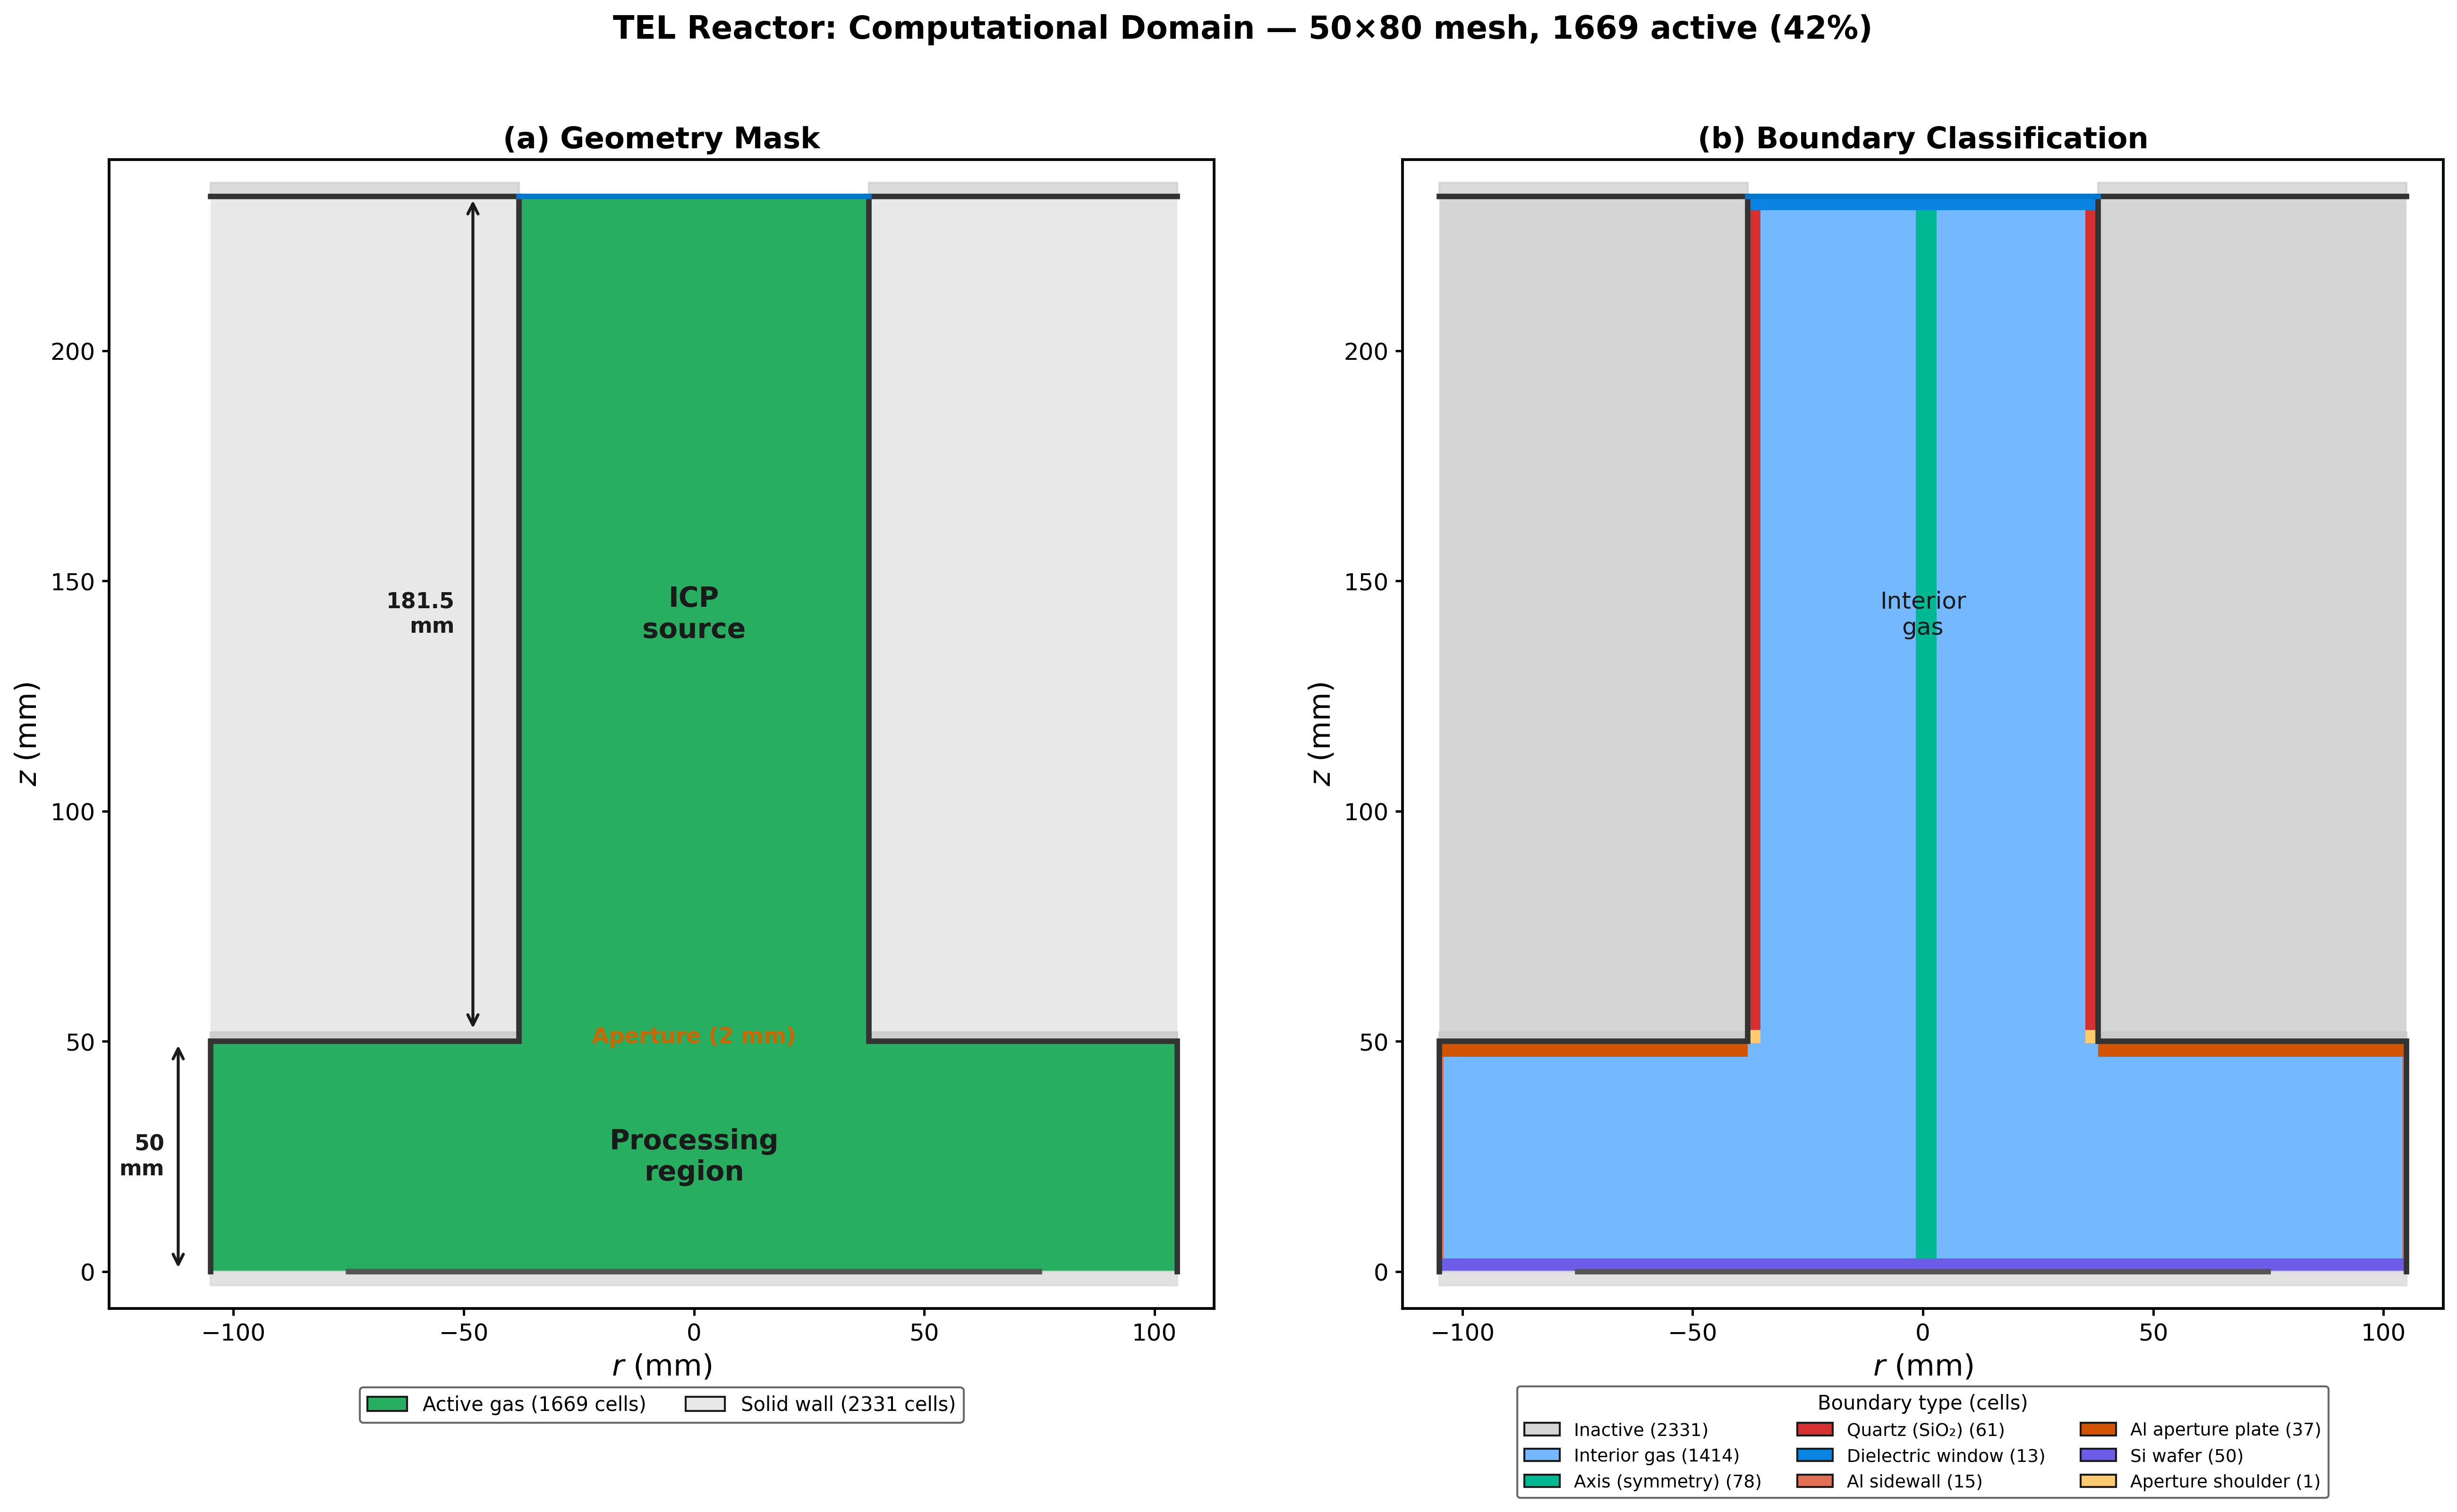
\includegraphics[width=0.9\linewidth]{geometry_mask.png}
\column{0.45\textwidth}
\small
\textbf{Last meeting:} validated 2D TEL fluid solver
\begin{itemize}\setlength\itemsep{0pt}
    \item Axisymmetric CCP reactor, T-shaped geometry
    \item SF\textsubscript{6}/Ar feed gas, 54 reactions
    \item Structured mesh, steady-state solutions
    \item Mesh convergence within \hlnum{1.86\%} ($n_F$), \hlnum{4.89\%} ($n_e$)
\end{itemize}

\vspace{0.5em}
\muted{Since our last meeting, three new directions explored\ldots}
\end{columns}
\end{frame}

% ----------------------------------------------------------
%  SLIDE 3 --- Three Directions Pursued
% ----------------------------------------------------------
\begin{frame}{Since Our Last Meeting: Three Directions}
\begin{columns}[T]
\column{0.32\textwidth}
\centering
\textbf{1. PINN Surrogate}\\[0.5em]
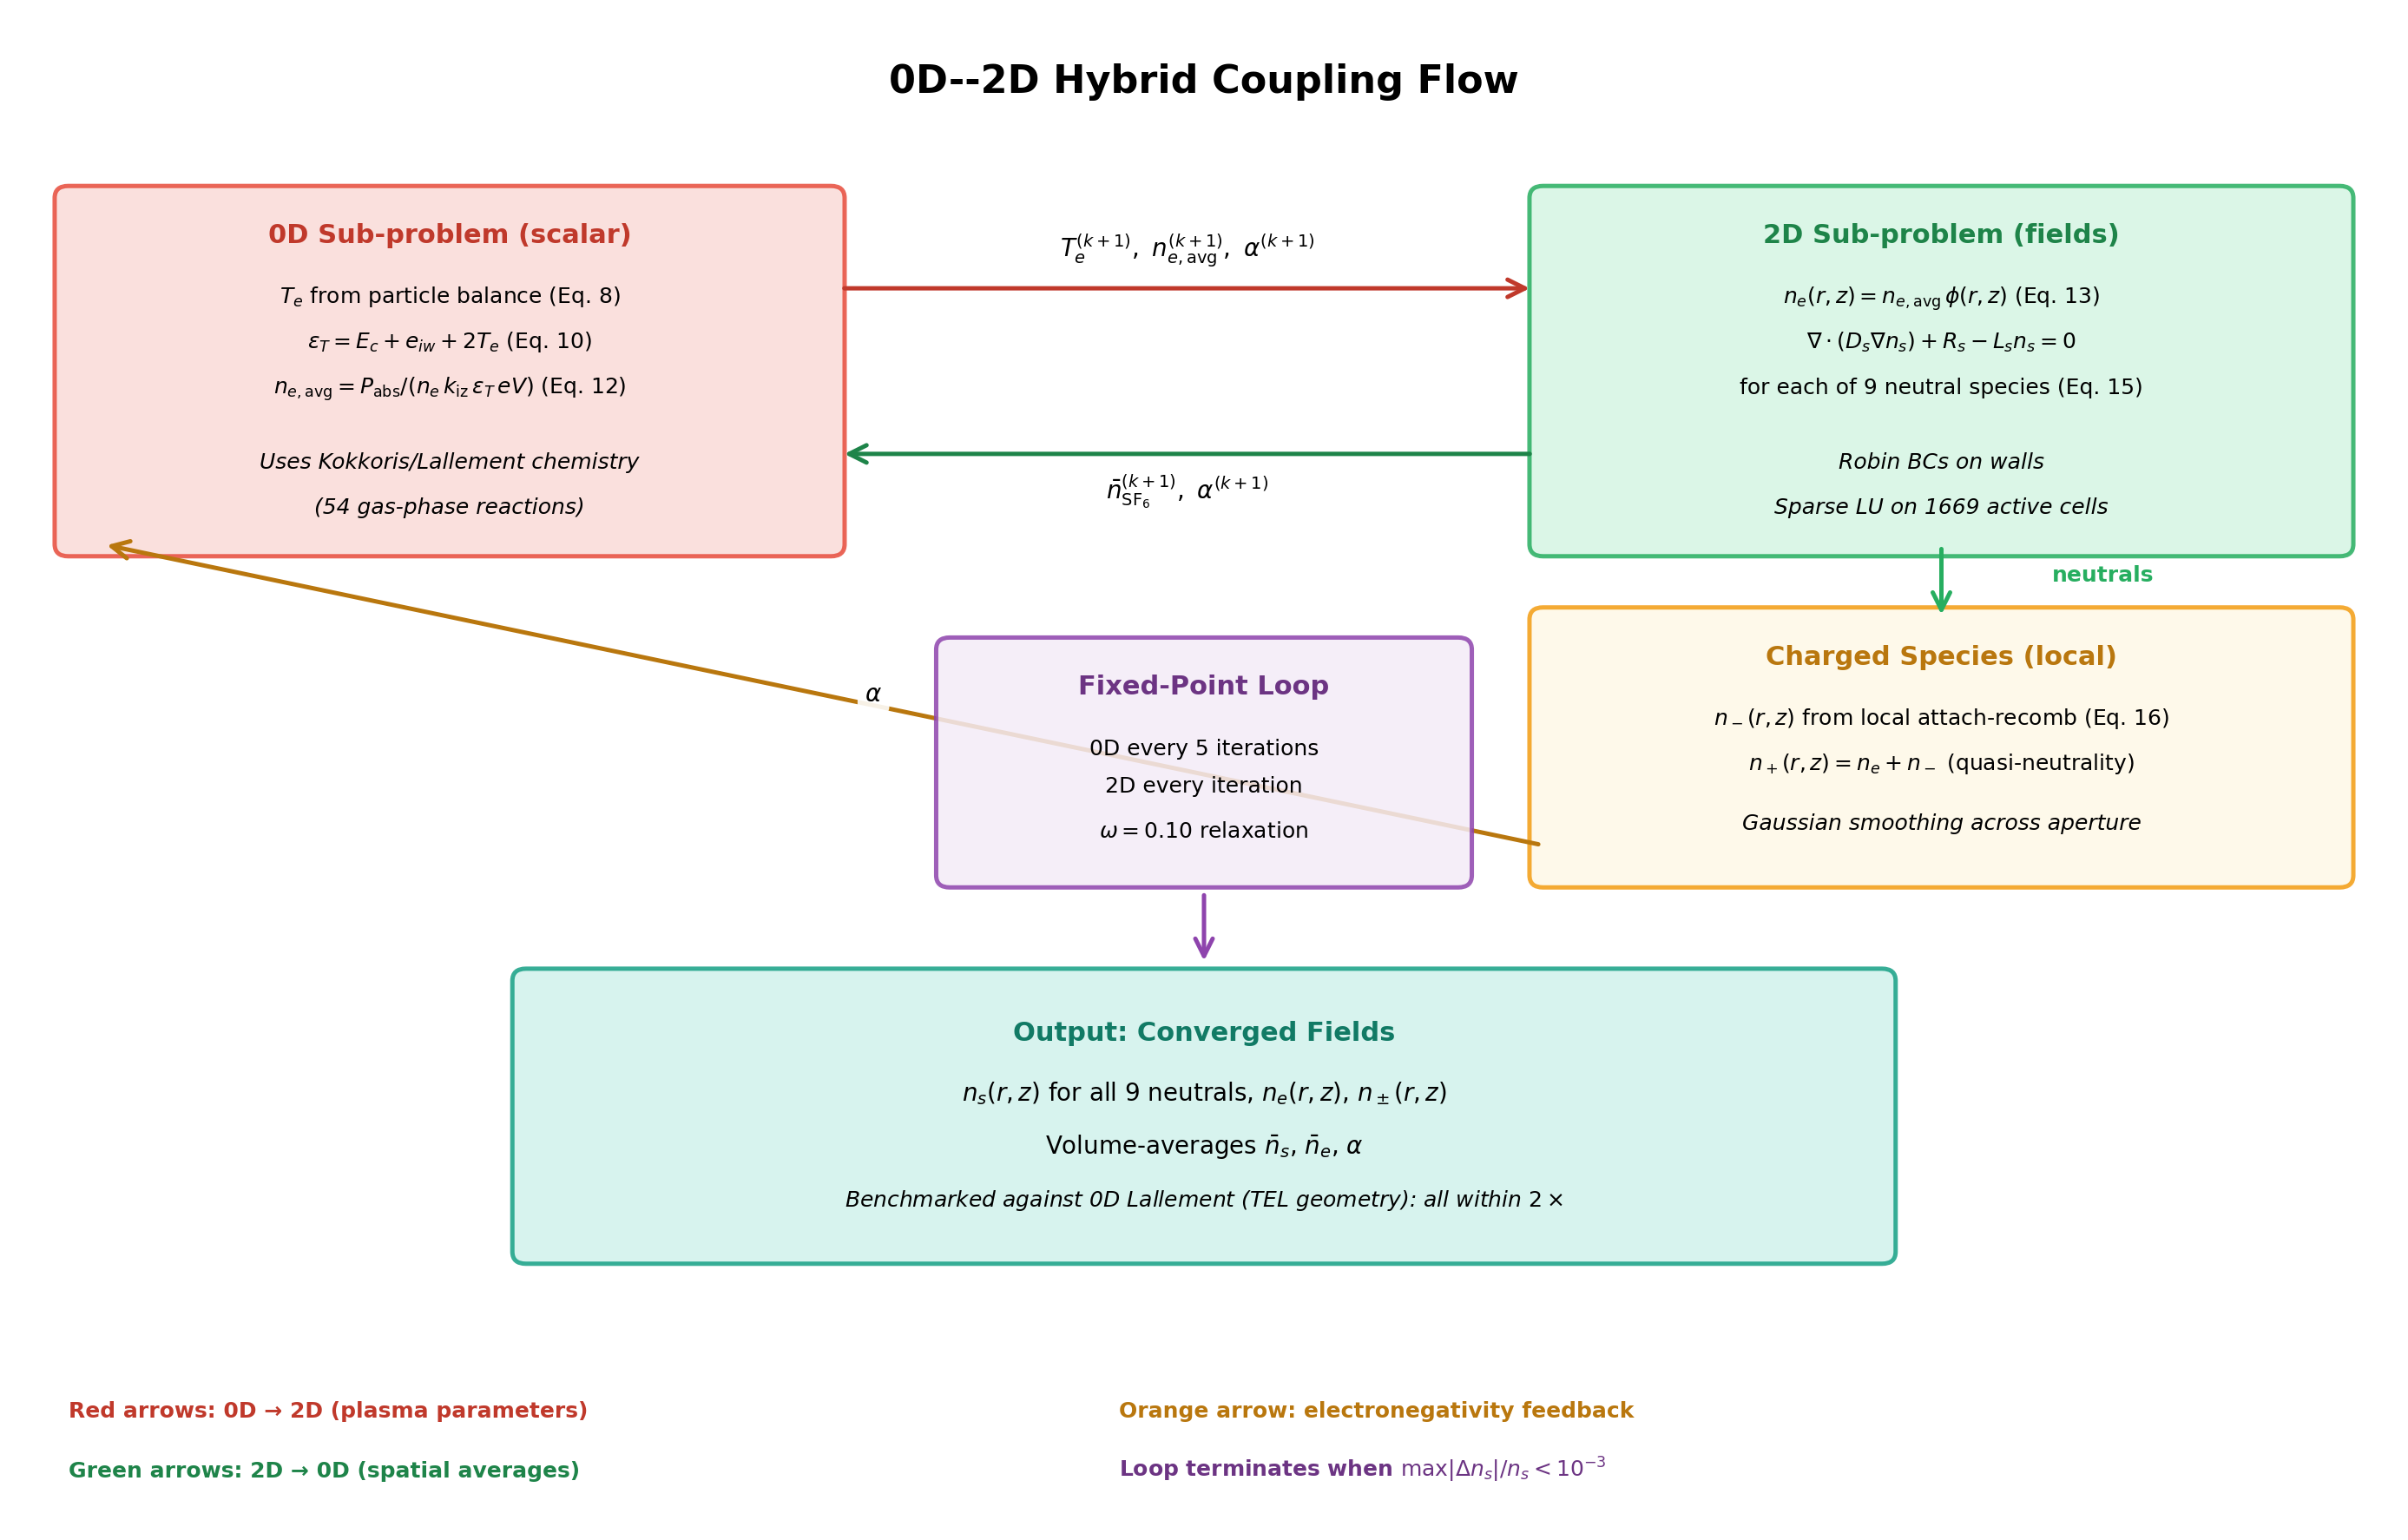
\includegraphics[width=0.75\linewidth]{coupling_flowchart.png}\\[0.2em]
\small PDE-constrained neural network\\
\bad{Failed} --- diverged

\column{0.32\textwidth}
\centering
\textbf{2. Supervised Surrogate}\\[0.5em]
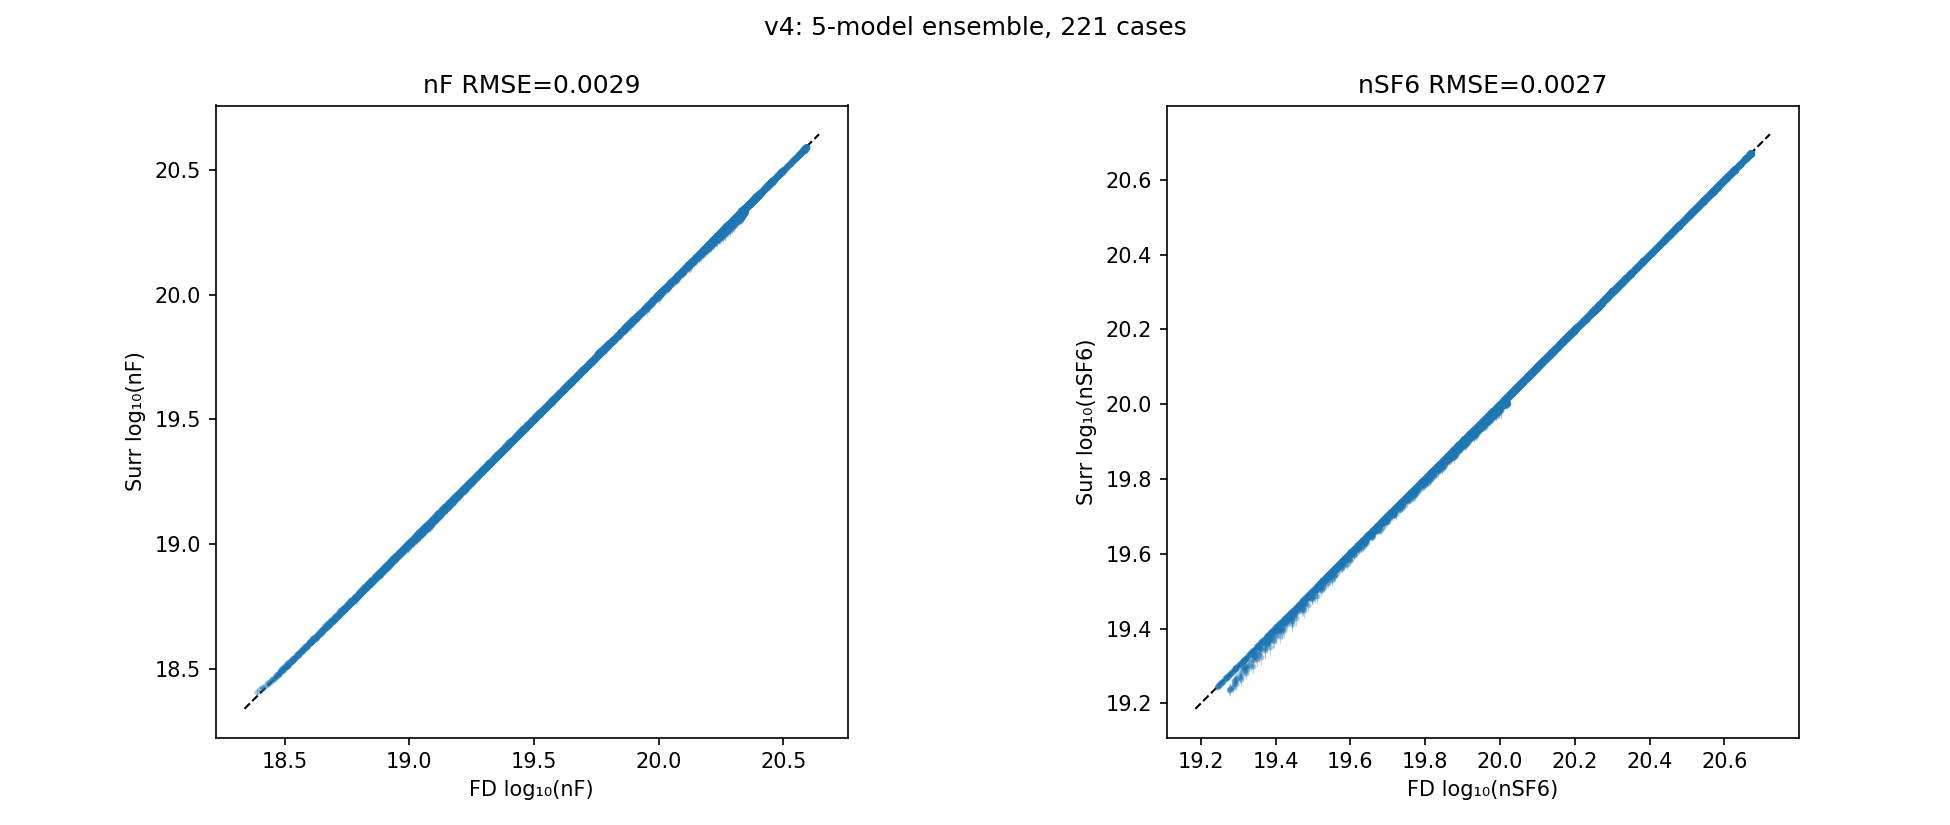
\includegraphics[width=0.75\linewidth]{surrogate_v4_pred_vs_true.png}\\[0.2em]
\small Fourier features + MLP\\
\good{Succeeded} --- RMSE 0.0015

\column{0.32\textwidth}
\centering
\textbf{3. LXCat Integration}\\[0.5em]
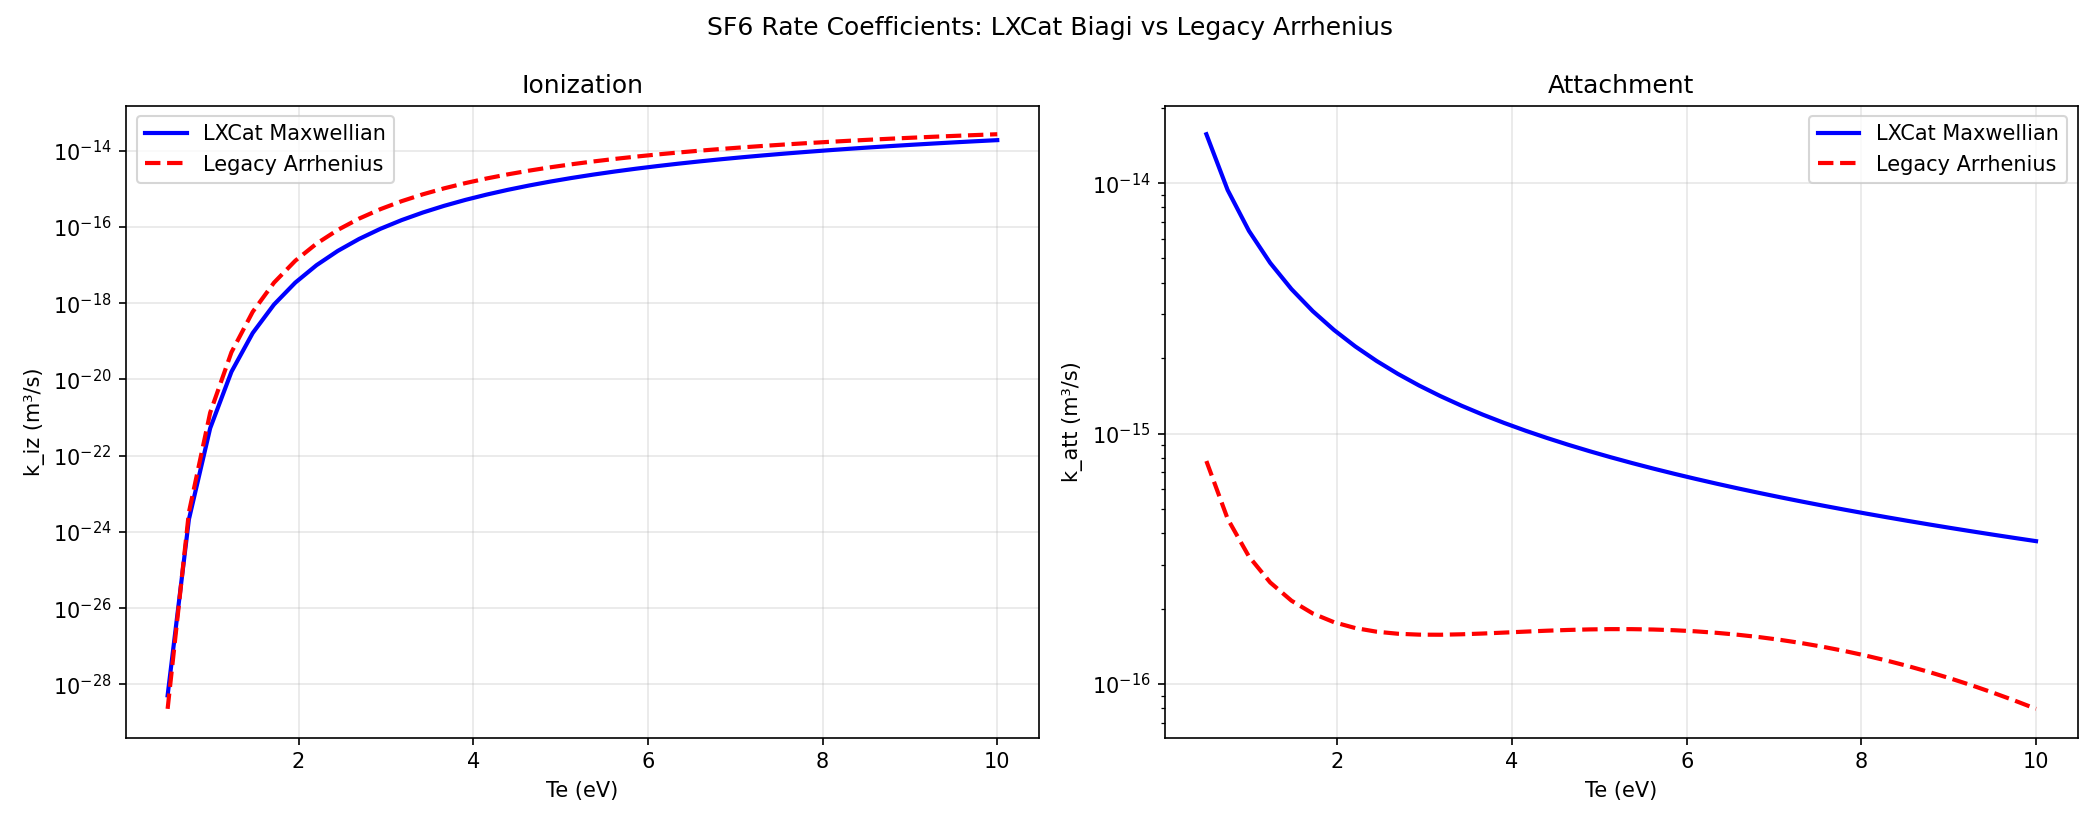
\includegraphics[width=0.75\linewidth]{lxcat_rate_comparison.png}\\[0.2em]
\small Biagi cross sections\\
Surprising conclusion
\end{columns}
\end{frame}

% ----------------------------------------------------------
%  SLIDE 4 --- PINN Attempt
% ----------------------------------------------------------
\begin{frame}{Direction 1: Physics-Informed Neural Network}
\begin{columns}[T]
\column{0.42\textwidth}
\centering
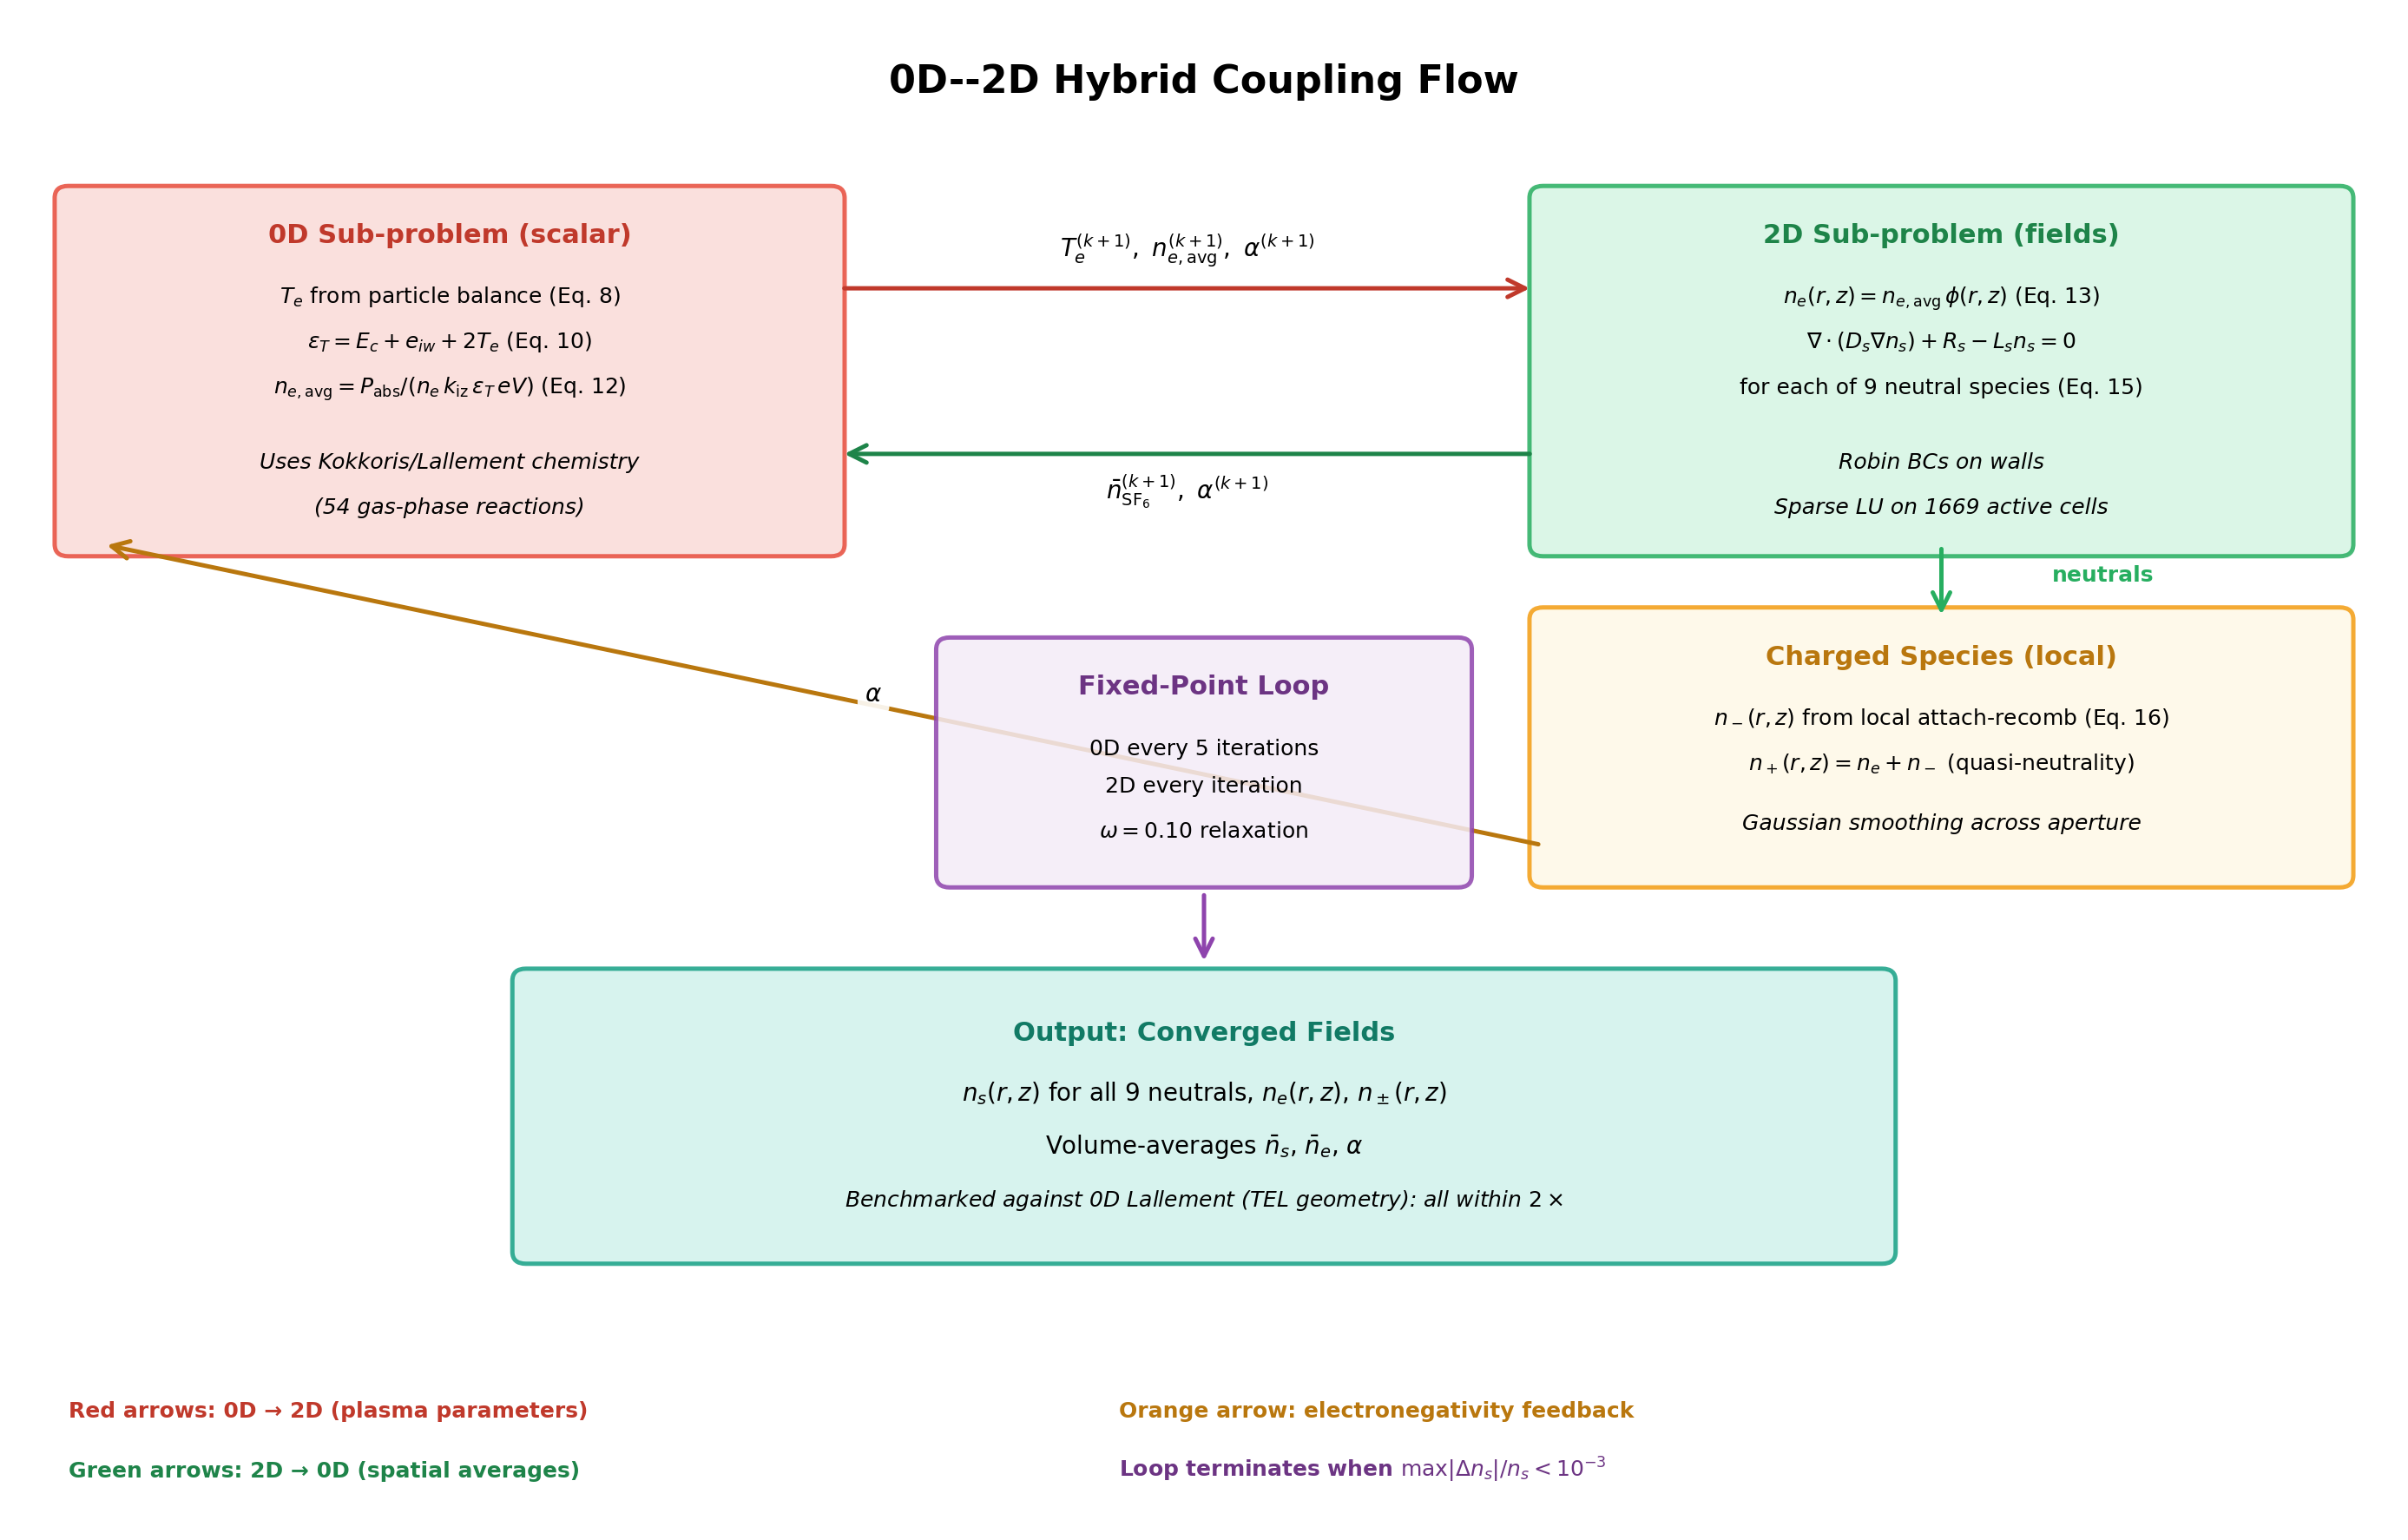
\includegraphics[width=0.8\linewidth]{coupling_flowchart.png}
\column{0.55\textwidth}
\small
\textbf{PDE-constrained PINN} --- \bad{diverges}
\begin{enumerate}\setlength\itemsep{0pt}
    \item Stiff 54-species chemistry defeats gradient descent
    \item Multi-scale densities cause loss imbalance
    \item Adaptive loss weighting cannot rescue convergence
\end{enumerate}

\vspace{0.3em}
\textbf{Data-only PINN:} converges, but \hlnum{23\,000$\times$} slower than plain MLP.

\vspace{0.3em}
$\Rightarrow$ \textbf{Pivot:} abandon PDE constraints, go fully supervised.
\end{columns}
\end{frame}

% ----------------------------------------------------------
%  SLIDE 5 --- Pivot to Supervised Surrogates
% ----------------------------------------------------------
\begin{frame}{Direction 2: Supervised Surrogate Architecture}
\begin{columns}[T]
\column{0.55\textwidth}
\small
\textbf{Architecture: Fourier Features + MLP}
\begin{itemize}\setlength\itemsep{0pt}
    \item Random Fourier features encode $(r, z)$
    \item Shared trunk + per-species output heads
    \item Inputs: power, pressure, composition, $(r,z)$
    \item Outputs: $\log_{10} n_F$, $\log_{10} n_{\text{SF}_6}$
\end{itemize}

\vspace{0.3em}
\textbf{Training recipe}
\begin{itemize}\setlength\itemsep{0pt}
    \item Bias init to physical mean density
    \item Cosine-annealing LR schedule
    \item 2000 epochs, batch size 4096
\end{itemize}
\column{0.42\textwidth}
\centering
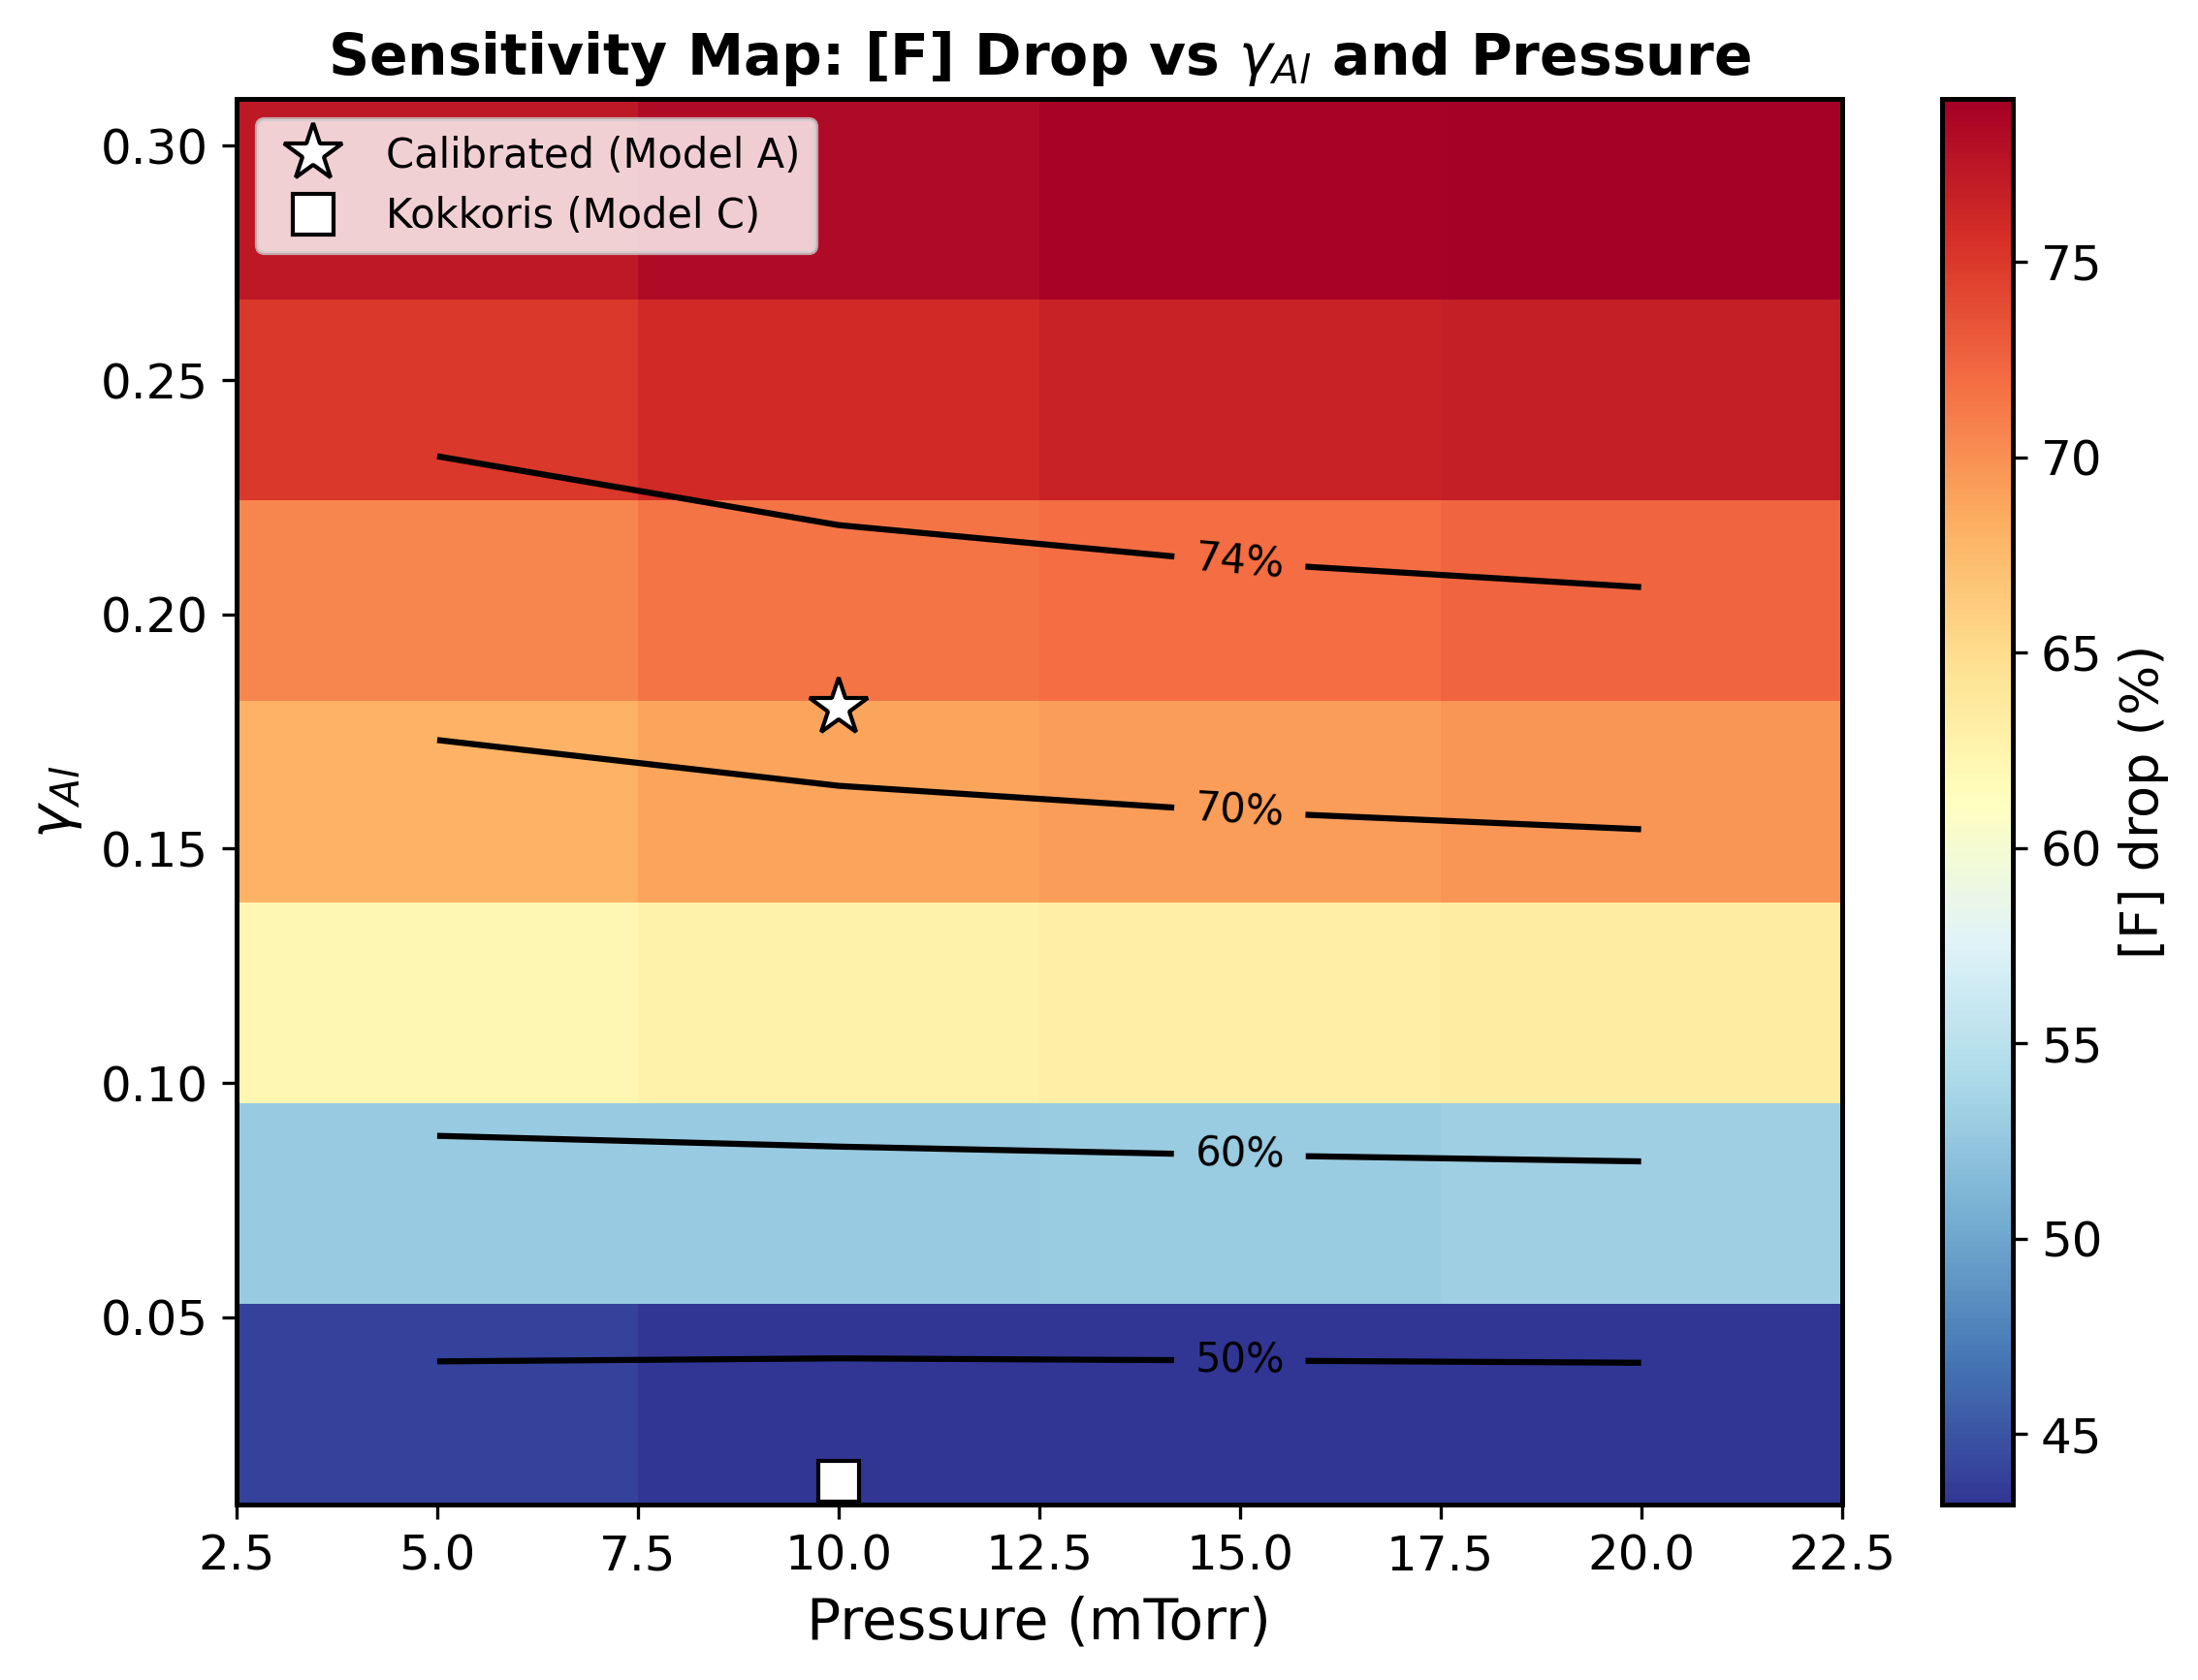
\includegraphics[width=0.85\linewidth]{sensitivity_map.png}\\
\small Input sensitivity map
\end{columns}
\end{frame}

% ----------------------------------------------------------
%  SLIDE 6 --- Surrogate Progression v1-v4
% ----------------------------------------------------------
\begin{frame}{Surrogate Progression: Four Generations}
\begin{columns}[T]
\column{0.48\textwidth}
\centering
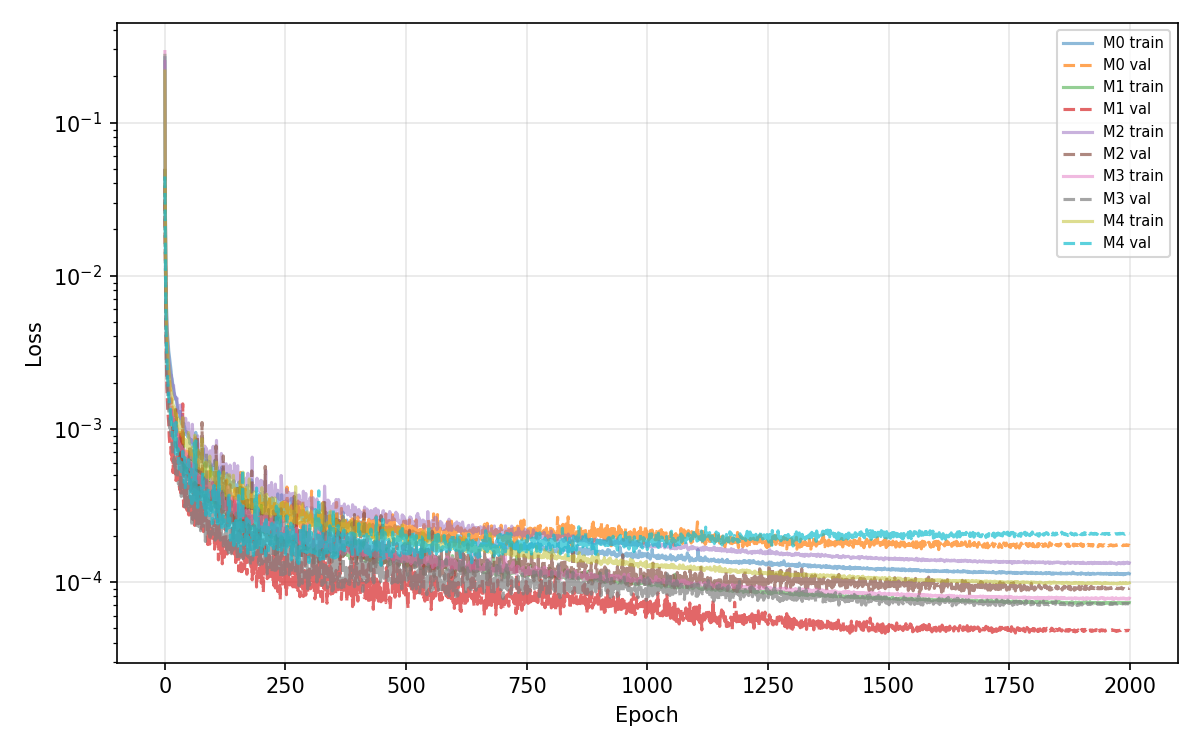
\includegraphics[width=0.9\linewidth]{surrogate_v4_loss_curves.png}\\
\small v4 training \& validation loss
\column{0.48\textwidth}
\centering
\begin{table}
\small
\begin{tabular}{@{}lcc@{}}
\toprule
\textbf{Version} & \textbf{RMSE} & \textbf{Key change} \\
\midrule
v1 & 0.133 & Naive MLP \\
v2 & 0.111 & Better normalisation \\
v3 & 0.023 & Fourier features \\
\textbf{v4} & \good{\textbf{0.003}} & Bias init + schedule \\
\bottomrule
\end{tabular}
\end{table}

\vspace{0.5em}
\hlnum{44$\times$} error reduction from v1 to v4.

\vspace{0.3em}
Each generation addressed a specific failure mode identified through residual analysis.
\end{columns}
\end{frame}

% ----------------------------------------------------------
%  SLIDE 7 --- Surrogate v4 Accuracy
% ----------------------------------------------------------
\begin{frame}{Surrogate v4: Prediction Accuracy}
\begin{columns}[T]
\column{0.48\textwidth}
\centering
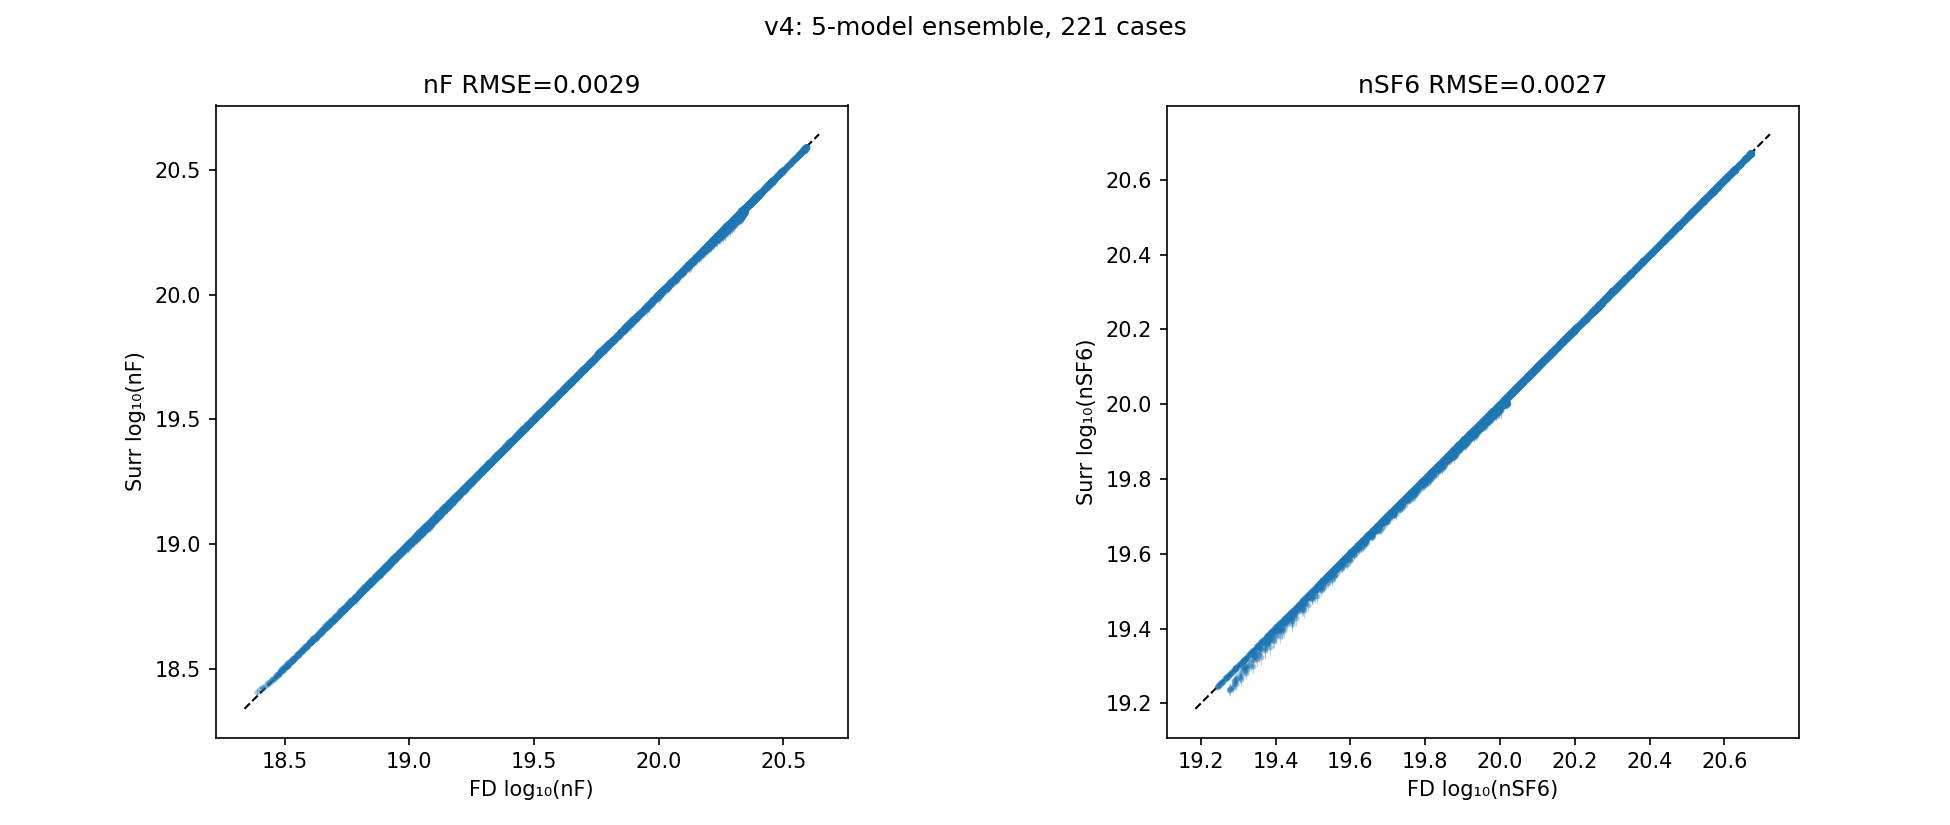
\includegraphics[width=0.9\linewidth]{surrogate_v4_pred_vs_true.png}\\
\small Predicted vs.\ true (all species)
\column{0.48\textwidth}
\centering
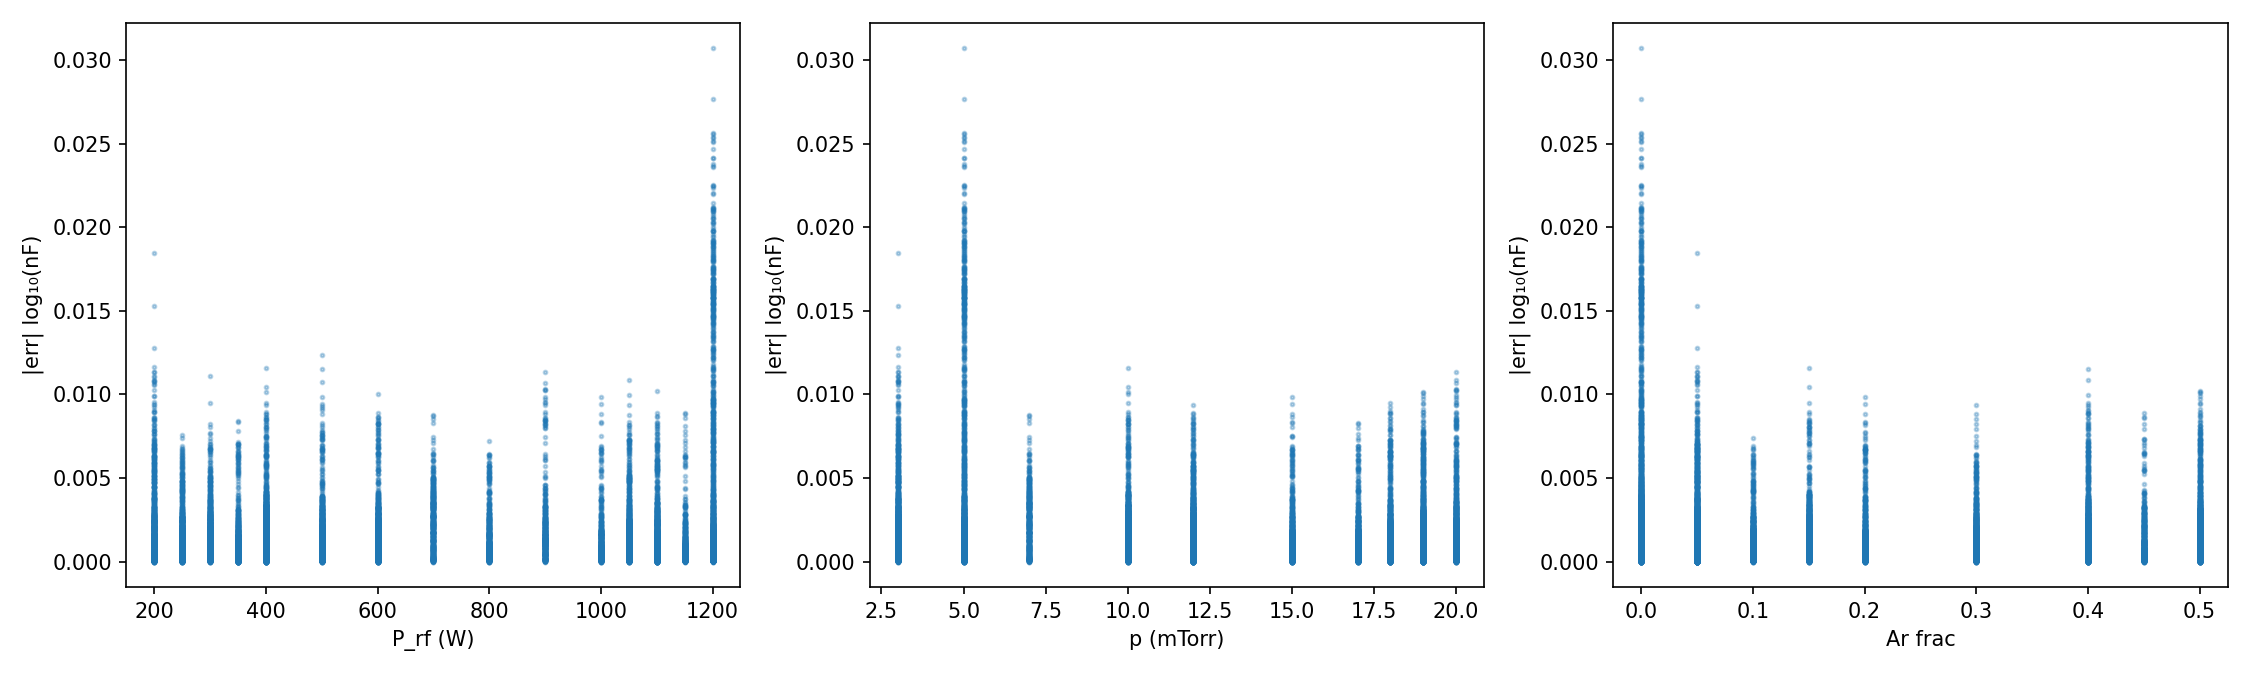
\includegraphics[width=0.9\linewidth]{surrogate_v4_diagnostics_nF.png}\\
\small $n_F$ residual diagnostics
\end{columns}

\vspace{0.3em}
\centering
\small Tight clustering along diagonal; residuals are symmetric, homoscedastic, and spatially uniform.
\end{frame}

% ----------------------------------------------------------
%  SLIDE 8 --- LXCat Integration
% ----------------------------------------------------------
\begin{frame}[shrink=5]{Direction 3: LXCat Cross-Section Integration}
\begin{columns}[T]
\column{0.48\textwidth}
\centering
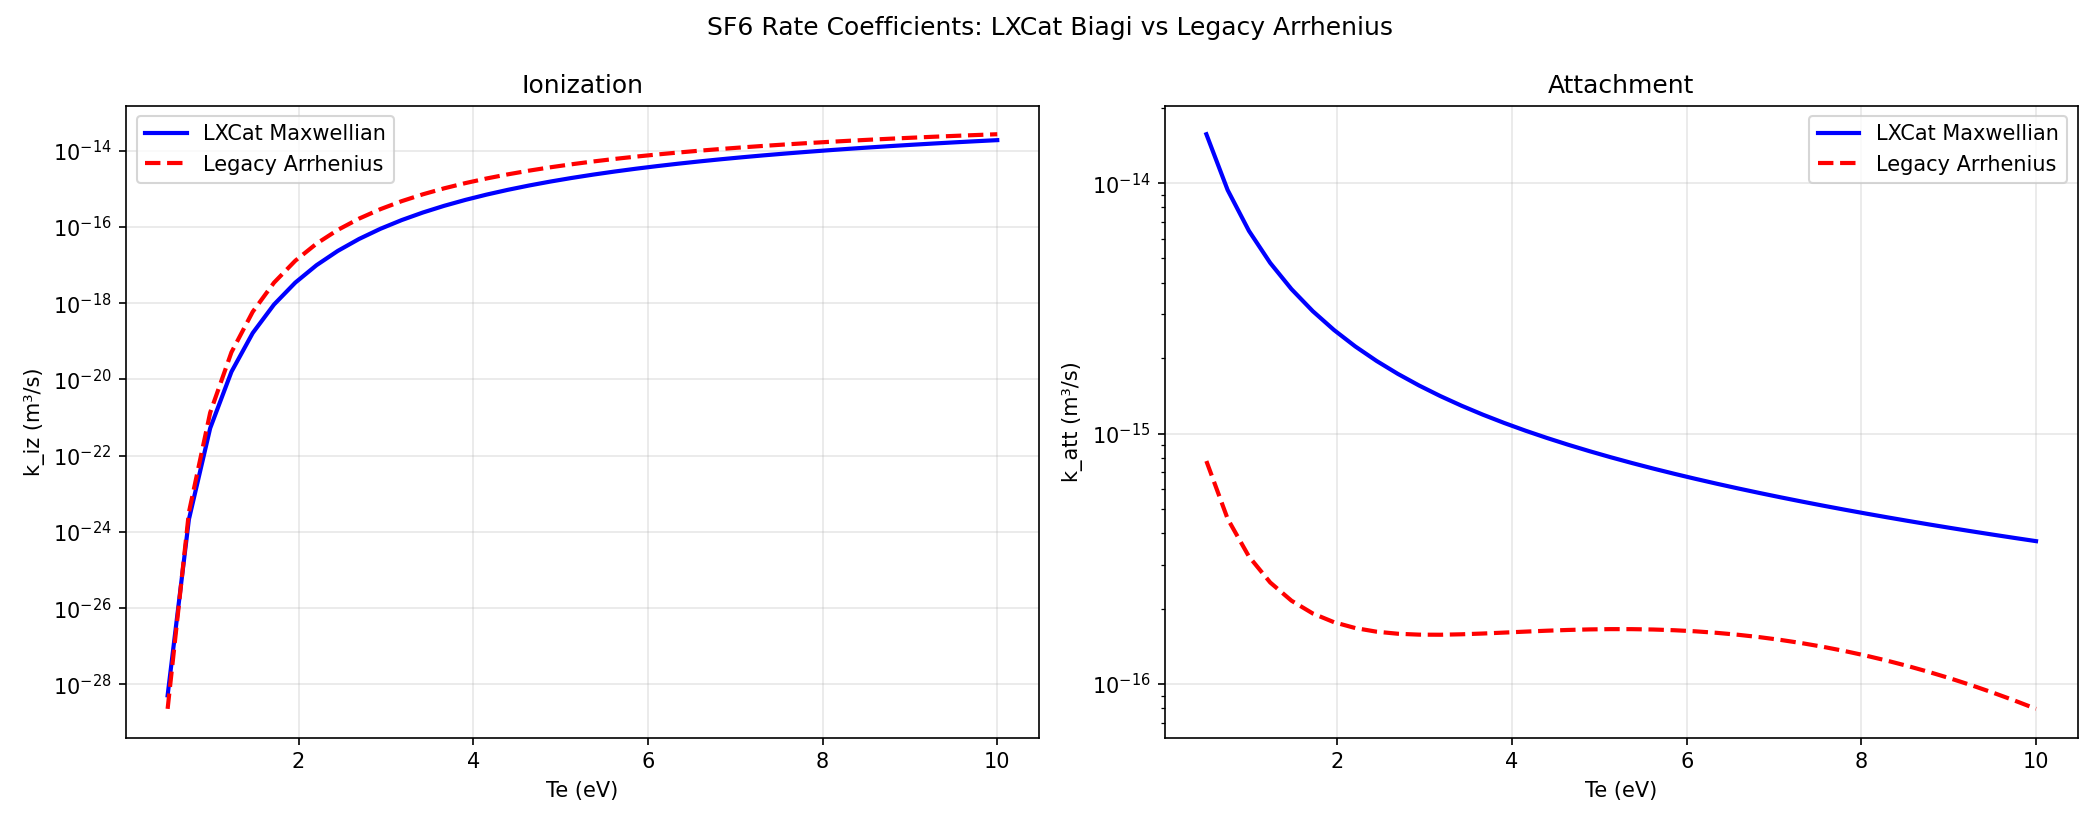
\includegraphics[width=0.9\linewidth]{lxcat_rate_comparison.png}\\
\small Rate coefficient comparison
\column{0.48\textwidth}
\textbf{What changed}
\begin{itemize}
    \item Replaced legacy cross sections with Biagi (LXCat) database
    \item Solver option: \texttt{rate\_mode='lxcat'}
    \item Boltzmann-solver--computed rate coefficients
\end{itemize}

\vspace{0.5em}
\textbf{Physics impact on solver outputs}
\begin{itemize}
    \item $T_e$: \bad{$+56\%$} increase
    \item $n_e$: \bad{$-69\%$} decrease
    \item F density: \good{unchanged}
\end{itemize}

\vspace{0.3em}
Electron kinetics shift dramatically; neutral chemistry is robust.
\end{columns}
\end{frame}

% ----------------------------------------------------------
%  SLIDE 9 --- LXCat Physics Impact
% ----------------------------------------------------------
\begin{frame}{LXCat: Wafer-Level Impact}
\centering
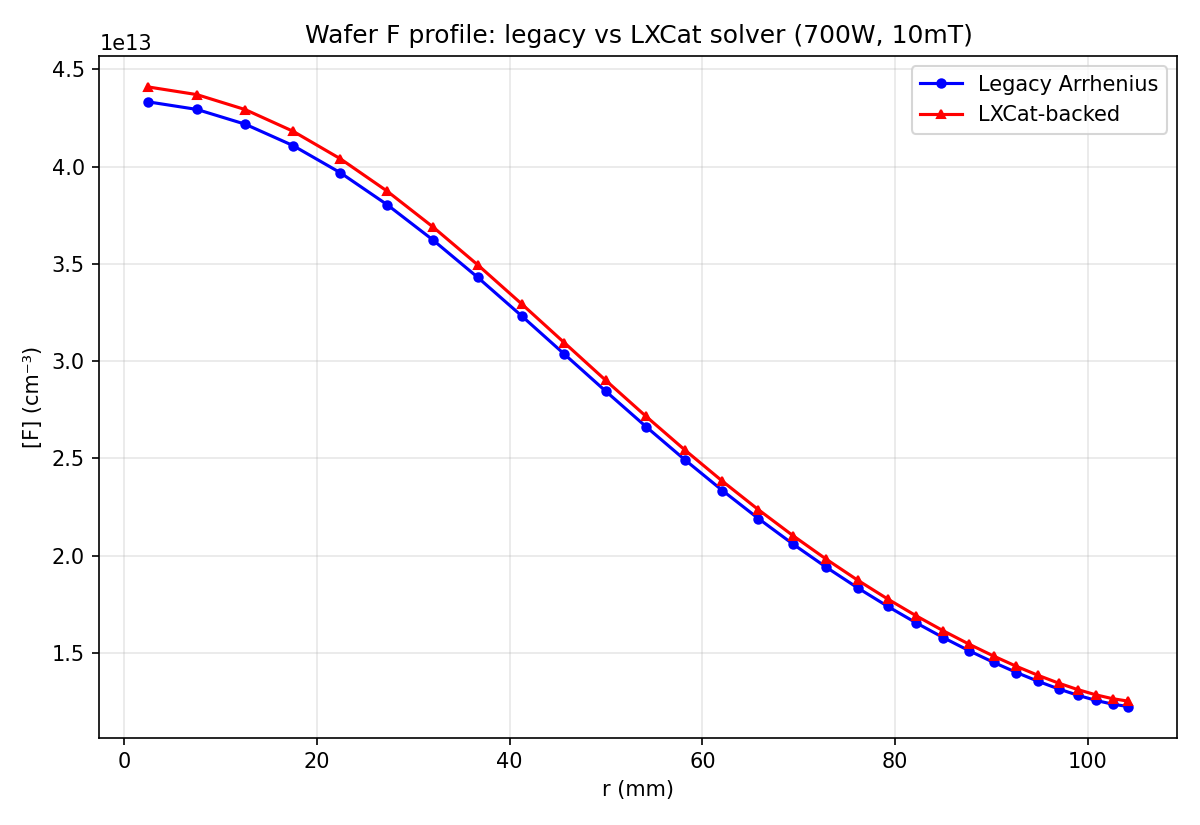
\includegraphics[width=0.6\linewidth]{lxcat_solver_wafer_profile.png}

\vspace{0.2em}
\small F density at wafer nearly identical between legacy and LXCat --- etch-relevant quantity is insensitive to electron kinetics.
\end{frame}

% ----------------------------------------------------------
%  SLIDE 10 --- The Surprise: Dataset Diagnosis
% ----------------------------------------------------------
\begin{frame}[shrink=3]{The Surprise: It Was Never the Data}
\begin{columns}[T]
\column{0.55\textwidth}
\small
\textbf{Hypothesis:} LXCat data is ``harder'' to learn.

\vspace{0.3em}
\textbf{Finding:} Datasets are \hlnum{statistically identical}.

\vspace{0.3em}
\textbf{Evidence:}
\begin{itemize}\setlength\itemsep{0pt}
    \item lxcat\_v3 RMSE: \bad{0.01124}
    \item Legacy v4 RMSE: \good{0.00292}
    \item Same architecture, same data volume
    \item Difference: \textbf{training recipe only}
\end{itemize}

\vspace{0.3em}
$\Rightarrow$ Gap was bias init + scheduling, not cross-section quality.

\column{0.42\textwidth}
\centering
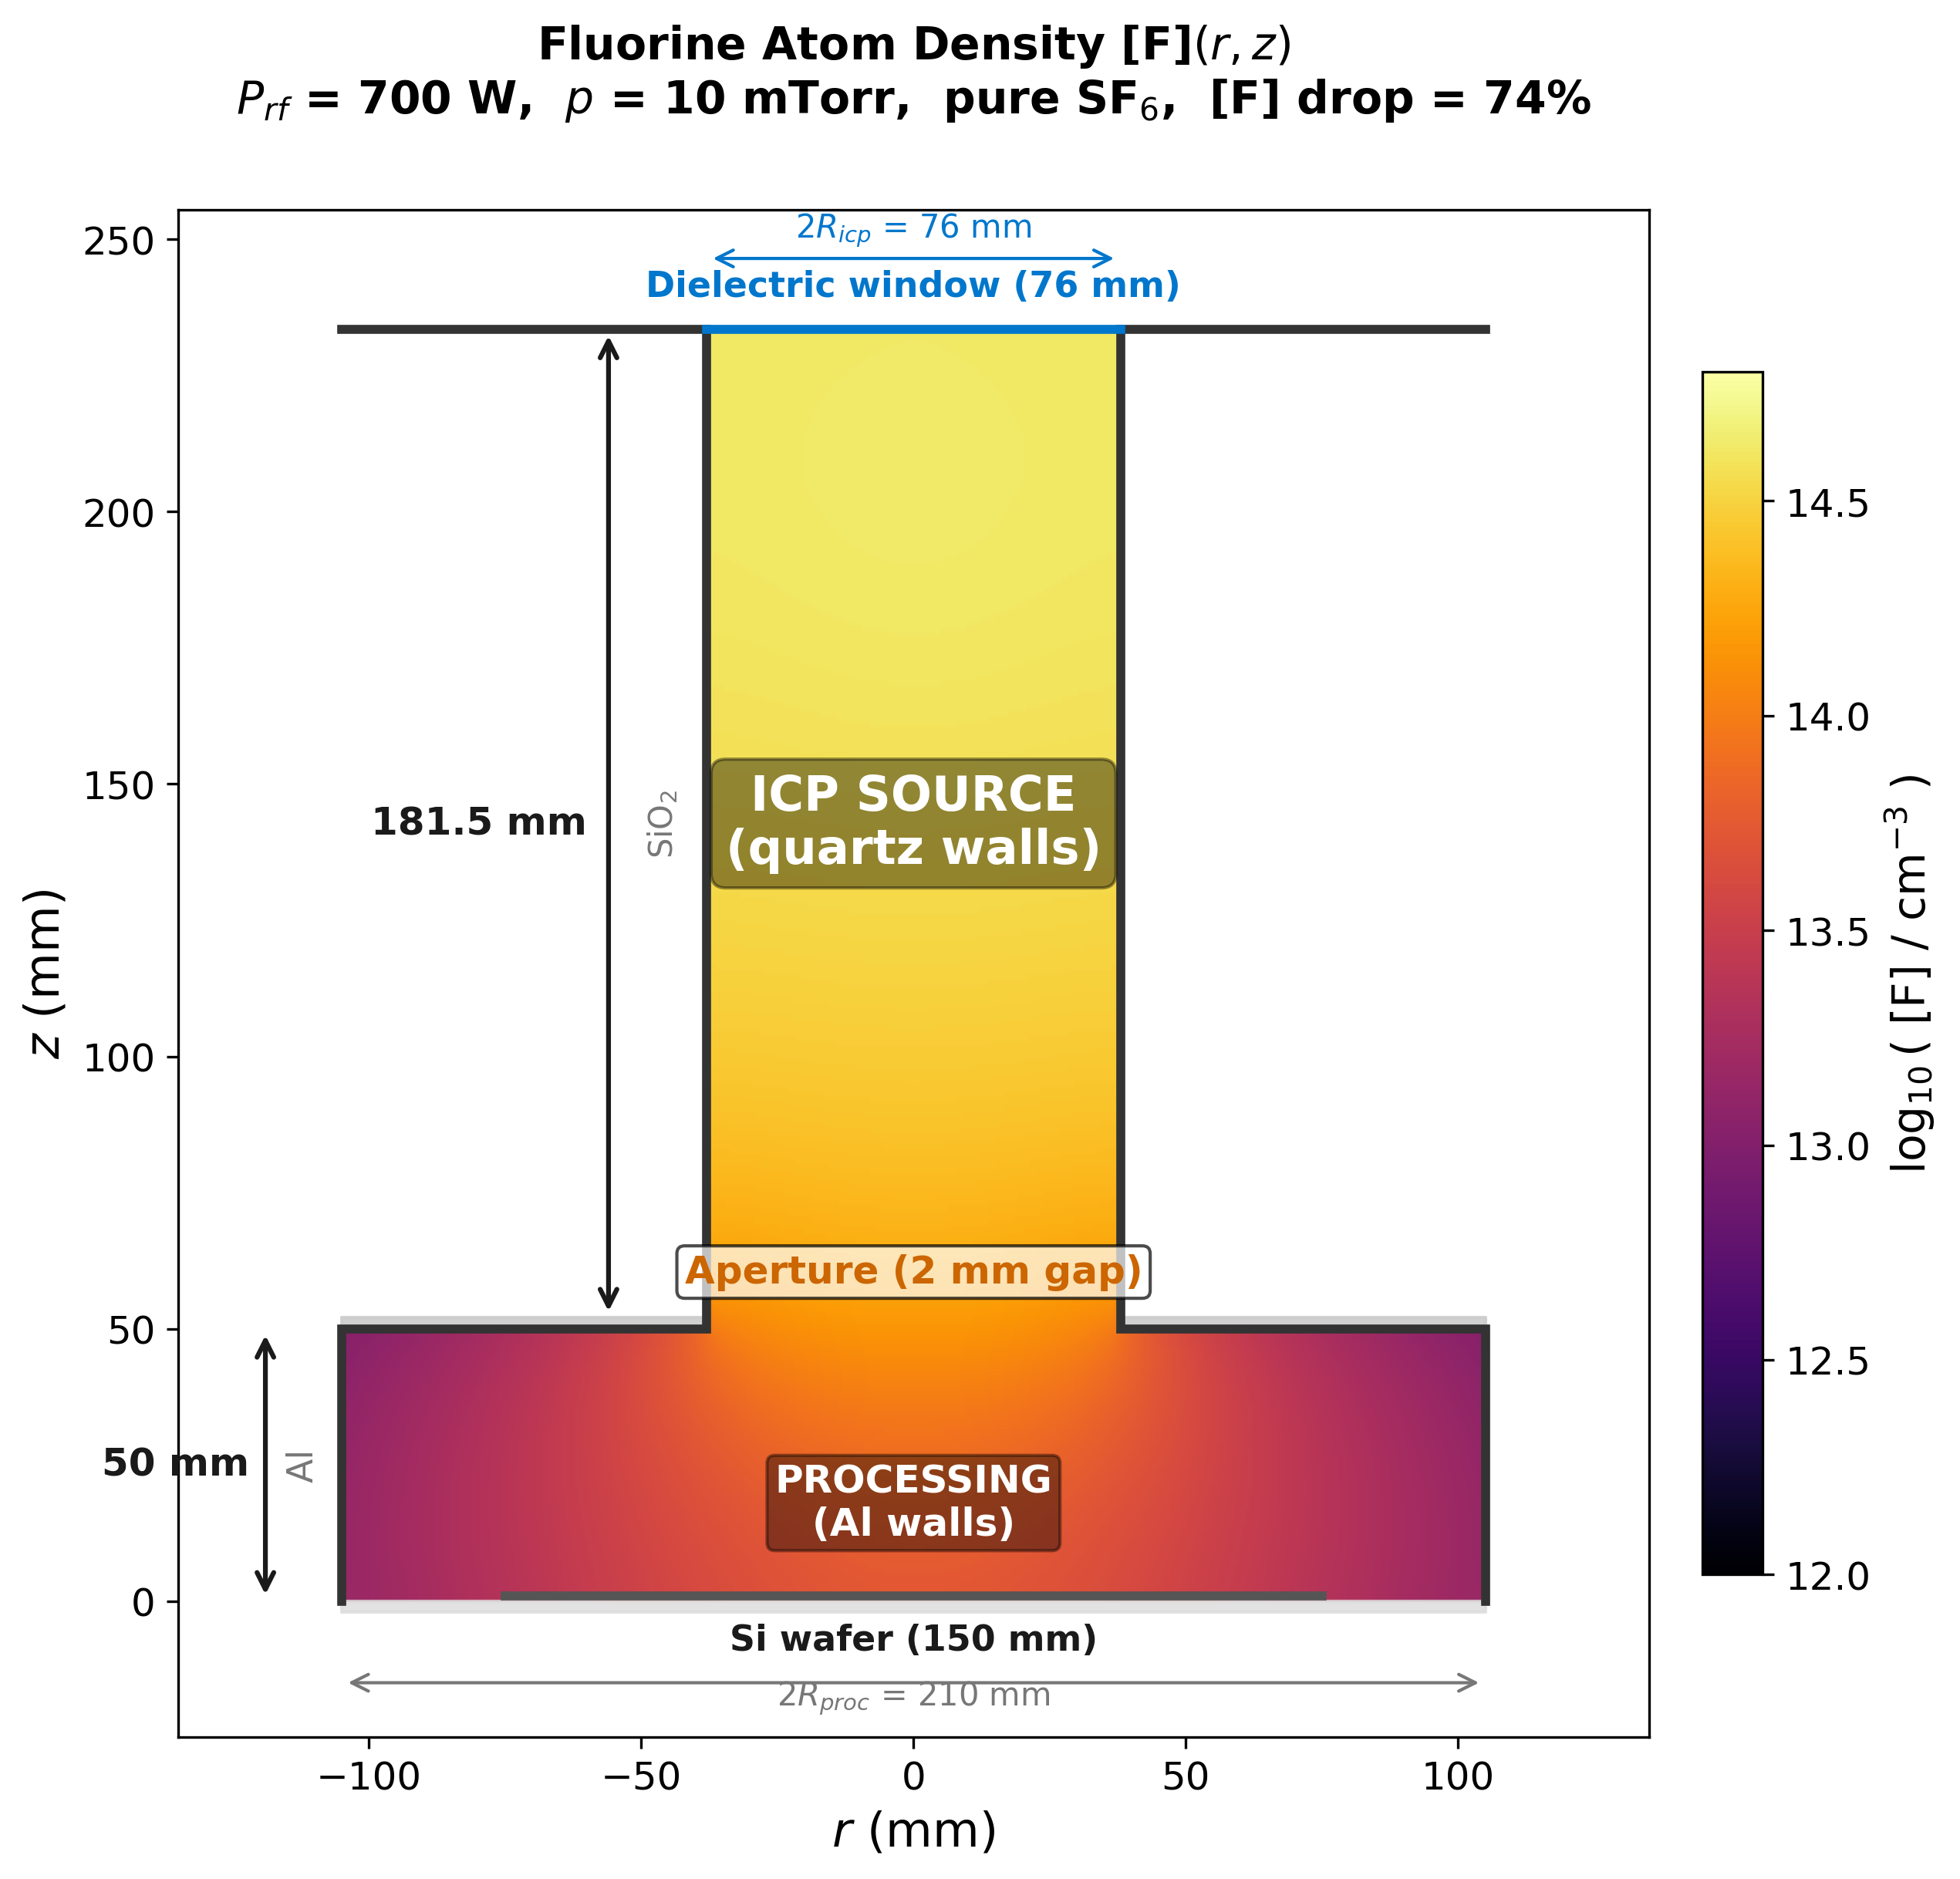
\includegraphics[width=0.85\linewidth]{cross_sections.png}\\
\small Cross-section sets overlap
\end{columns}
\end{frame}

% ----------------------------------------------------------
%  SLIDE 11 --- Architecture Sweep
% ----------------------------------------------------------
\begin{frame}{Architecture Sweep: 7 Experiments}
\centering
\begin{table}
\centering
\begin{tabular}{@{}llcc@{}}
\toprule
\textbf{ID} & \textbf{Architecture} & \textbf{RMSE} & \textbf{$\Delta$ vs.\ E0} \\
\midrule
E0 & Vanilla MLP (baseline)             & 0.01901 & --- \\
E1 & Wider hidden layers (512)          & 0.00377 & $-80\%$ \\
E2 & Deeper network (6 layers)          & 0.00390 & $-79\%$ \\
\rowcolor{good!15}
E3 & \textbf{Shared trunk + separate heads} & \good{\textbf{0.00210}} & \good{$-89\%$} \\
E4 & Residual connections               & 0.00244 & $-87\%$ \\
E5 & Dropout regularisation             & 0.00957 & $-50\%$ \\
E6 & Batch normalisation                & 0.00394 & $-79\%$ \\
\bottomrule
\end{tabular}
\end{table}

\vspace{0.5em}
\textbf{Winner:} \hlnum{E3 --- separate heads}. Shared trunk learns common physics; per-species heads capture distinct density scales.
\end{frame}

% ----------------------------------------------------------
%  SLIDE 12 --- Ablation Study
% ----------------------------------------------------------
\begin{frame}{Ablation: What Actually Drives Accuracy?}
\centering
\begin{table}
\centering
\begin{tabular}{@{}lccc@{}}
\toprule
\textbf{Configuration} & \textbf{RMSE} & \textbf{$\Delta$ vs.\ none} & \textbf{Verdict} \\
\midrule
None (no tricks)           & 0.01830 & ---          & Baseline \\
Bias init only             & 0.00314 & $-83\%$      & \good{Dominant} \\
Regularisation only        & 0.01888 & $+3\%$       & \bad{Useless} \\
More epochs only           & 0.01610 & $-12\%$      & Marginal \\
All three combined         & 0.00385 & $-79\%$      & Mostly bias init \\
\bottomrule
\end{tabular}
\end{table}

\vspace{0.8em}
\textbf{Bias initialisation alone} accounts for \hlnum{83\%} of the improvement.\\
Physics regularisation adds nothing; extra epochs give only 12\%.
\end{frame}

% ----------------------------------------------------------
%  SLIDE 13 --- Production Ensemble
% ----------------------------------------------------------
\begin{frame}[shrink=5]{Production Ensemble: Final Numbers}
\begin{columns}[T]
\column{0.48\textwidth}
\centering
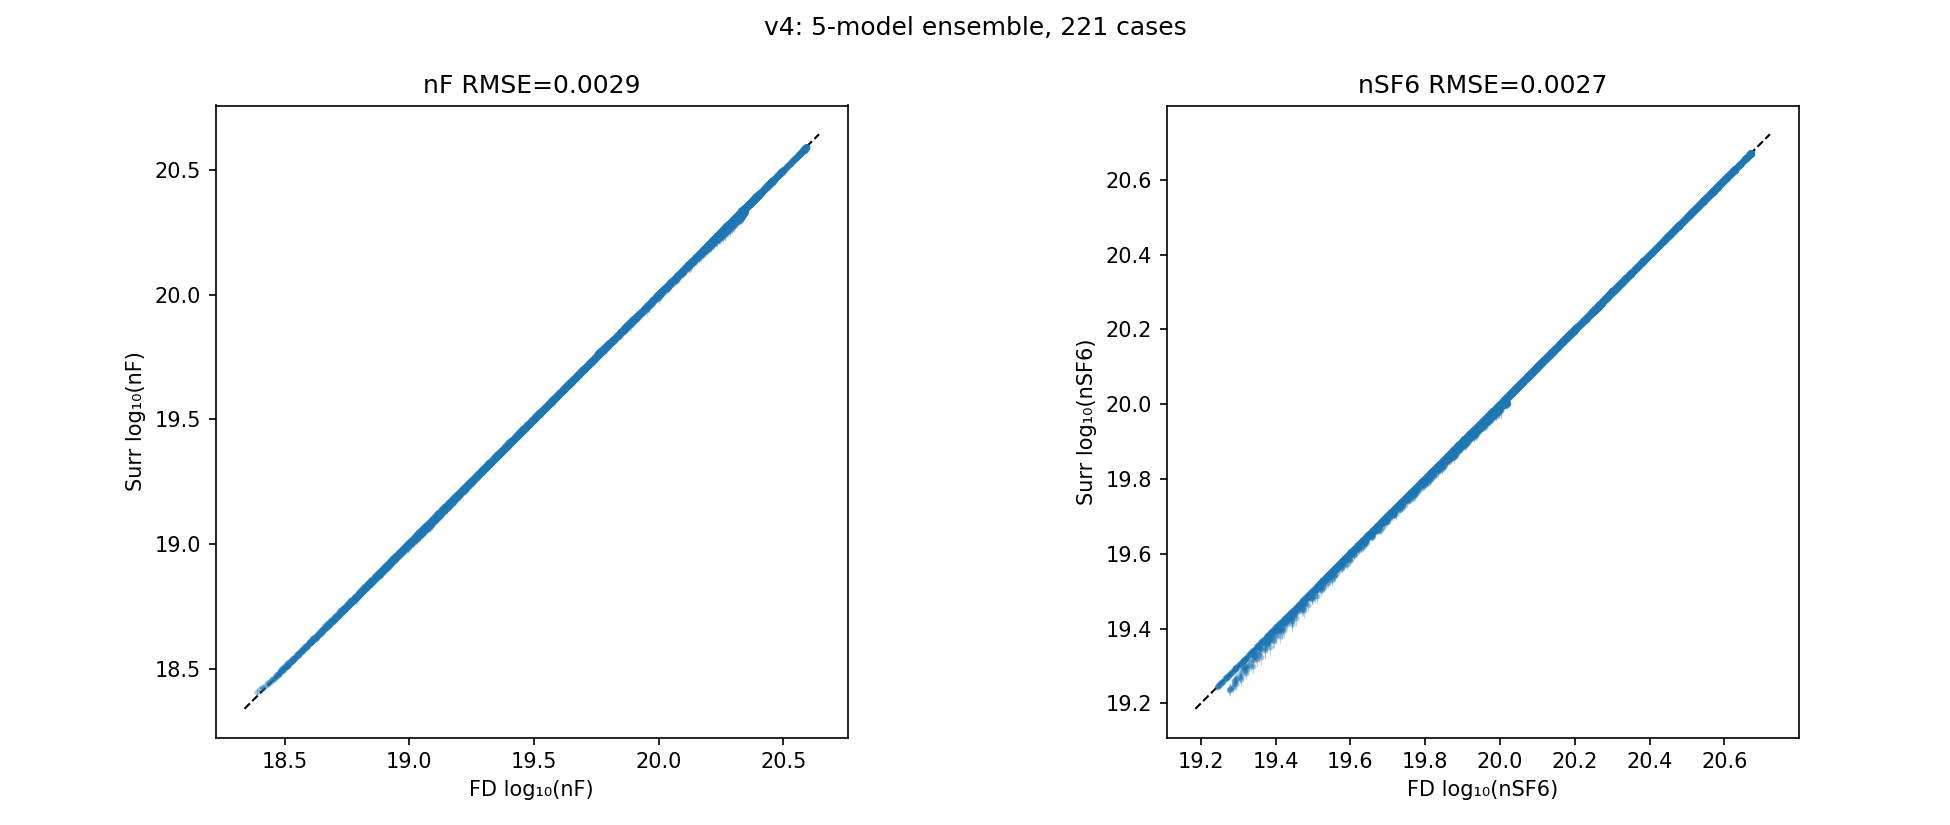
\includegraphics[width=0.85\linewidth]{surrogate_v4_pred_vs_true.png}\\
\small Predicted vs.\ true
\column{0.48\textwidth}
\small
\textbf{Ensemble RMSE}
\begin{itemize}\setlength\itemsep{0pt}
    \item $n_F$: \hlnum{0.00154}
    \item $n_{\text{SF}_6}$: \hlnum{0.00128}
\end{itemize}

\vspace{0.3em}
\textbf{vs.\ legacy v4}
\begin{itemize}\setlength\itemsep{0pt}
    \item $n_F$: 0.00292 $\to$ 0.00154
    \item $n_{\text{SF}_6}$: 0.00270 $\to$ 0.00128
\end{itemize}

\vspace{0.3em}
Beats legacy v4 by \hlnum{47\%} on $n_F$.

\vspace{0.3em}
\centering
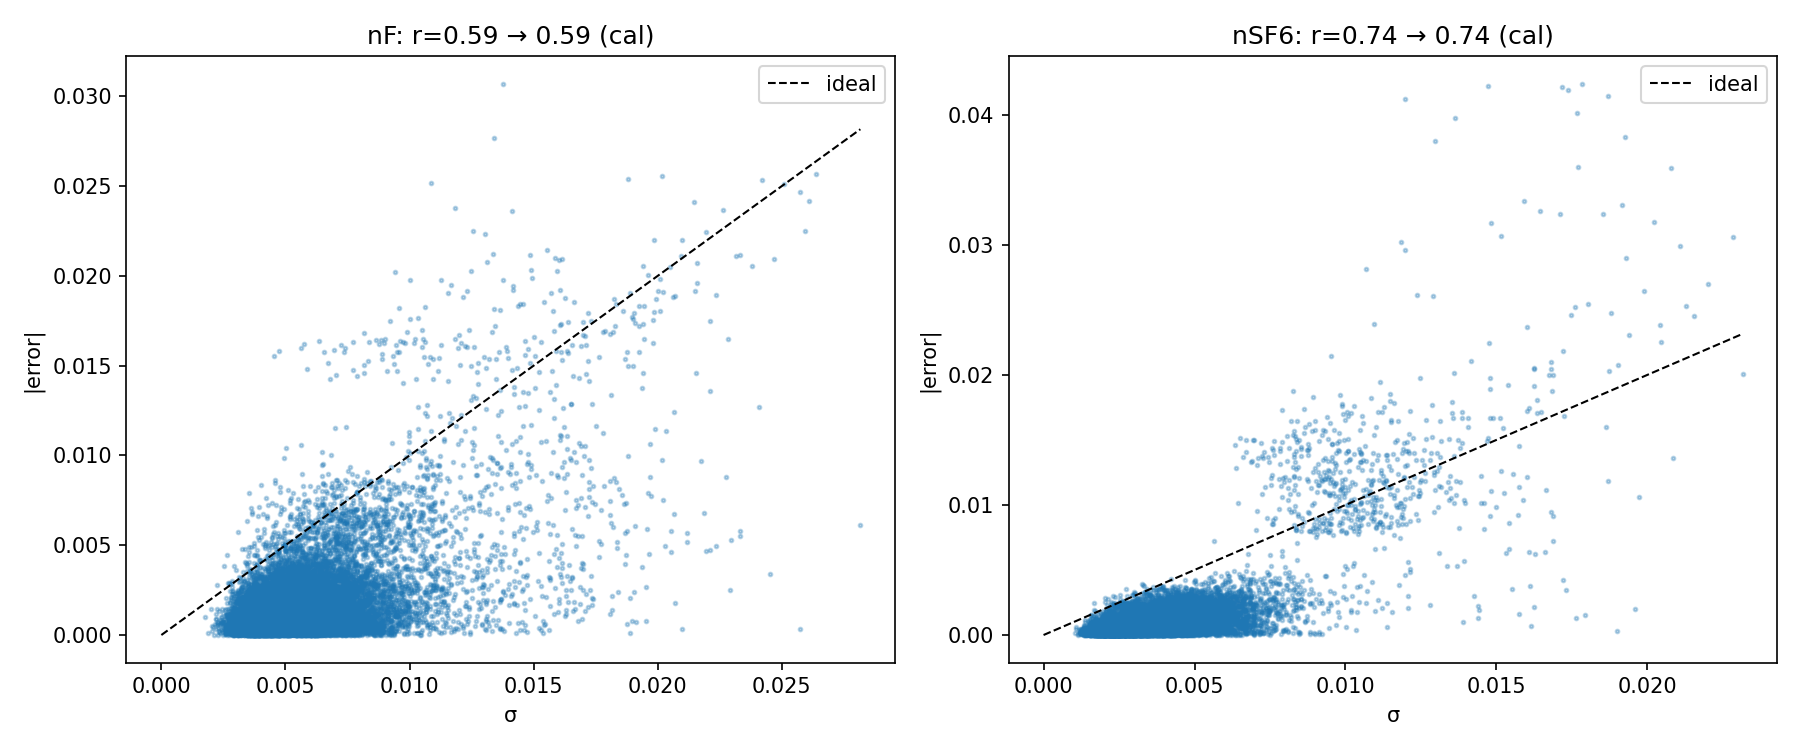
\includegraphics[width=0.75\linewidth]{surrogate_v4_uncertainty.png}\\
\small Ensemble uncertainty
\end{columns}
\end{frame}

% ----------------------------------------------------------
%  SLIDE 14 --- Solver Validation Against Literature
% ----------------------------------------------------------
\begin{frame}{Solver Validation Against Literature}
\begin{columns}[T]
\column{0.48\textwidth}
\centering
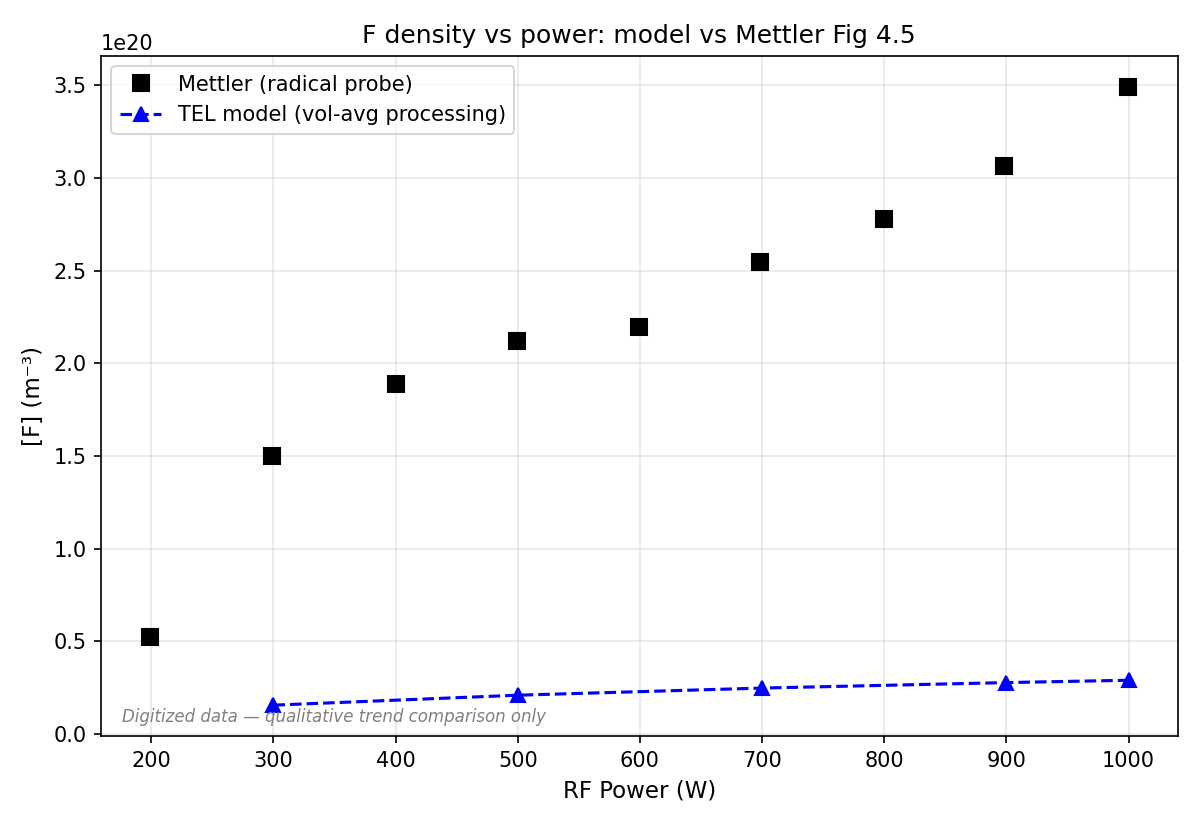
\includegraphics[width=0.9\linewidth]{lit_F_vs_power.png}\\
\small F density vs.\ power --- \bad{36\% error}
\column{0.48\textwidth}
\centering
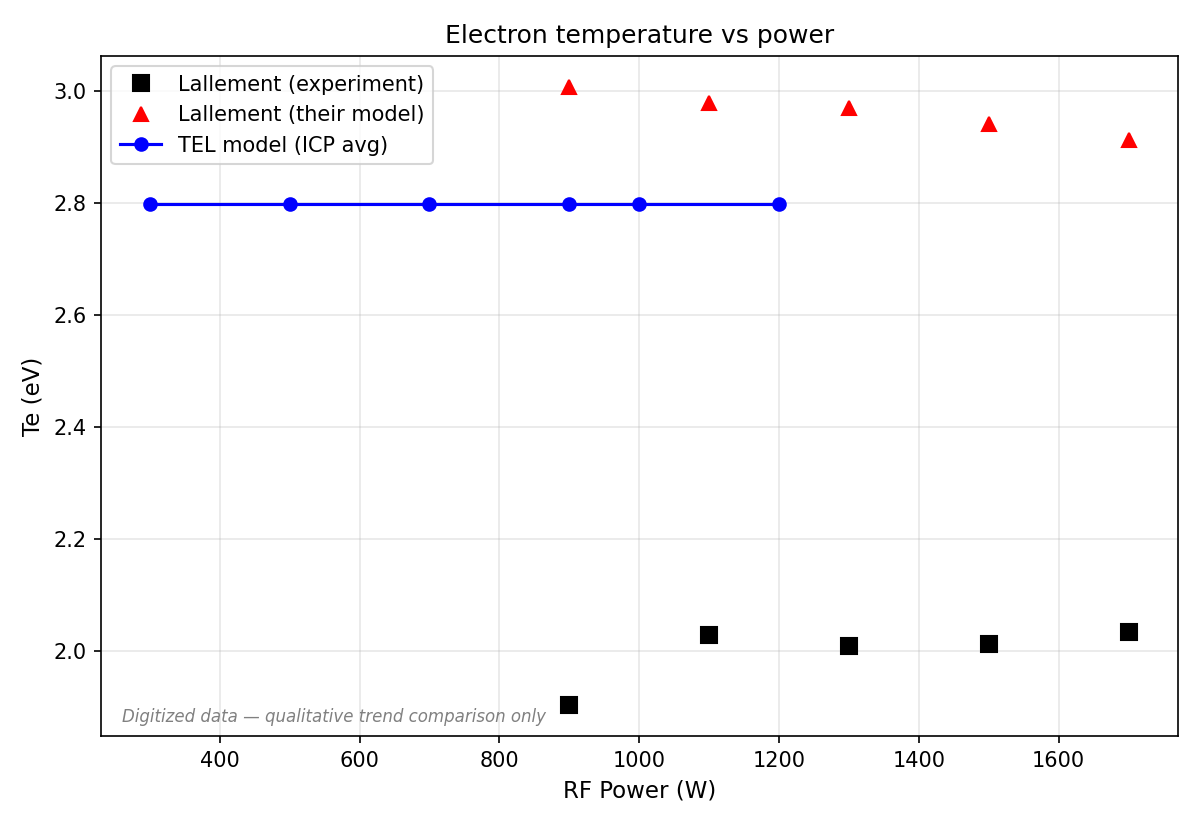
\includegraphics[width=0.9\linewidth]{lit_Te_vs_power.png}\\
\small $T_e$ vs.\ power --- Legacy: \bad{5\%}; LXCat: \bad{58\%}
\end{columns}

\vspace{0.3em}
\centering
\small Solver reproduces qualitative trends. Quantitative offsets set the accuracy ceiling for any surrogate trained on this data.
\end{frame}

% ----------------------------------------------------------
%  SLIDE 15 --- Spatial Error Distribution
% ----------------------------------------------------------
\begin{frame}{Spatial Error: Uniform Across Reactor Regions}
\begin{columns}[T]
\column{0.48\textwidth}
\centering
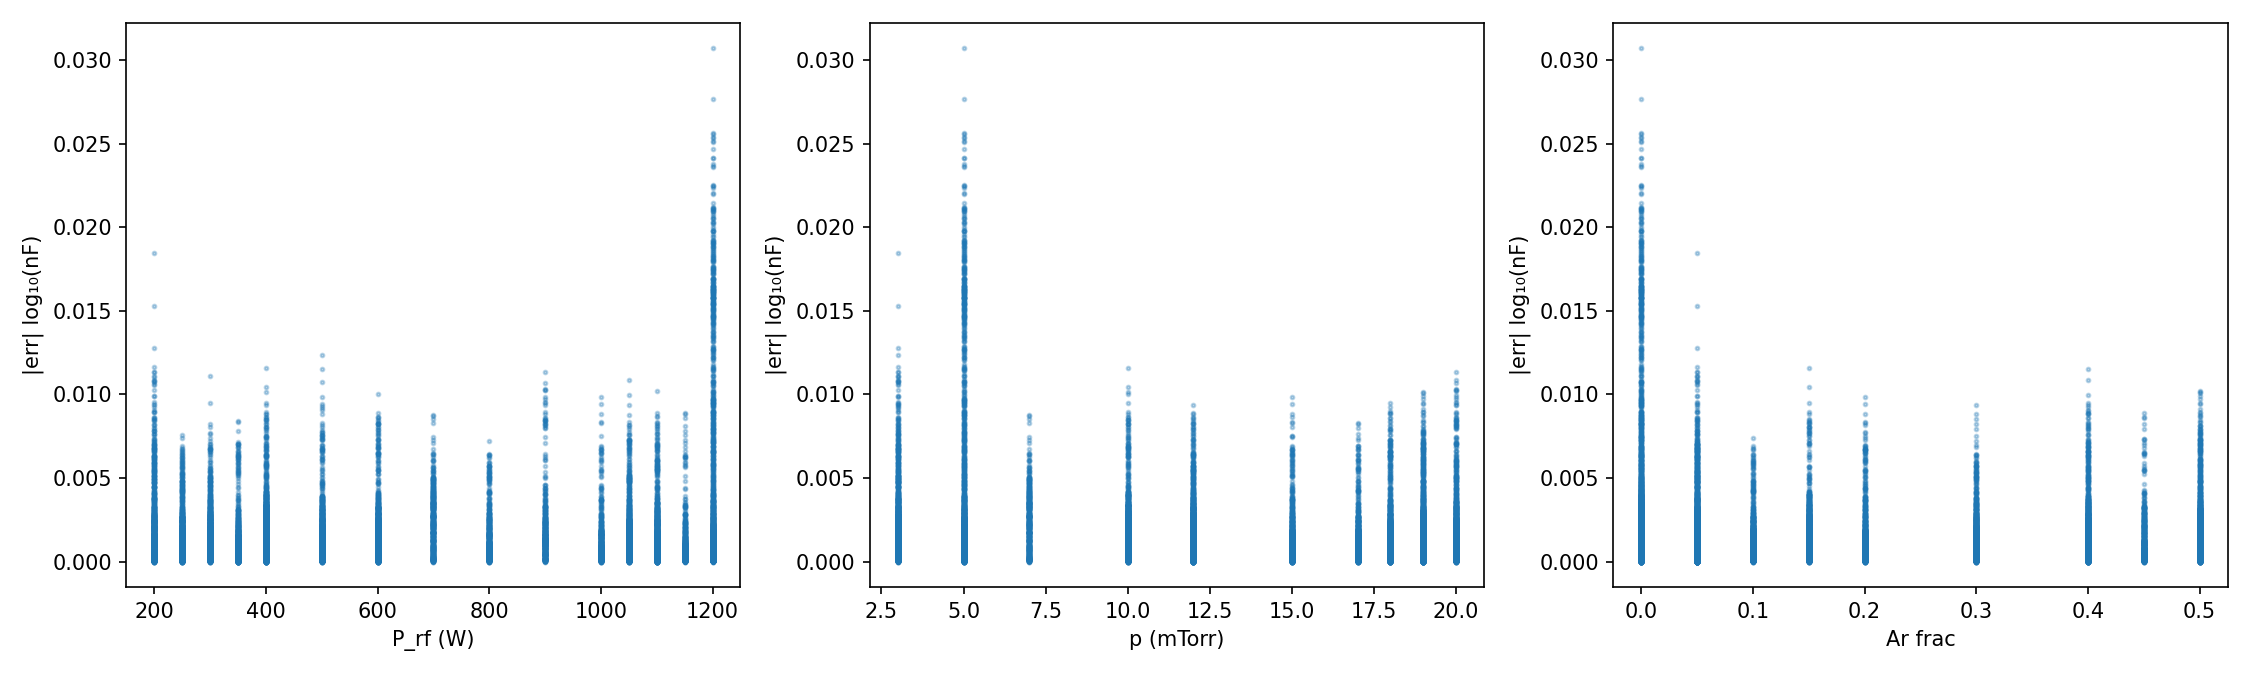
\includegraphics[width=0.85\linewidth]{surrogate_v4_diagnostics_nF.png}\\
\small $n_F$ residuals --- no spatial bias
\column{0.48\textwidth}
\centering
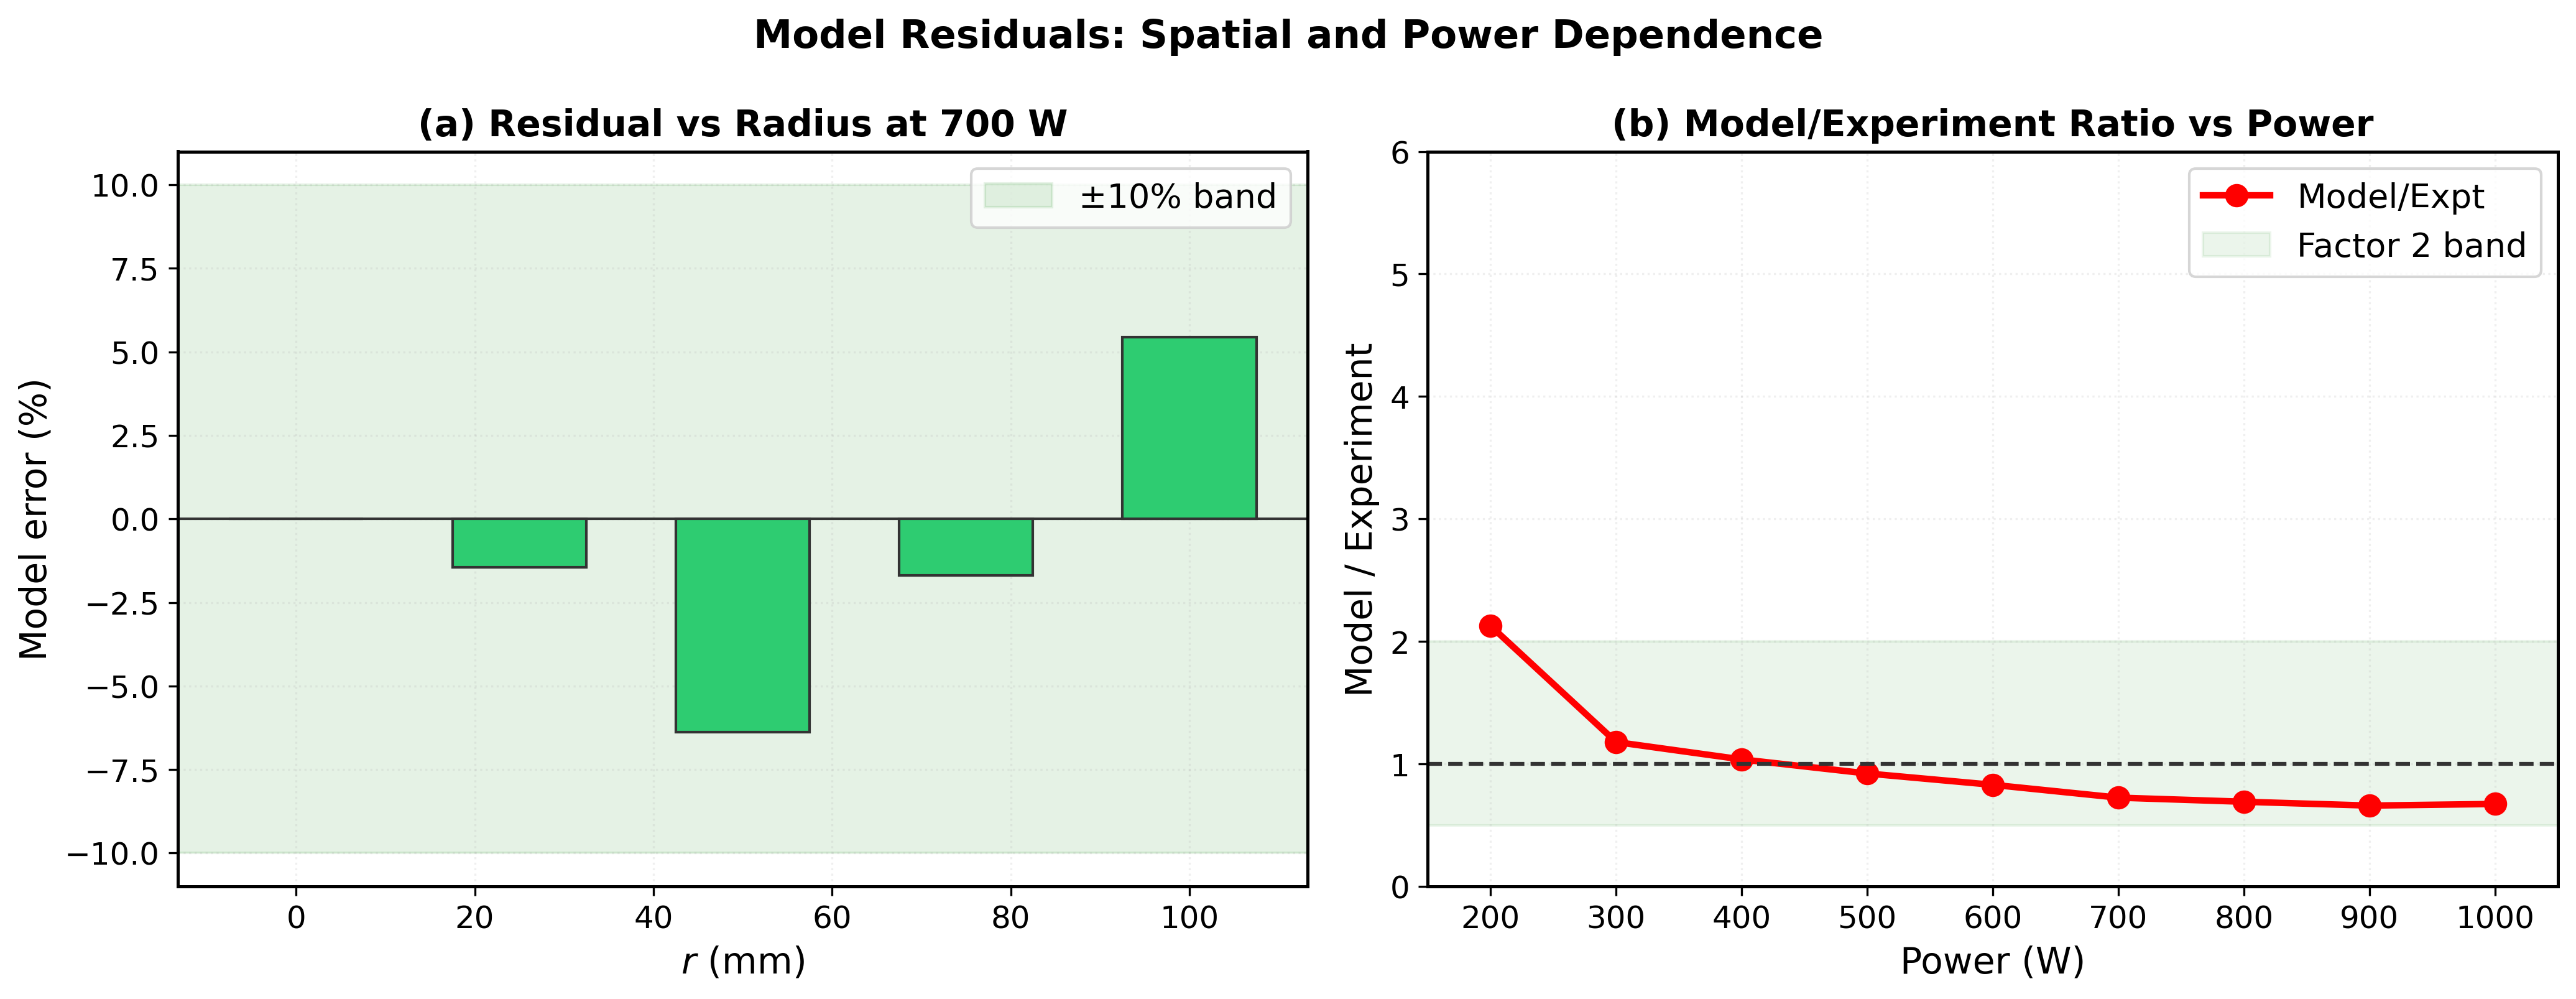
\includegraphics[width=0.85\linewidth]{residuals.png}\\
\small Residual distribution

\vspace{0.3em}
\small
Error uniform across all regions. No systematic over/underprediction.
\end{columns}
\end{frame}

% ----------------------------------------------------------
%  SLIDE 16 --- ML Baselines
% ----------------------------------------------------------
\begin{frame}{ML Baselines: Why a Tuned MLP?}
\centering
\begin{table}
\centering
\begin{tabular}{@{}lcl@{}}
\toprule
\textbf{Method} & \textbf{RMSE} & \textbf{Notes} \\
\midrule
Polynomial (degree 3)      & 0.051 & Severe underfitting \\
Polynomial (degree 4)      & 0.039 & Still underfits nonlinearities \\
Gaussian Process           & 0.006 & Good, but scales poorly with $N$ \\
\textbf{Our MLP (ensemble)} & \good{\textbf{0.0015}} & Fast inference, scalable \\
\bottomrule
\end{tabular}
\end{table}

\vspace{0.5em}
MLP achieves \hlnum{4$\times$} lower error than GP and \hlnum{26$\times$} lower than polynomial, while running in sub-millisecond inference time.
\end{frame}

% ----------------------------------------------------------
%  SLIDE 17 --- Speedup
% ----------------------------------------------------------
\begin{frame}{Inference Speedup}
\centering
\begin{table}
\centering
\begin{tabular}{@{}lcc@{}}
\toprule
\textbf{Solver} & \textbf{Time/case} & \textbf{Speedup} \\
\midrule
Legacy FD   & 7.8\,s & \good{\textbf{531$\times$}} \\
LXCat FD    & 14.4\,s & \good{\textbf{874$\times$}} \\
MLP surrogate & $<$1\,ms & --- \\
\bottomrule
\end{tabular}
\end{table}

\vspace{0.5em}
Enables $10^5$-point design sweeps in seconds.
\end{frame}

% ----------------------------------------------------------
%  SLIDE 18 --- Computational Cost
% ----------------------------------------------------------
\begin{frame}[shrink=5]{Computational Cost: 97 Hours of Training}
\small
\centering
\begin{table}
\centering
\footnotesize
\begin{tabular}{@{}llcl@{}}
\toprule
\textbf{Experiment} & \textbf{Runs} & \textbf{Hours} & \textbf{Key metric} \\
\midrule
\multicolumn{4}{@{}l}{\textbf{Core experiments (41.1\,h)}} \\
\quad Architecture sweep (E0--E6) & 21 & 11.4 & E3 wins: nF\,=\,0.00210 \\
\quad Ablation study & 15 & 21.8 & bias\_only: nF\,=\,0.00314 \\
\quad Production ensemble & 5 & 7.9 & nF\,=\,0.00154 \\
\midrule
\multicolumn{4}{@{}l}{\textbf{Supplementary experiments (53.6\,h)}} \\
\quad Transfer learning & 6 & 17.7 & No benefit \\
\quad Mixed-physics training & 3 & 19.4 & Hurts both regimes \\
\quad $T_e$ auxiliary head & 3 & 16.5 & Hurts nF by 11\% \\
\midrule
\multicolumn{4}{@{}l}{\textbf{Fast validation (2.7\,h)}} \\
\quad ML baselines + mesh + speedup + spatial + lit + diag & --- & 2.7 & All passed \\
\bottomrule
\end{tabular}
\end{table}

\vspace{0.3em}
Supplementary experiments (\bad{all negative}) consumed \hlnum{55\%} of total compute---but preemptively answer reviewer questions.\\
All training on Apple MPS (GPU) or CPU; multiple experiments ran in parallel.
\end{frame}

% ----------------------------------------------------------
%  SLIDE 19 --- What Mattered Most
% ----------------------------------------------------------
\begin{frame}[shrink=5]{What Mattered Most (Ranked)}
\small
\begin{enumerate}\setlength\itemsep{2pt}
    \item \textbf{Bias initialisation to physical mean} --- \hlnum{83\%} of the gain; single most important trick
    \item \textbf{Separate per-species heads (E3)} --- \hlnum{89\%} reduction vs.\ vanilla; captures distinct density scales
    \item \textbf{Physics regularisation} --- \bad{useless}; adds 3\% \emph{more} error
    \item \textbf{Cosine-annealing LR schedule} --- 12\% gain; helpful but secondary
    \item \textbf{Ensemble averaging} --- additional 47\% over single model
    \item \textbf{Data source (LXCat vs.\ legacy)} --- \bad{irrelevant}; statistically identical
\end{enumerate}

\vspace{0.5em}
\centering
\fbox{\textbf{Lesson:} Training recipe dominates architecture, which dominates data source.}
\end{frame}

% ----------------------------------------------------------
%  SLIDE 19 --- Limitations
% ----------------------------------------------------------
\begin{frame}{Limitations \& Caveats}
\small
\begin{itemize}\setlength\itemsep{2pt}
    \item \textbf{F density:} solver shows \bad{36\% error} vs.\ literature --- surrogate inherits this ceiling
    \item \textbf{LXCat $T_e$:} \bad{58\% error} vs.\ experimental data; legacy is better at 5\%
    \item \textbf{2D only:} axisymmetric geometry; no 3D asymmetries captured
    \item \textbf{Steady-state:} no transient dynamics (ignition, pulsed plasmas)
    \item \textbf{Fixed geometry:} no shape generalisation --- retrain needed for new reactors
    \item Ensemble spread used as uncertainty proxy --- not a calibrated Bayesian posterior
\end{itemize}
\end{frame}

% ----------------------------------------------------------
%  SLIDE 20 --- Next Steps
% ----------------------------------------------------------
\begin{frame}{Next Steps}
\begin{columns}[T]
\column{0.55\textwidth}
\small
\begin{enumerate}\setlength\itemsep{0pt}
    \item \textbf{Phase 2:} BOLSIG+ EEDF $\to$ PINN Boltzmann $\to$ PIC-MCC validation
    \item \textbf{3D extension:} graph neural network or DeepONet
    \item \textbf{Transient rollout:} neural ODE for pulsed plasmas
    \item \textbf{Experimental validation:} wafer-level etch measurements
\end{enumerate}
\column{0.42\textwidth}
\centering
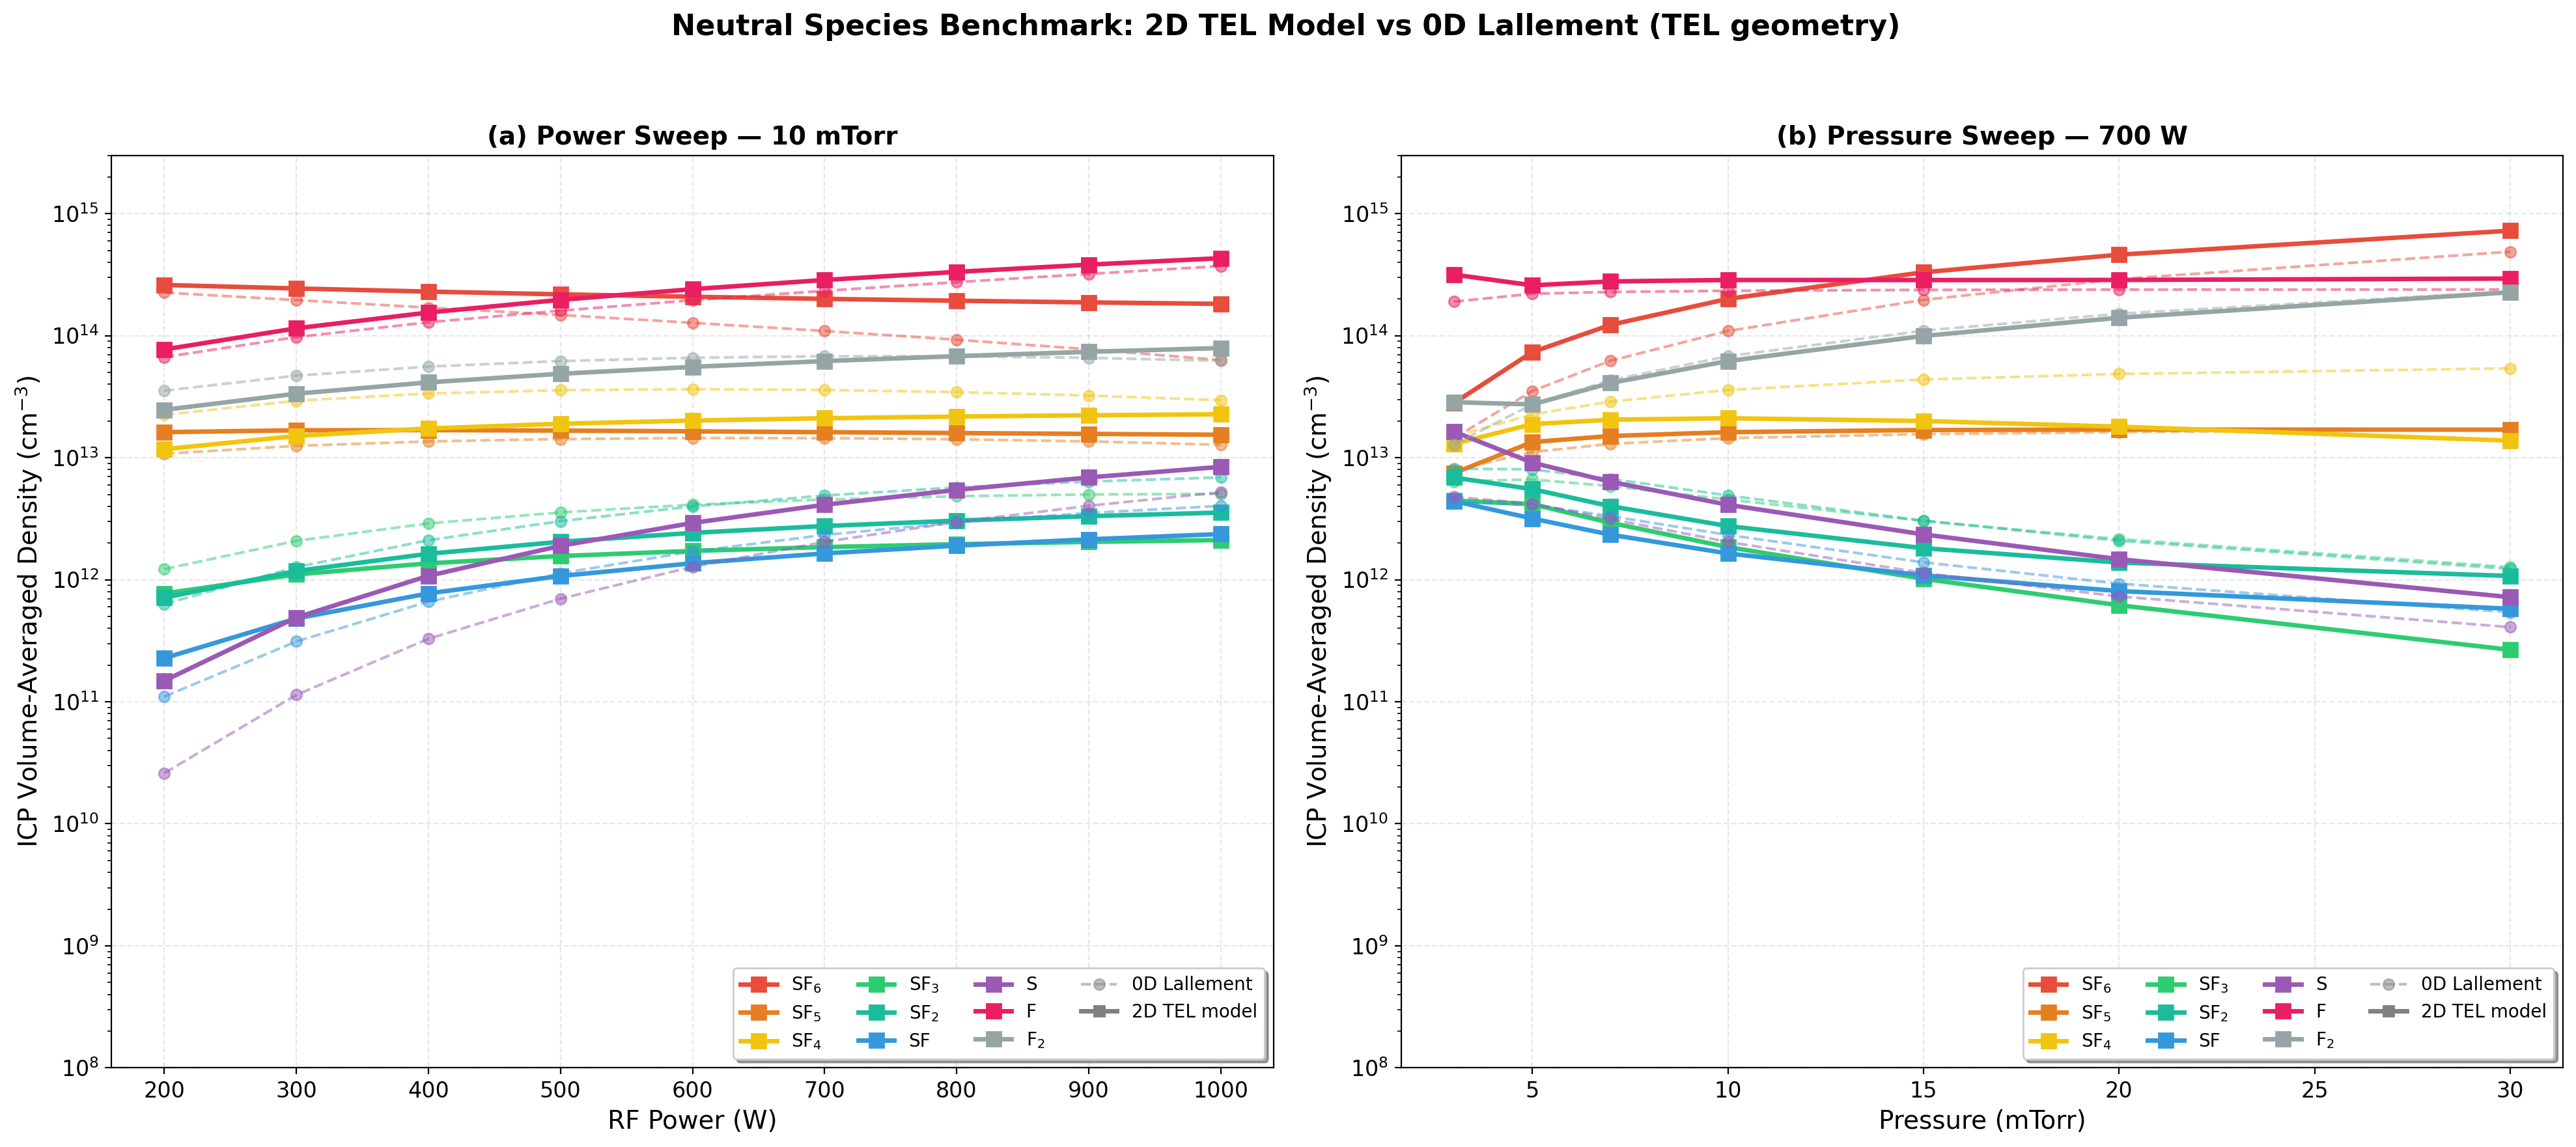
\includegraphics[width=0.85\linewidth]{benchmark_neutrals.png}\\
\small Neutral benchmark
\end{columns}
\end{frame}

% ----------------------------------------------------------
%  SLIDE 21 --- Conclusion
% ----------------------------------------------------------
\begin{frame}[shrink=5]{Conclusion}
\small
\textbf{Since our last meeting}, three directions explored:

\vspace{0.3em}
\begin{enumerate}\setlength\itemsep{2pt}
    \item \textbf{PINN:} PDE-constrained approach \bad{fails} for stiff multi-species plasma chemistry. Data-only PINN converges but is 23\,000$\times$ slower --- no benefit.

    \item \textbf{Supervised MLP surrogate:} Fourier features + separate heads + bias initialisation achieves \good{RMSE = 0.00154} ($n_F$), a \hlnum{531--874$\times$} speedup, and \hlnum{47\%} improvement over single-model v4.

    \item \textbf{LXCat integration:} Biagi cross sections shift $T_e$ and $n_e$ dramatically, but the surrogate gap was \textbf{training recipe}, not data source.
\end{enumerate}

\vspace{0.3em}
\centering
\fbox{\textbf{Key insight:} Bias init $>$ architecture $>$ data source. Recipe is everything.}
\end{frame}

% ============================================================
%  BACKUP SLIDES
% ============================================================
\appendix

\begin{frame}[standout]
Backup Slides
\end{frame}

% ----------------------------------------------------------
%  BACKUP 1 --- PINN Failure Details
% ----------------------------------------------------------
\begin{frame}{Backup: PINN Failure --- Detailed Analysis}
\begin{columns}[T]
\column{0.50\textwidth}
\small
\textbf{PDE-constrained PINN}
\begin{itemize}\setlength\itemsep{0pt}
    \item 54 coupled species as soft constraints
    \item Stiff chemistry defeats gradient descent
    \item Adaptive loss weighting cannot help
\end{itemize}
\column{0.50\textwidth}
\small
\textbf{Data-only PINN}
\begin{itemize}\setlength\itemsep{0pt}
    \item Converges, but \hlnum{23\,000$\times$} slower
    \item No accuracy gain over plain MLP
    \item Physics loss is counterproductive here
\end{itemize}
\end{columns}
\vspace{0.2em}
\centering
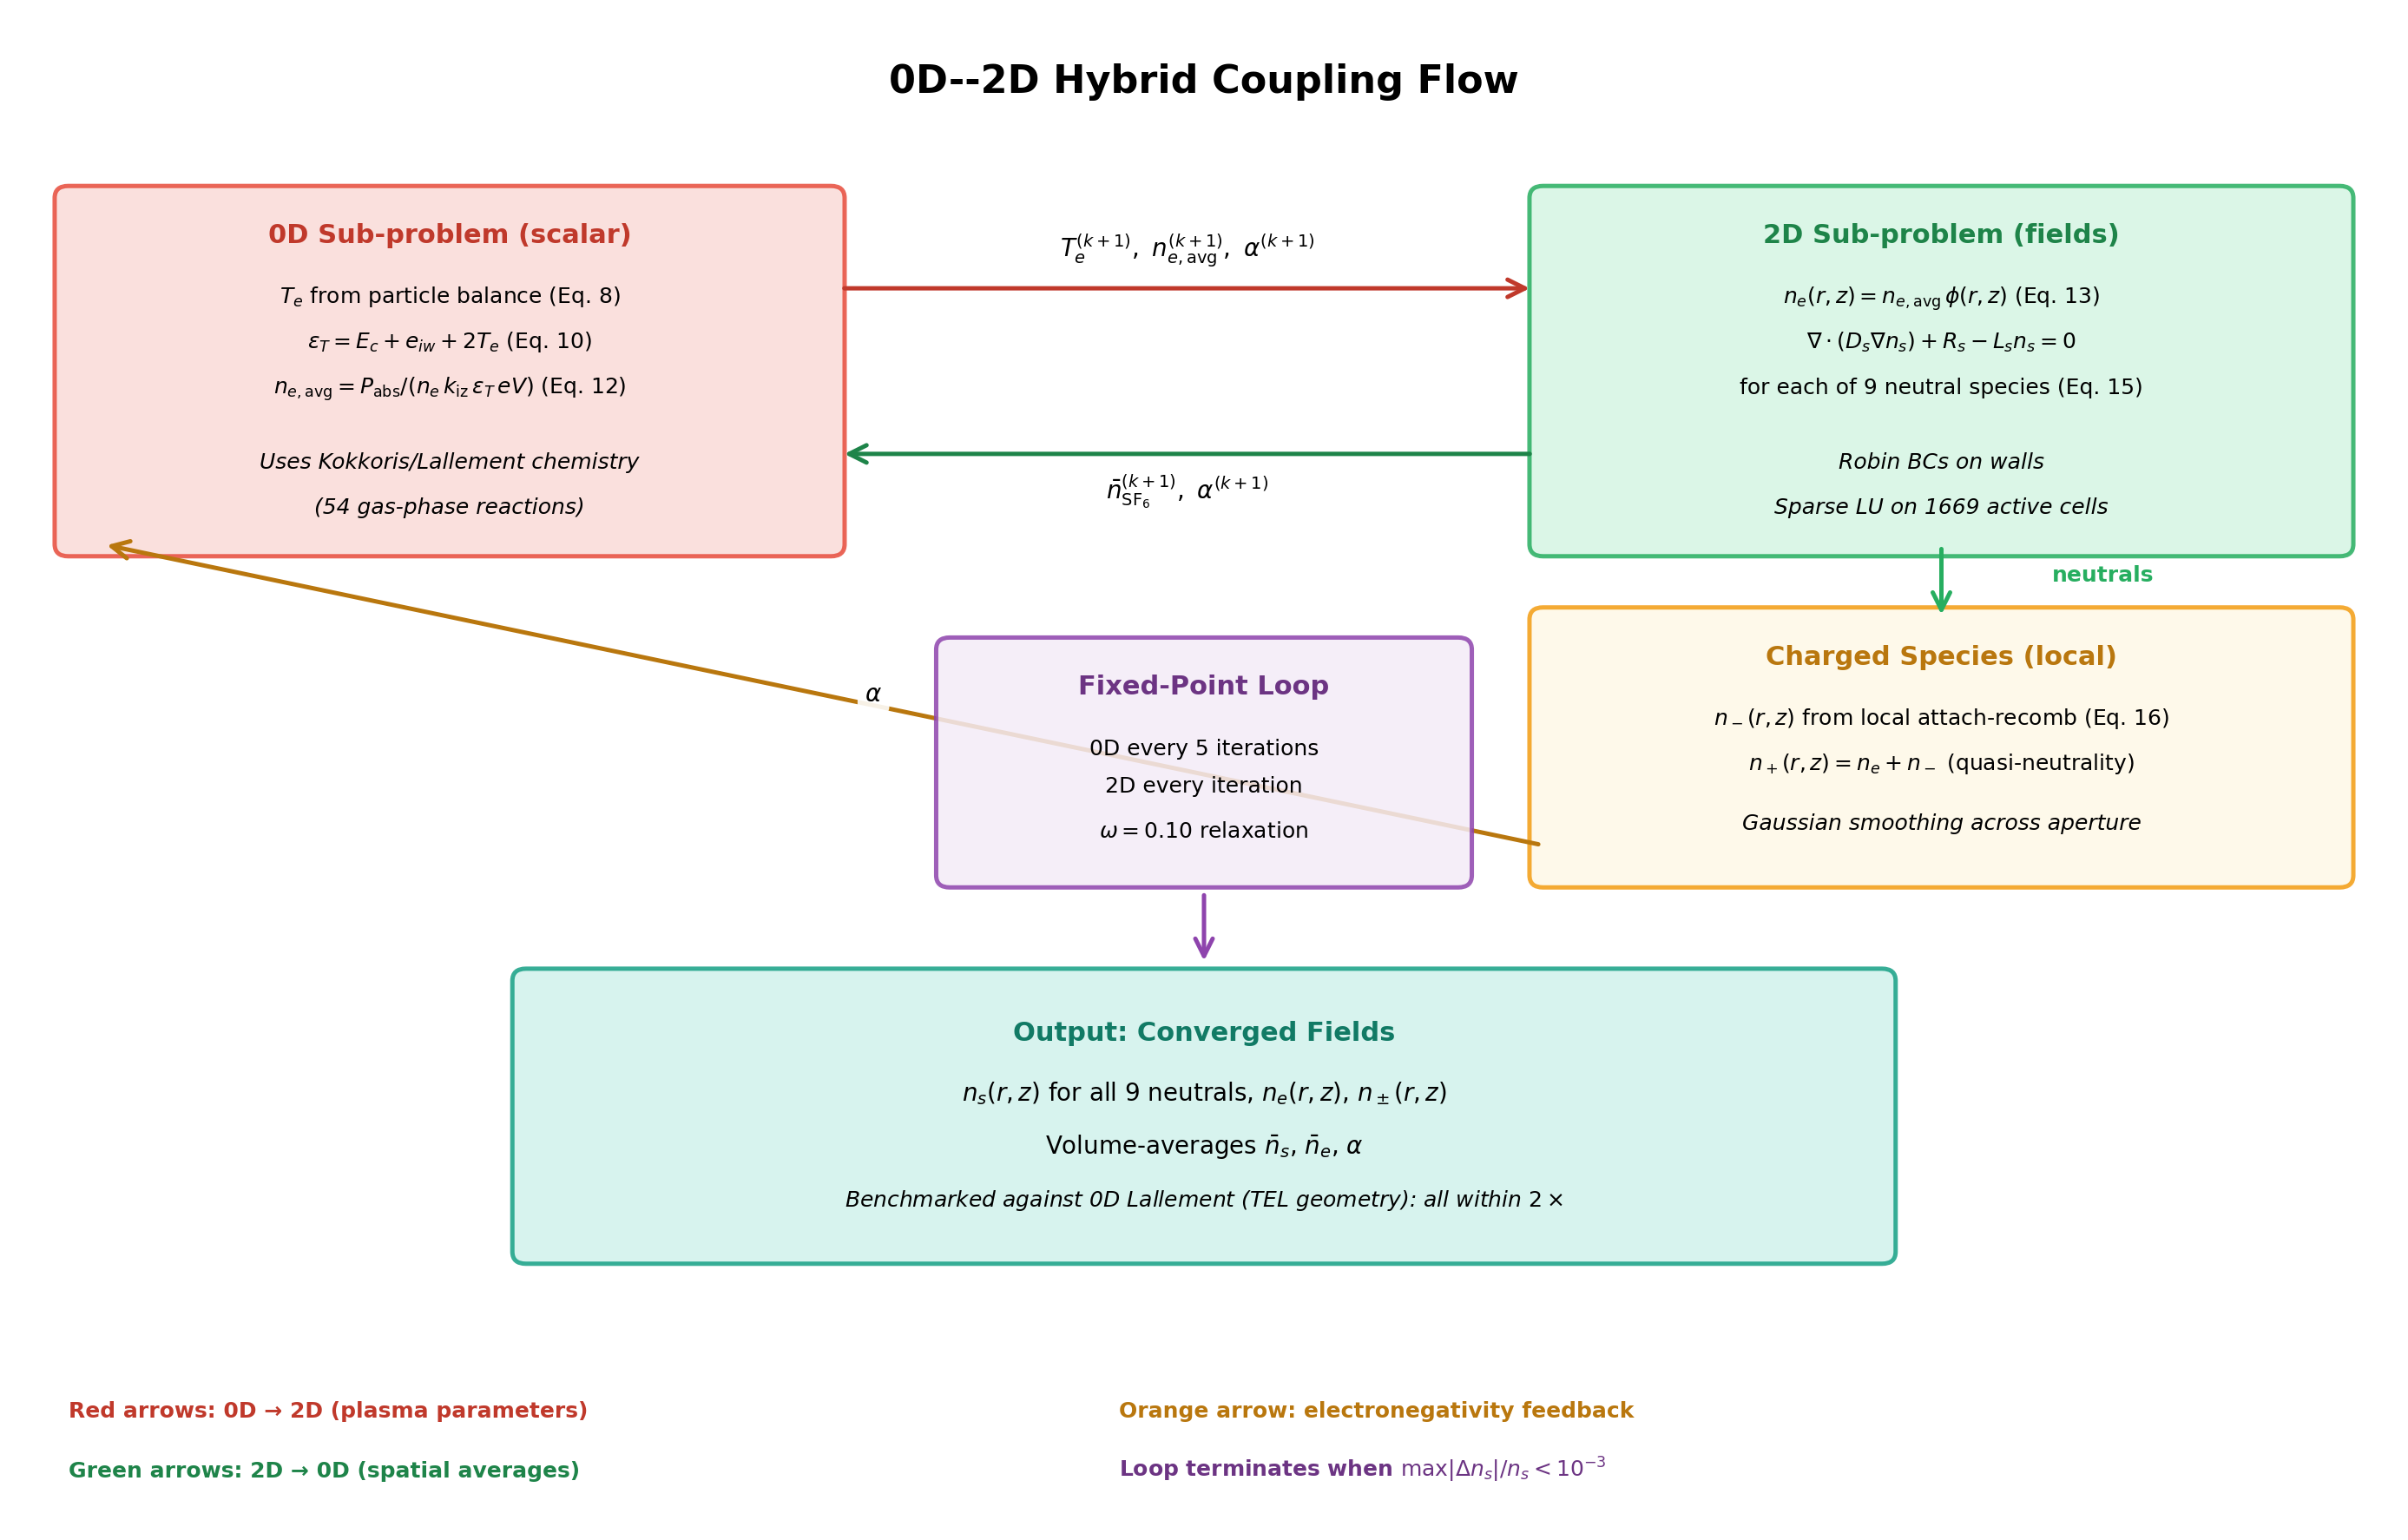
\includegraphics[width=0.4\linewidth]{coupling_flowchart.png}
\end{frame}

% ----------------------------------------------------------
%  BACKUP 2 --- Transfer Learning
% ----------------------------------------------------------
\begin{frame}[shrink=3]{Backup: Transfer Learning --- No Benefit}
\begin{columns}[T]
\column{0.50\textwidth}
\textbf{Strategy}
\begin{itemize}
    \item Pre-train on legacy dataset
    \item Fine-tune on LXCat dataset
    \item Hypothesis: domain adaptation should help
\end{itemize}

\vspace{0.5em}
\textbf{Result: \bad{No benefit}}
\begin{itemize}
    \item Datasets too similar for transfer to add value
    \item From-scratch training matches or beats fine-tuning
    \item Confirms the ``statistically identical'' finding
\end{itemize}
\column{0.48\textwidth}
\centering
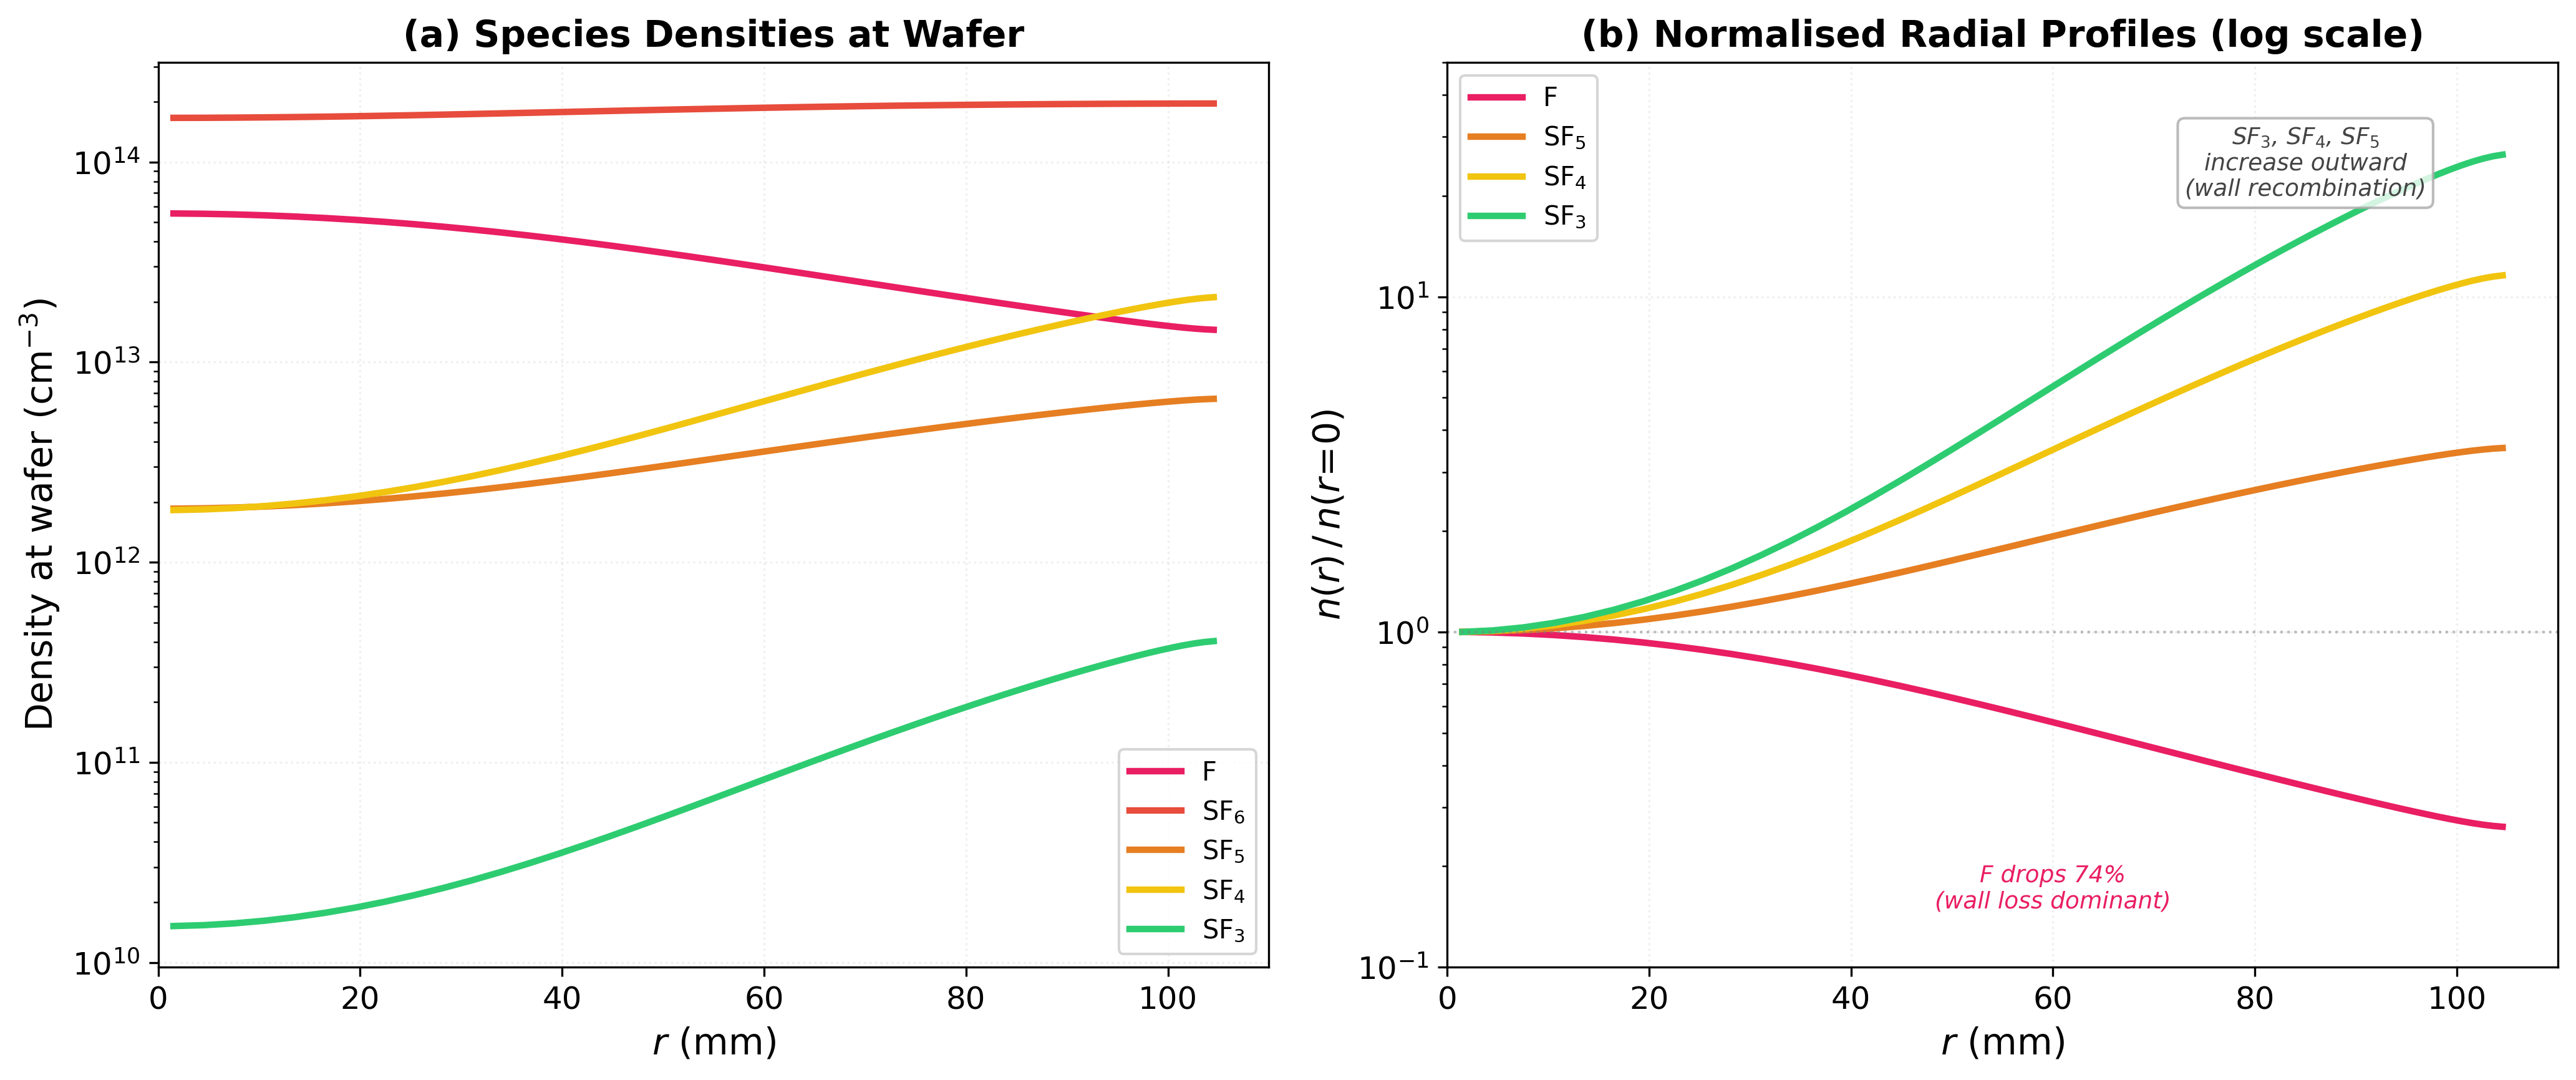
\includegraphics[width=\linewidth]{multispecies_radial.png}\\
\small Radial profiles: legacy vs.\ LXCat overlap
\end{columns}
\end{frame}

% ----------------------------------------------------------
%  BACKUP 3 --- Te Auxiliary Head
% ----------------------------------------------------------
\begin{frame}[shrink=3]{Backup: $T_e$ Auxiliary Head --- Hurts $n_F$}
\begin{columns}[T]
\column{0.50\textwidth}
\textbf{Multi-task approach}
\begin{itemize}
    \item Predict $T_e$ alongside species densities
    \item Idea: shared representation should help
    \item Result: \bad{$n_F$ RMSE increases by 11\%}
    \item Gradient interference between density and temperature tasks
\end{itemize}
\column{0.50\textwidth}
\centering
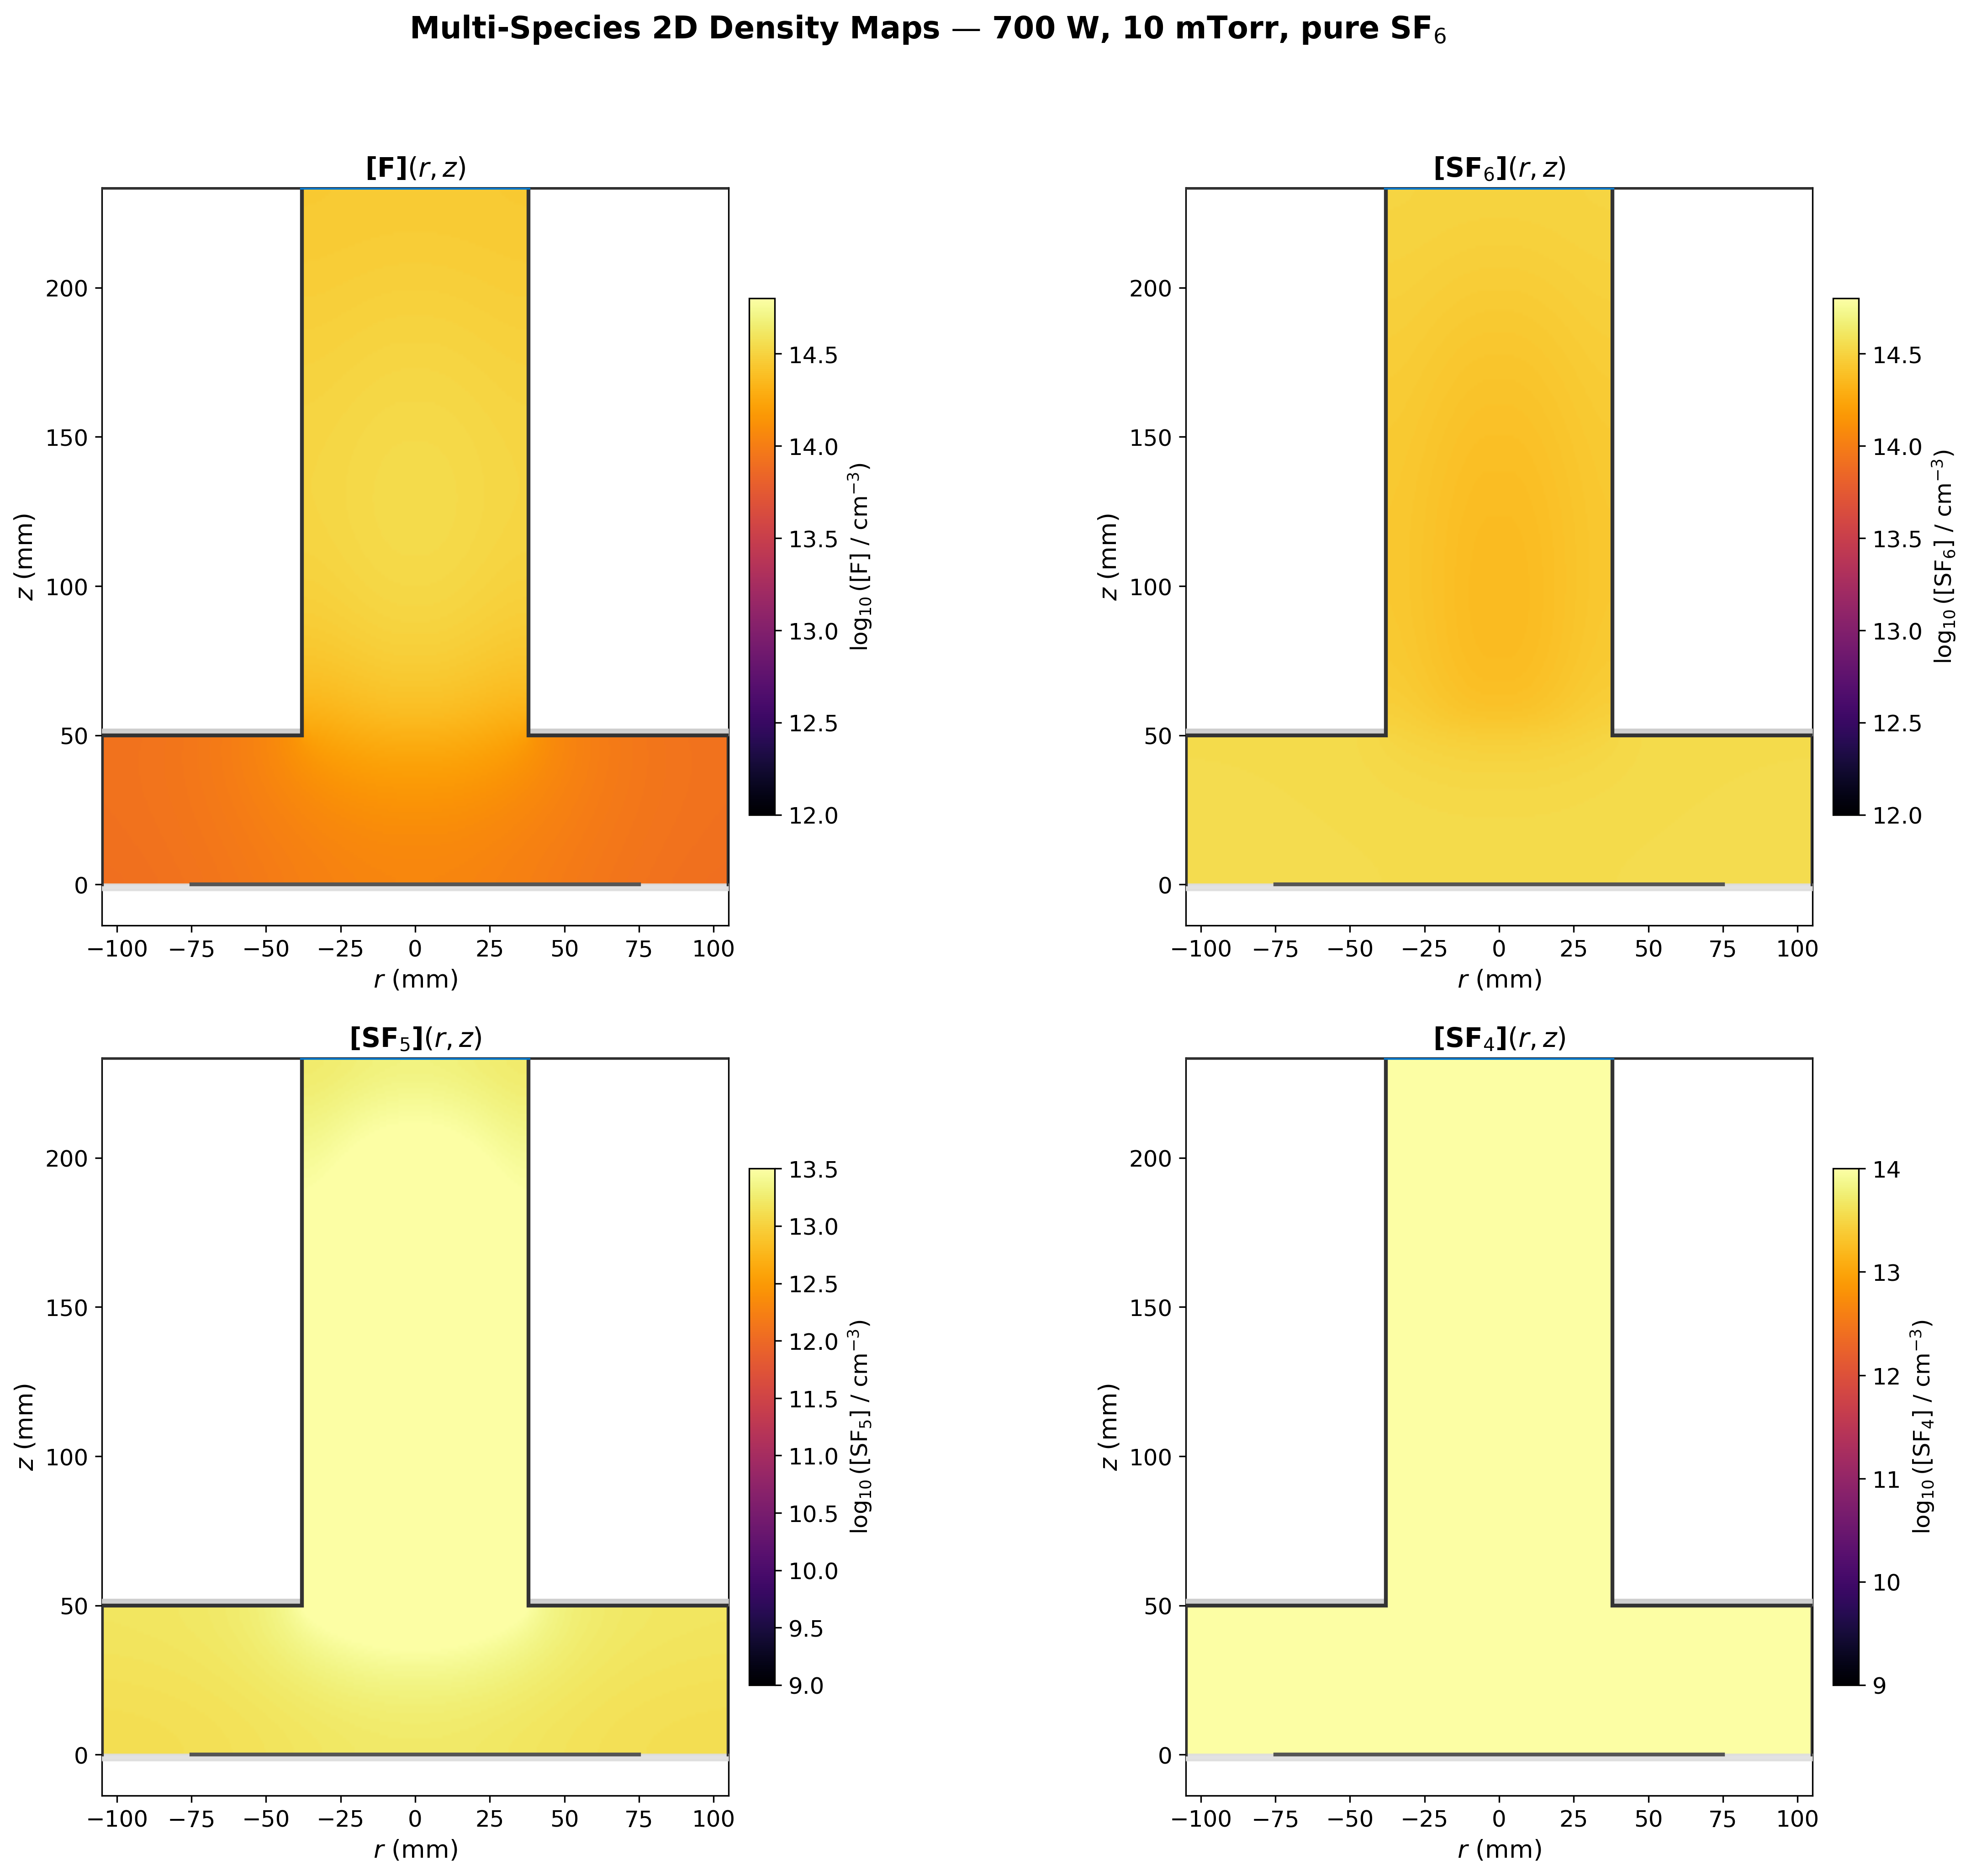
\includegraphics[width=\linewidth]{multispecies_contours.png}\\
\small Multi-species density contours
\end{columns}
\end{frame}

% ----------------------------------------------------------
%  BACKUP 4 --- Mixed-Physics Training
% ----------------------------------------------------------
\begin{frame}[shrink=3]{Backup: Mixed-Physics Training --- Fails}
\begin{columns}[T]
\column{0.50\textwidth}
\textbf{Strategy}
\begin{itemize}
    \item Combine legacy + LXCat regime data in one model
    \item Add regime indicator as input feature
\end{itemize}

\vspace{0.5em}
\textbf{Result: \bad{2--6$\times$ worse} in both regimes}
\begin{itemize}
    \item Conflicting physics confuses the shared trunk
    \item Regime indicator insufficiently separates the manifolds
    \item Separate models remain superior
\end{itemize}
\column{0.48\textwidth}
\centering
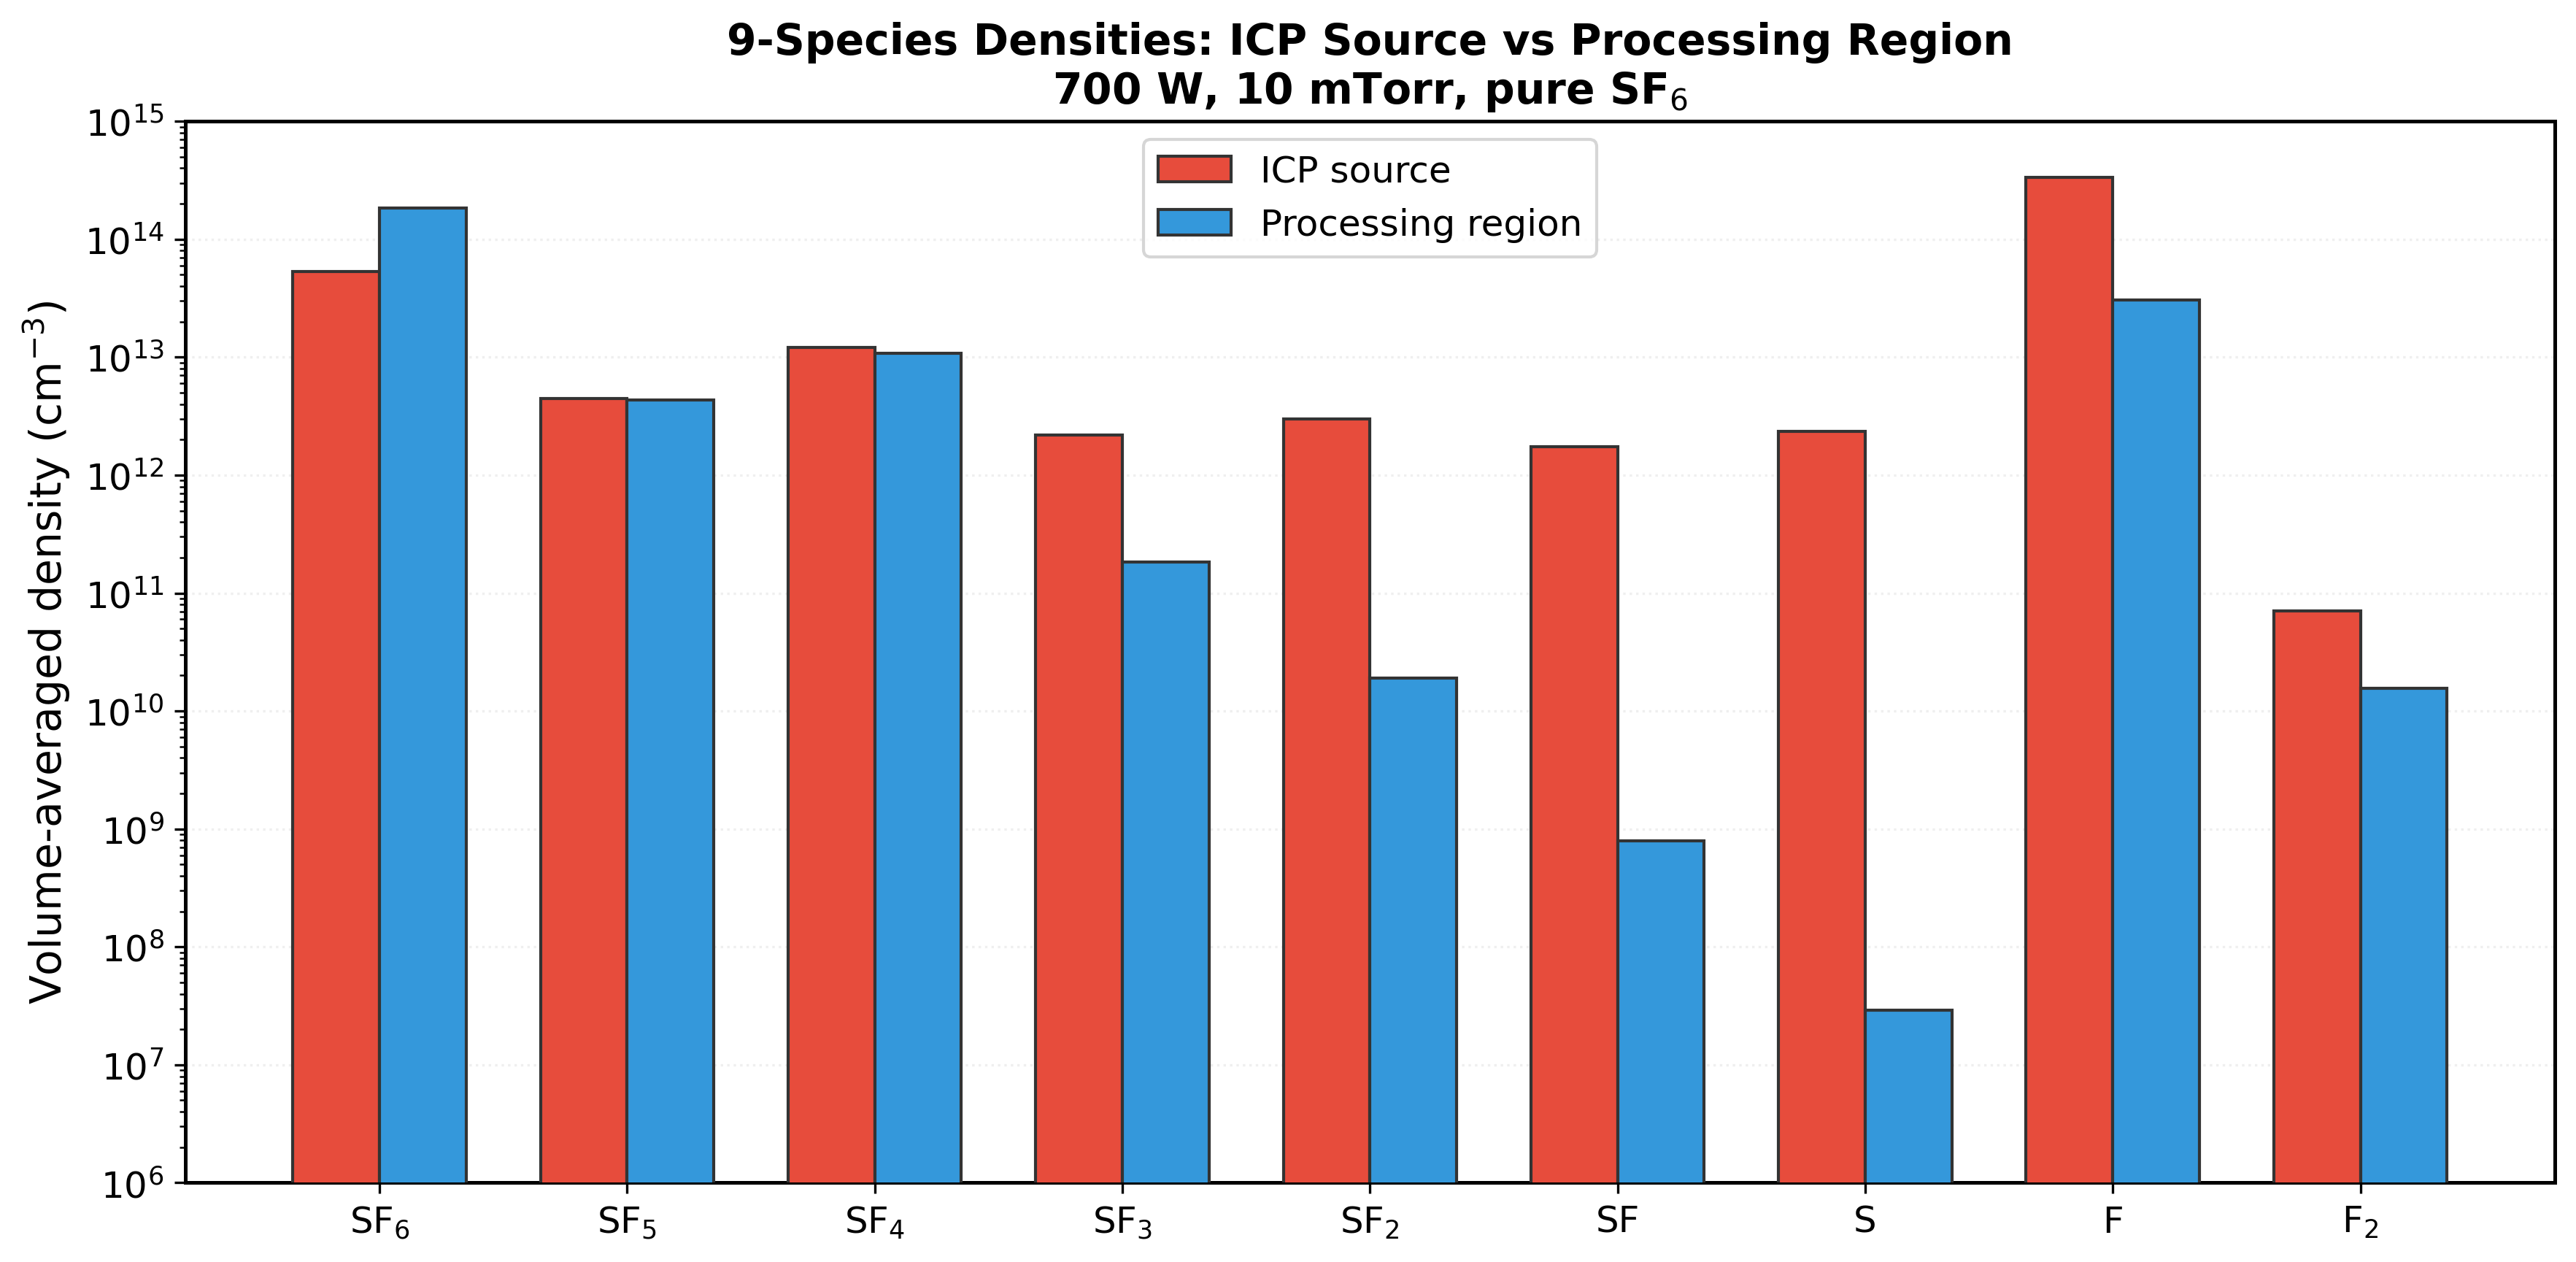
\includegraphics[width=\linewidth]{multispecies_bars.png}\\
\small Species density comparison across regimes
\end{columns}
\end{frame}

% ----------------------------------------------------------
%  BACKUP 5 --- Multispecies Contours
% ----------------------------------------------------------
\begin{frame}[shrink=10]{Backup: Multi-Species Density Contours}
\centering
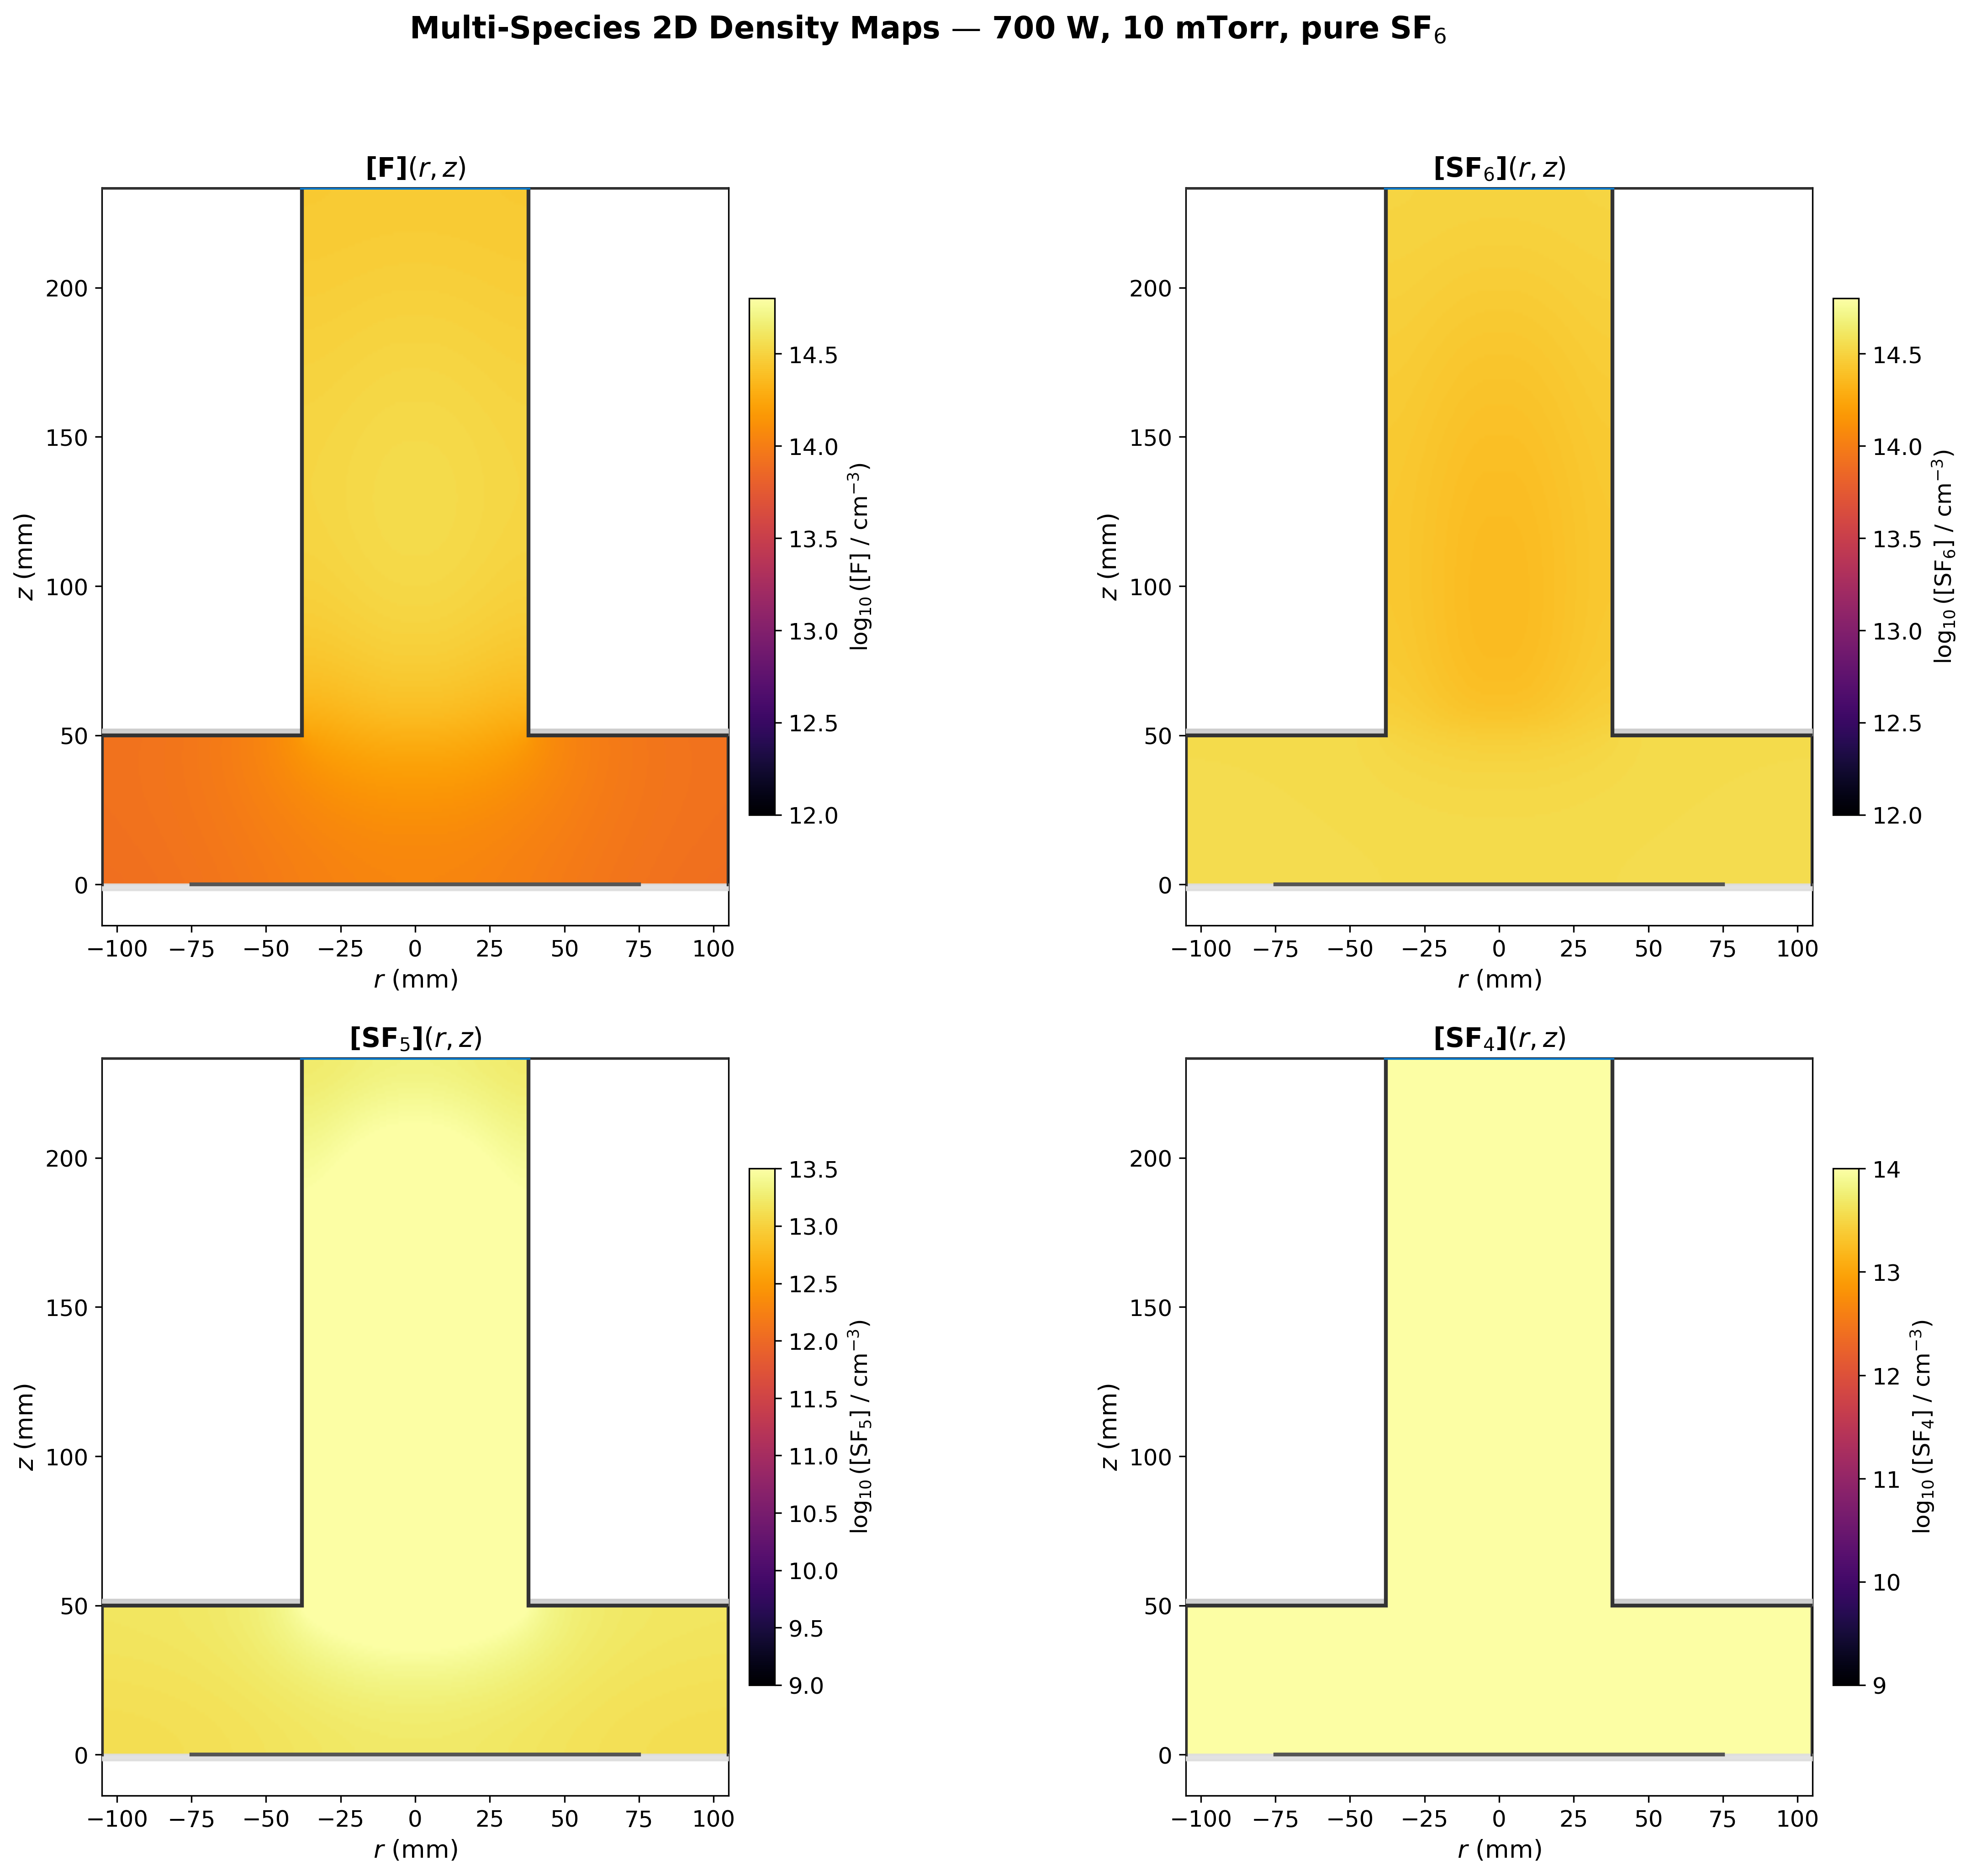
\includegraphics[width=0.78\linewidth]{multispecies_contours.png}

\vspace{0.3em}
Steady-state density contours for key species across the reactor cross-section.
\end{frame}

% ----------------------------------------------------------
%  BACKUP 6 --- Power Sweeps
% ----------------------------------------------------------
\begin{frame}{Backup: Power Sweep Validation}
\begin{columns}[T]
\column{0.48\textwidth}
\centering
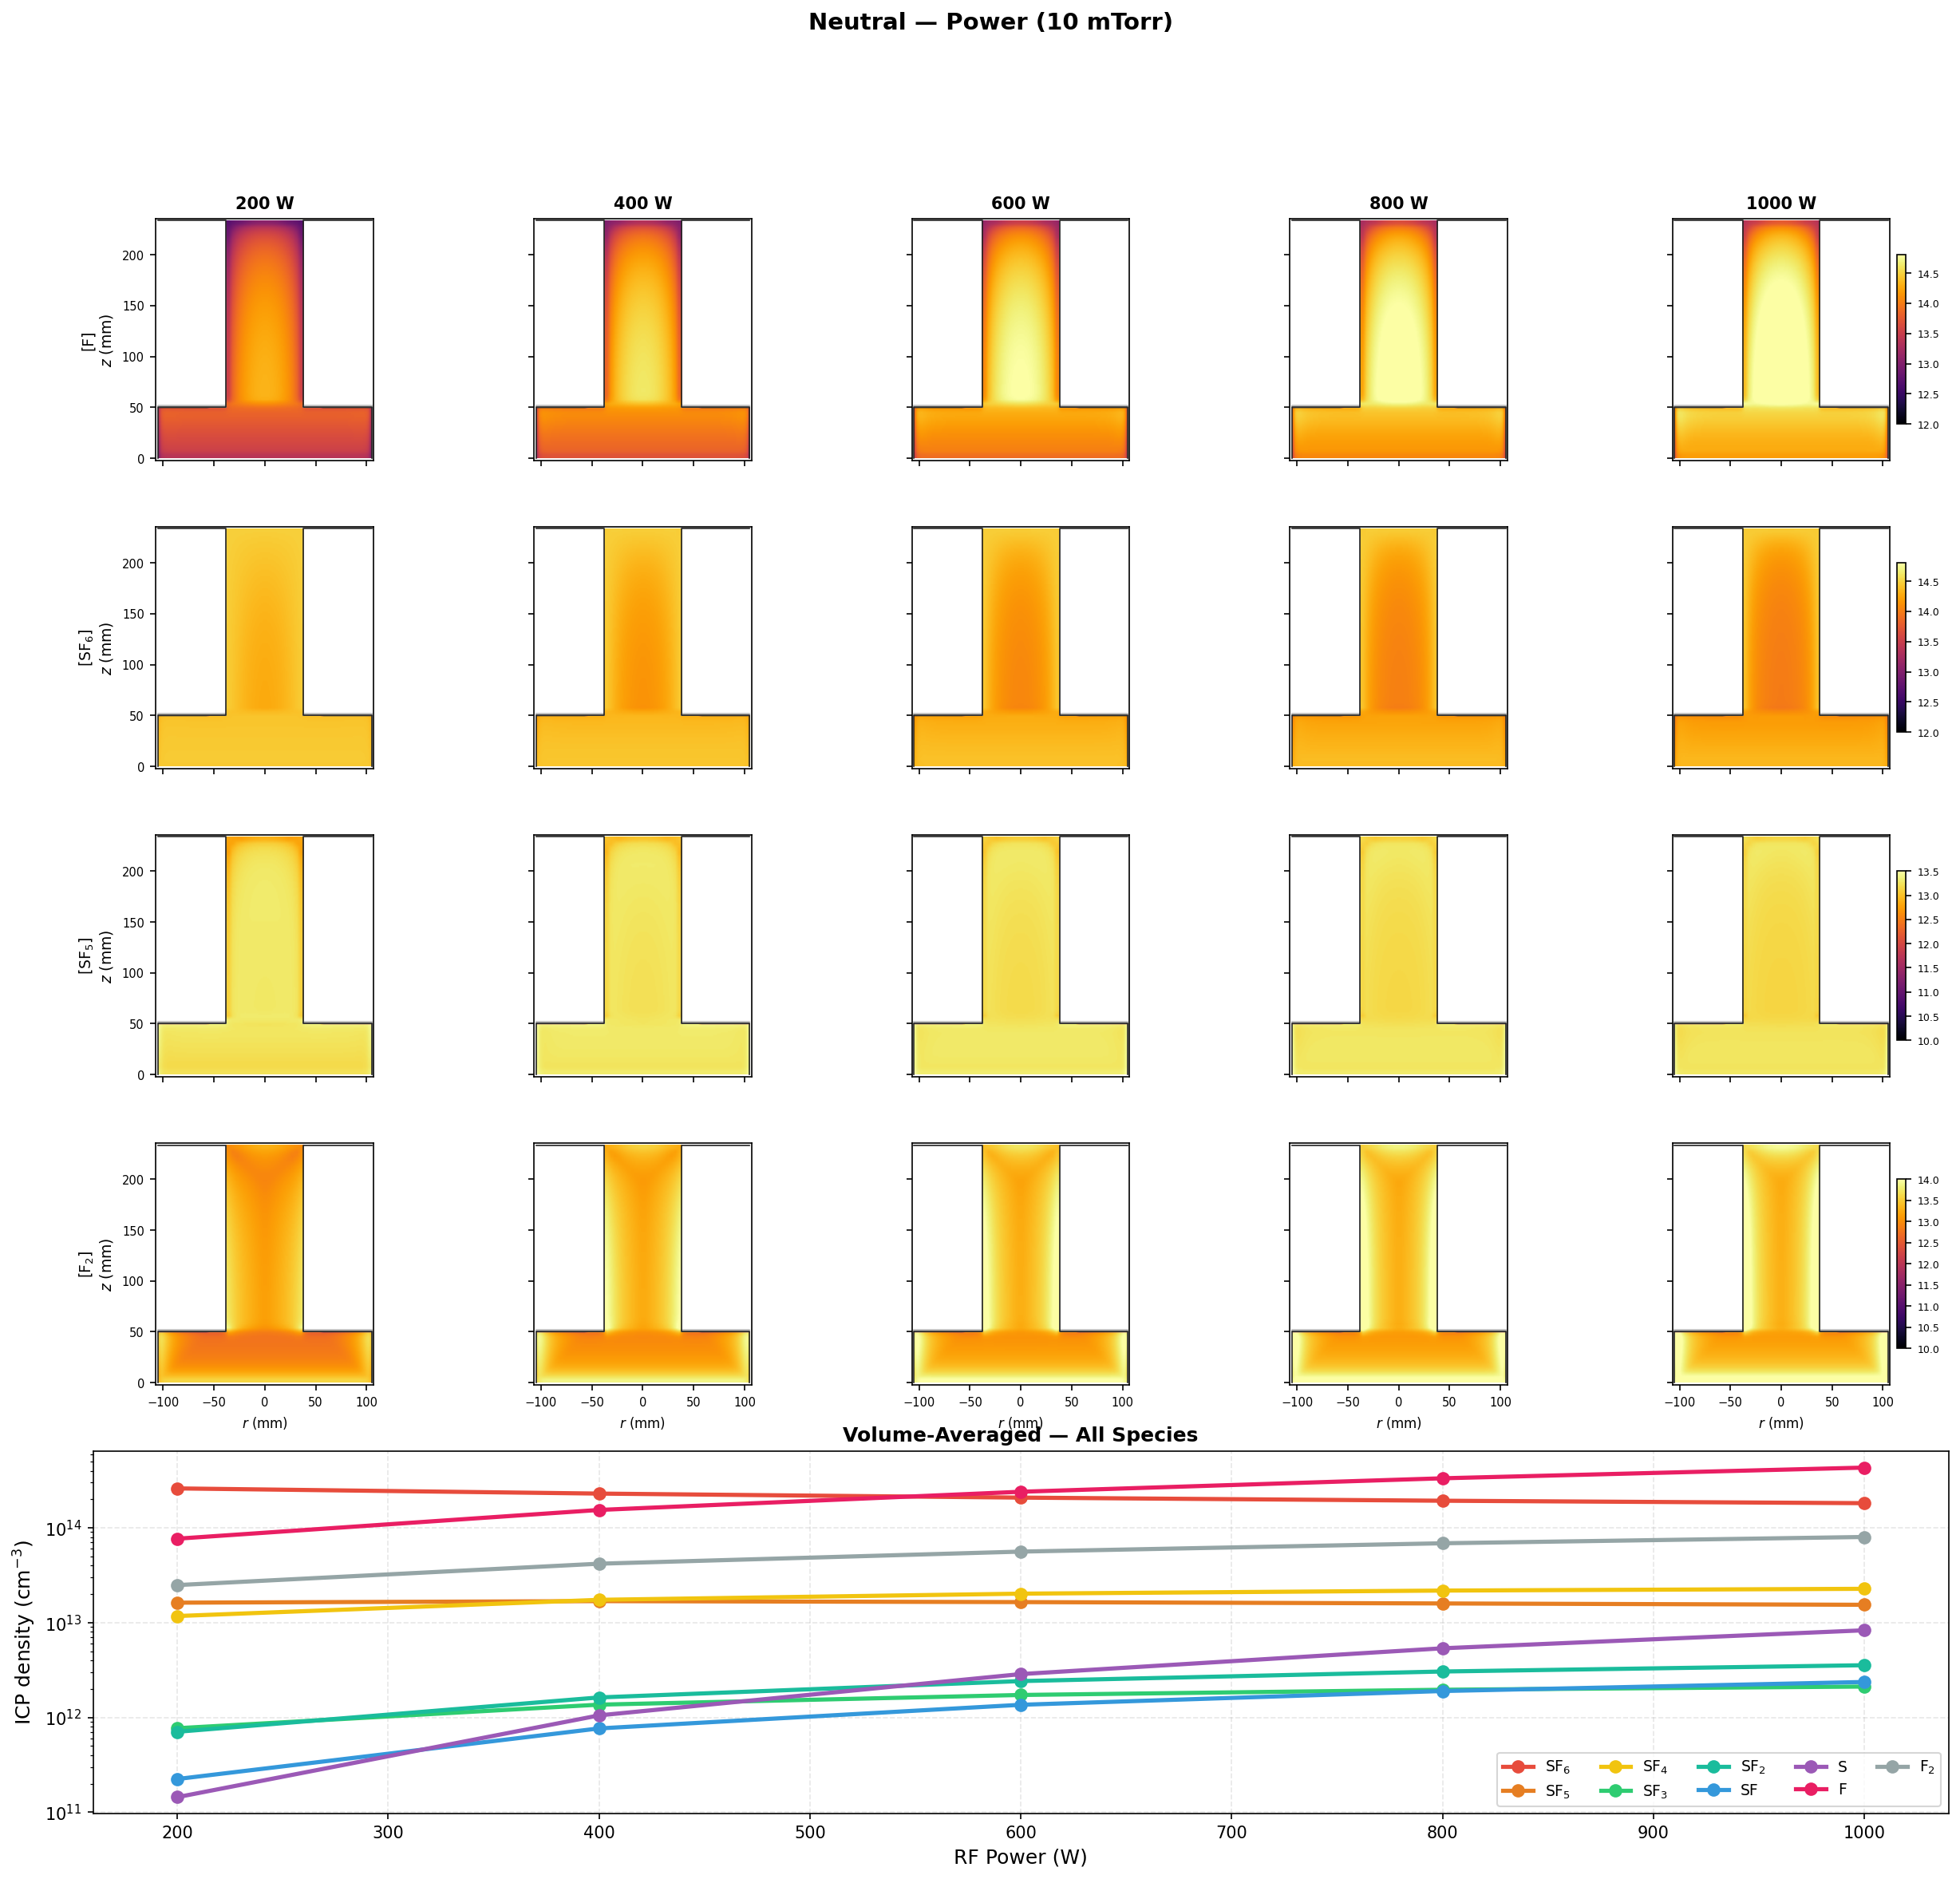
\includegraphics[width=0.85\linewidth]{neutral_power_2D.png}\\
\small Neutral species vs power
\column{0.48\textwidth}
\centering
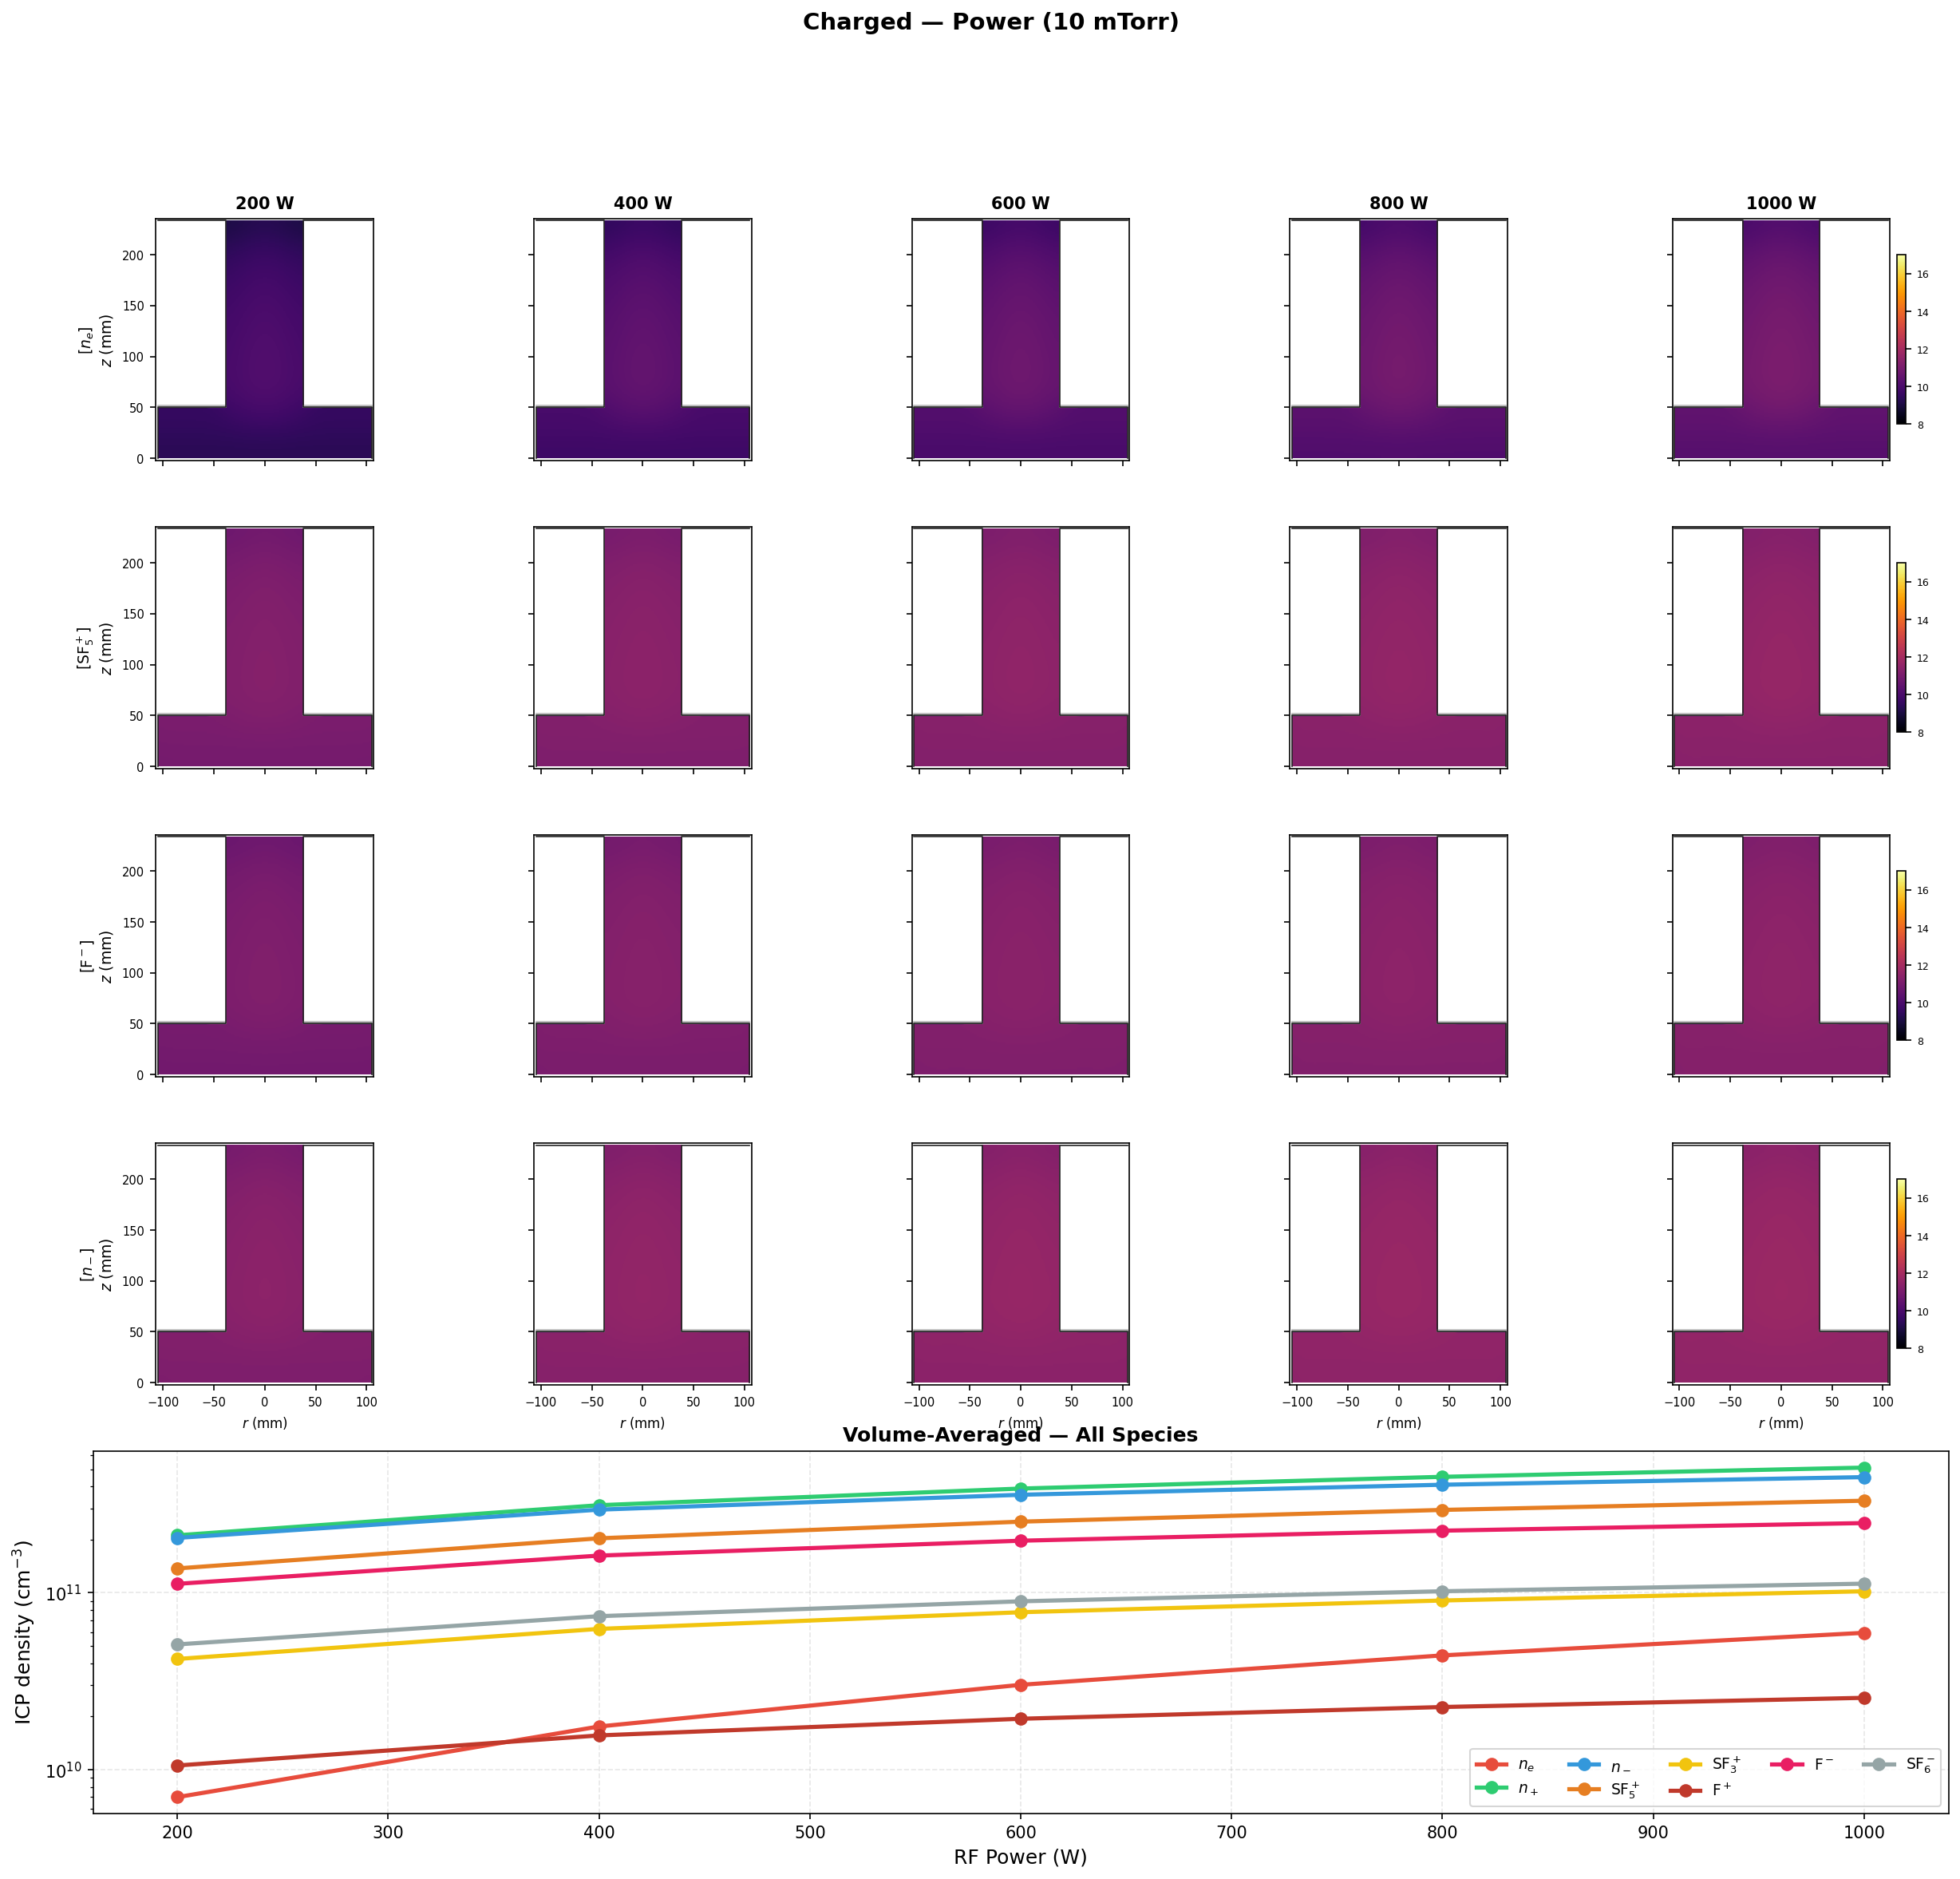
\includegraphics[width=0.85\linewidth]{charged_power_2D.png}\\
\small Charged species vs power
\end{columns}
\end{frame}

% ----------------------------------------------------------
%  BACKUP 7 --- Composition Sweep
% ----------------------------------------------------------
\begin{frame}{Backup: Composition Sweep}
\centering
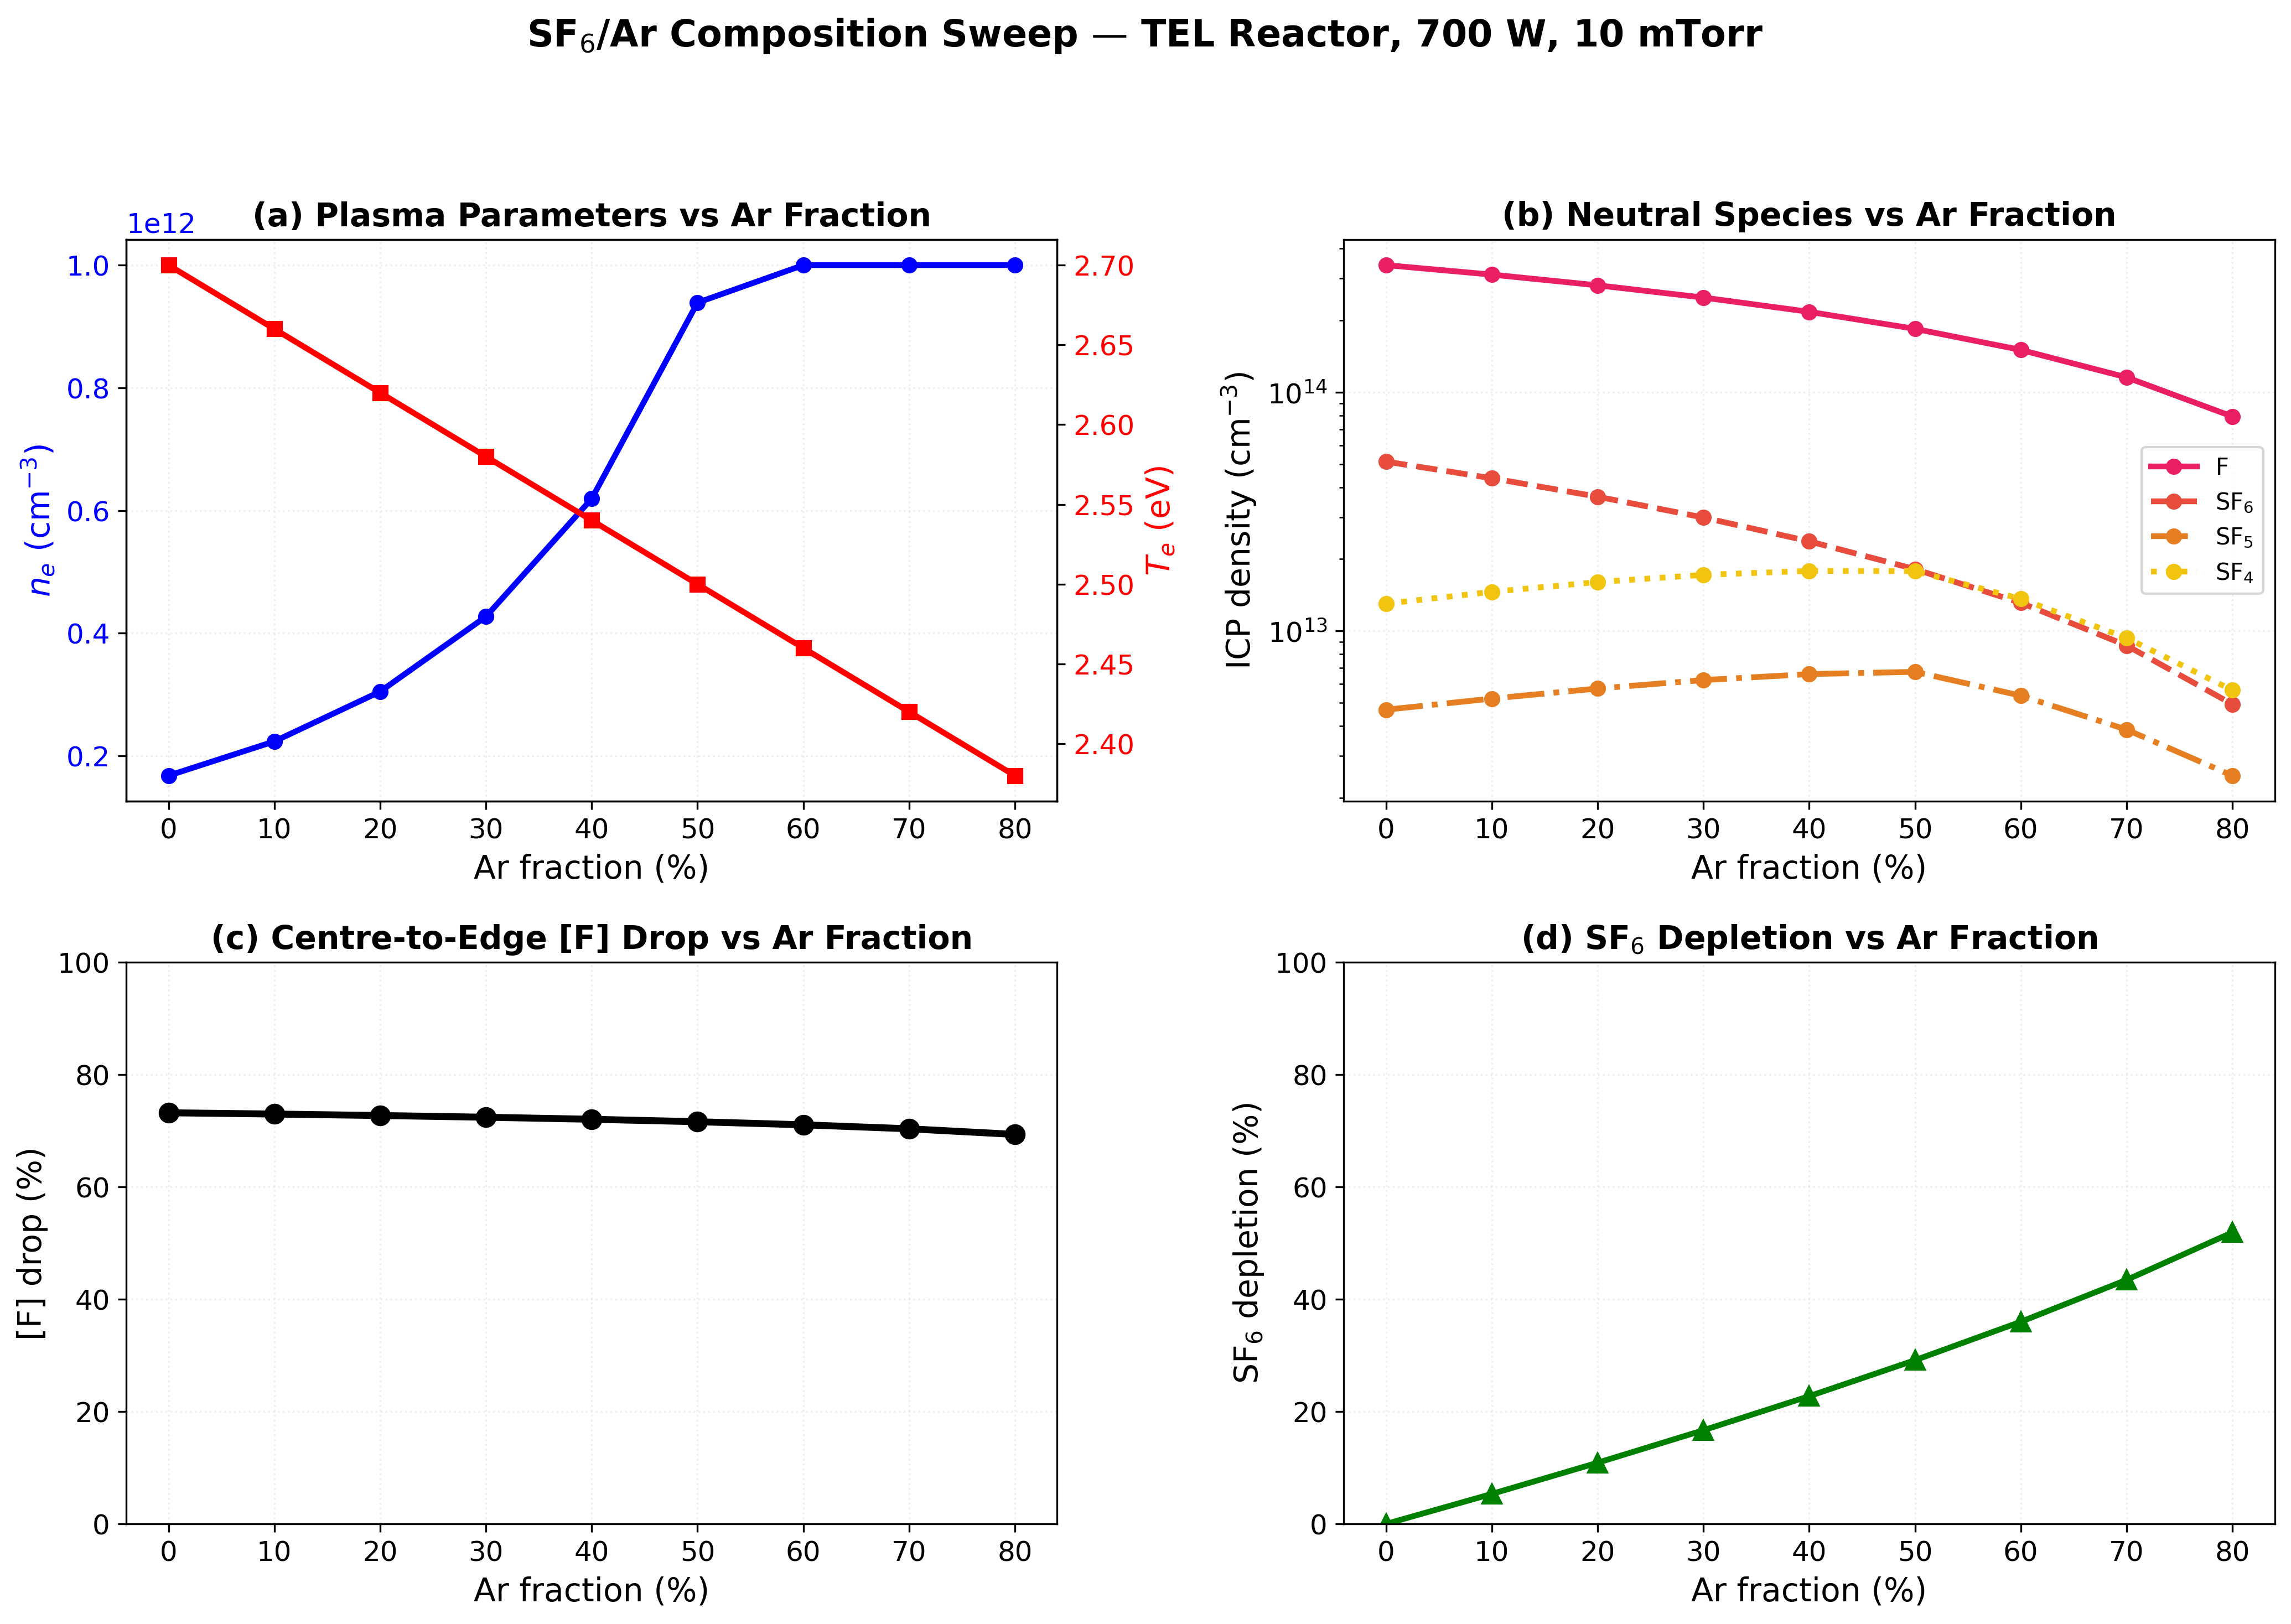
\includegraphics[width=0.72\linewidth]{composition_sweep.png}

\vspace{0.3em}
Surrogate faithfully reproduces the non-monotonic SF\textsubscript{6}/Ar composition dependence seen in the full solver.
\end{frame}

% ----------------------------------------------------------
%  BACKUP 8 --- Sensitivity Map
% ----------------------------------------------------------
\begin{frame}{Backup: Input Sensitivity Analysis}
\centering
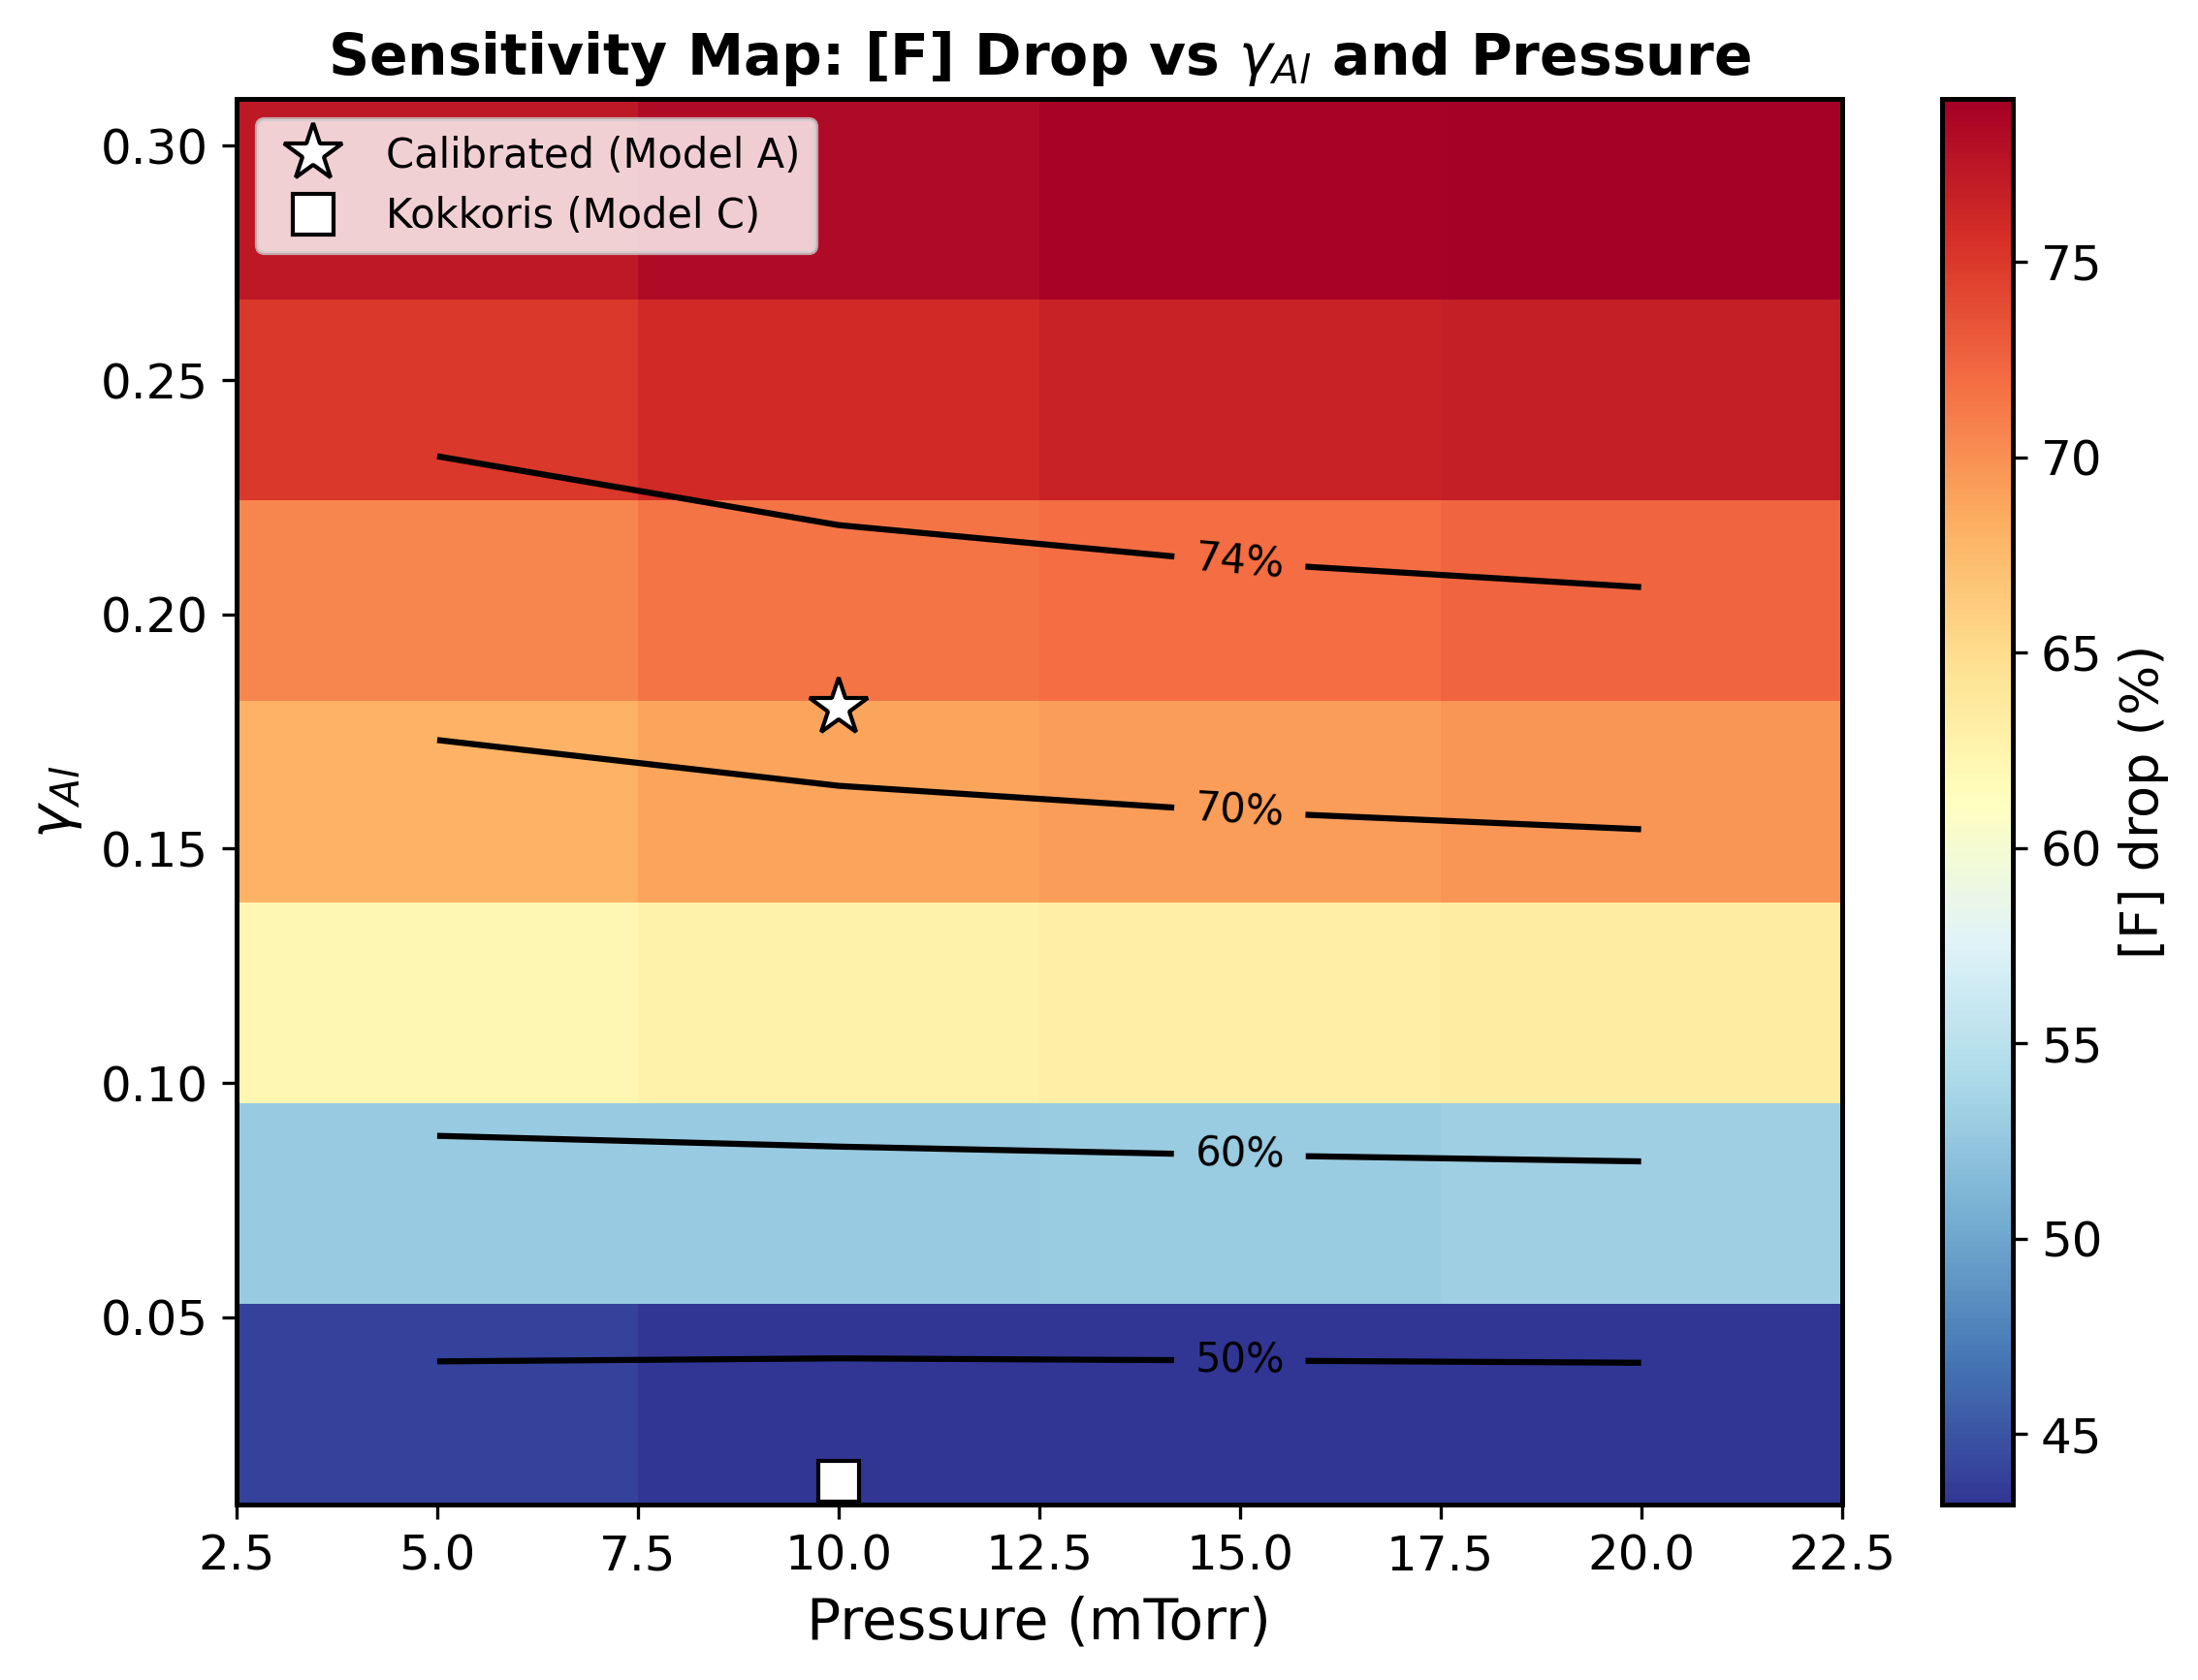
\includegraphics[width=0.60\linewidth]{sensitivity_map.png}

\vspace{0.2em}
\small Power and pressure dominate; composition is third.
\end{frame}

% ----------------------------------------------------------
%  BACKUP 9 --- Flux Budget & EM Power
% ----------------------------------------------------------
\begin{frame}[shrink=5]{Backup: Flux Budget \& EM Power Deposition}
\begin{columns}[T]
\column{0.48\textwidth}
\centering
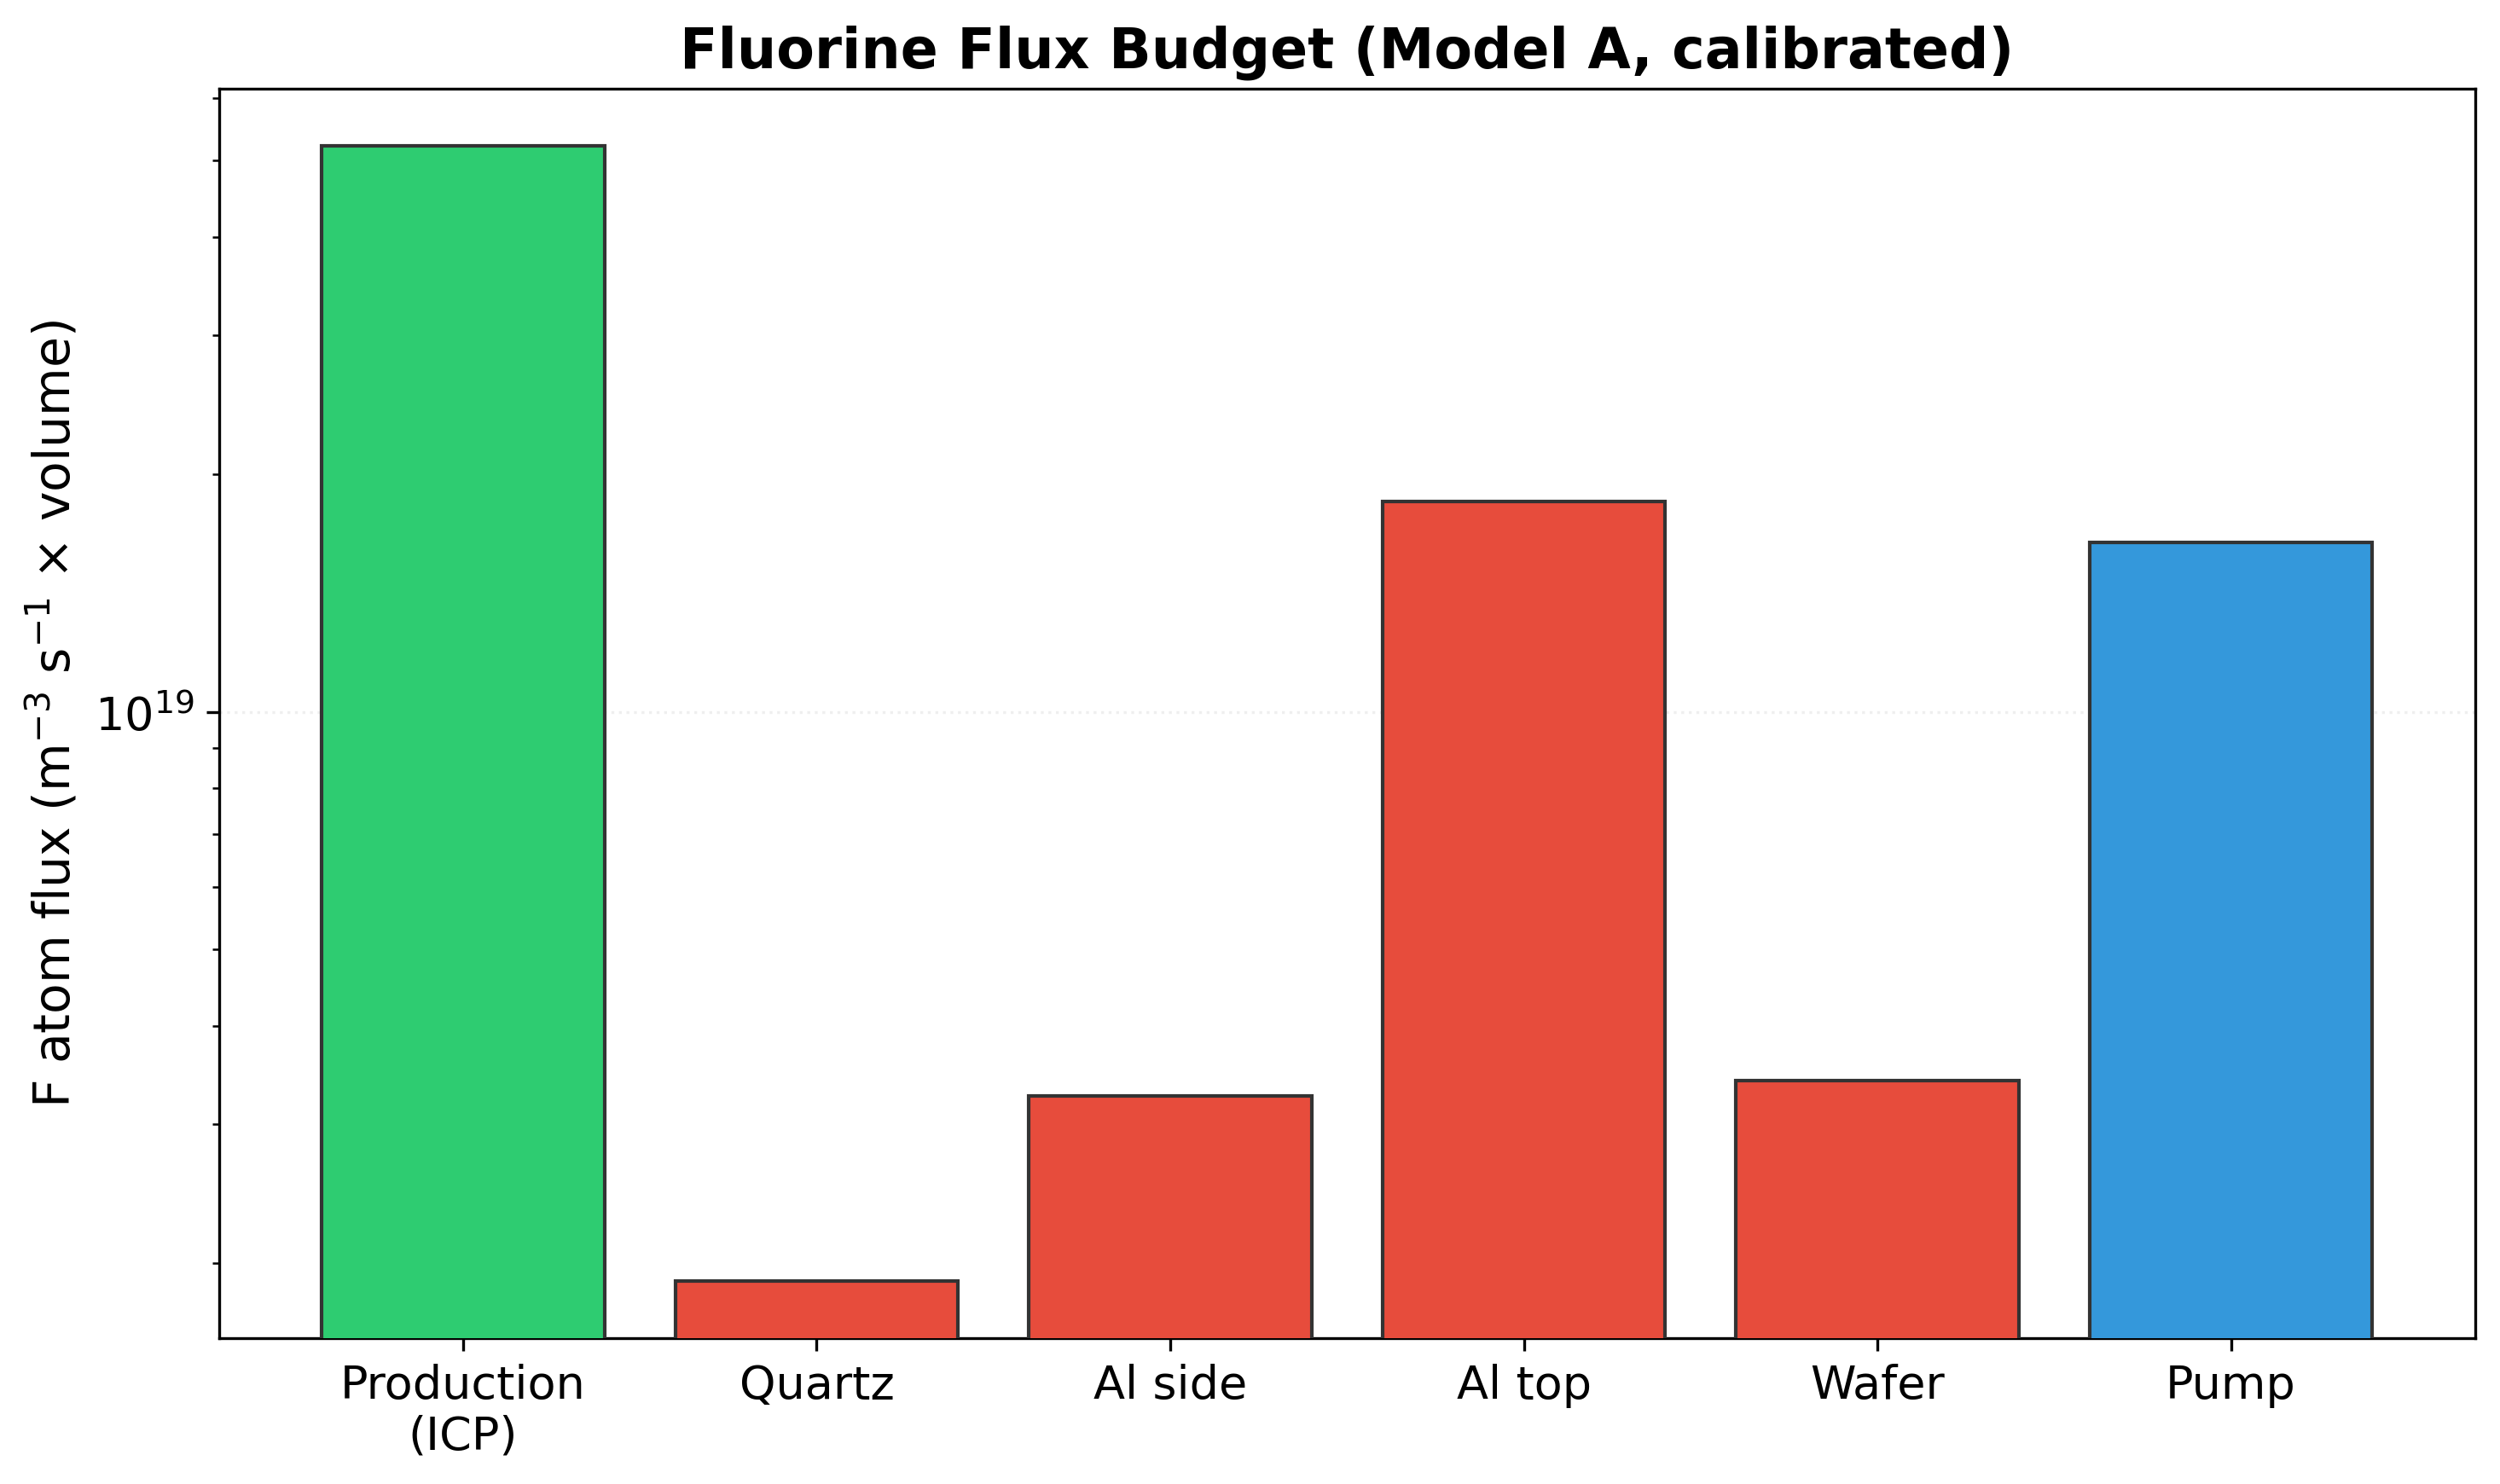
\includegraphics[width=\linewidth]{flux_budget.png}\\
\small Species flux budget at wafer surface
\column{0.48\textwidth}
\centering
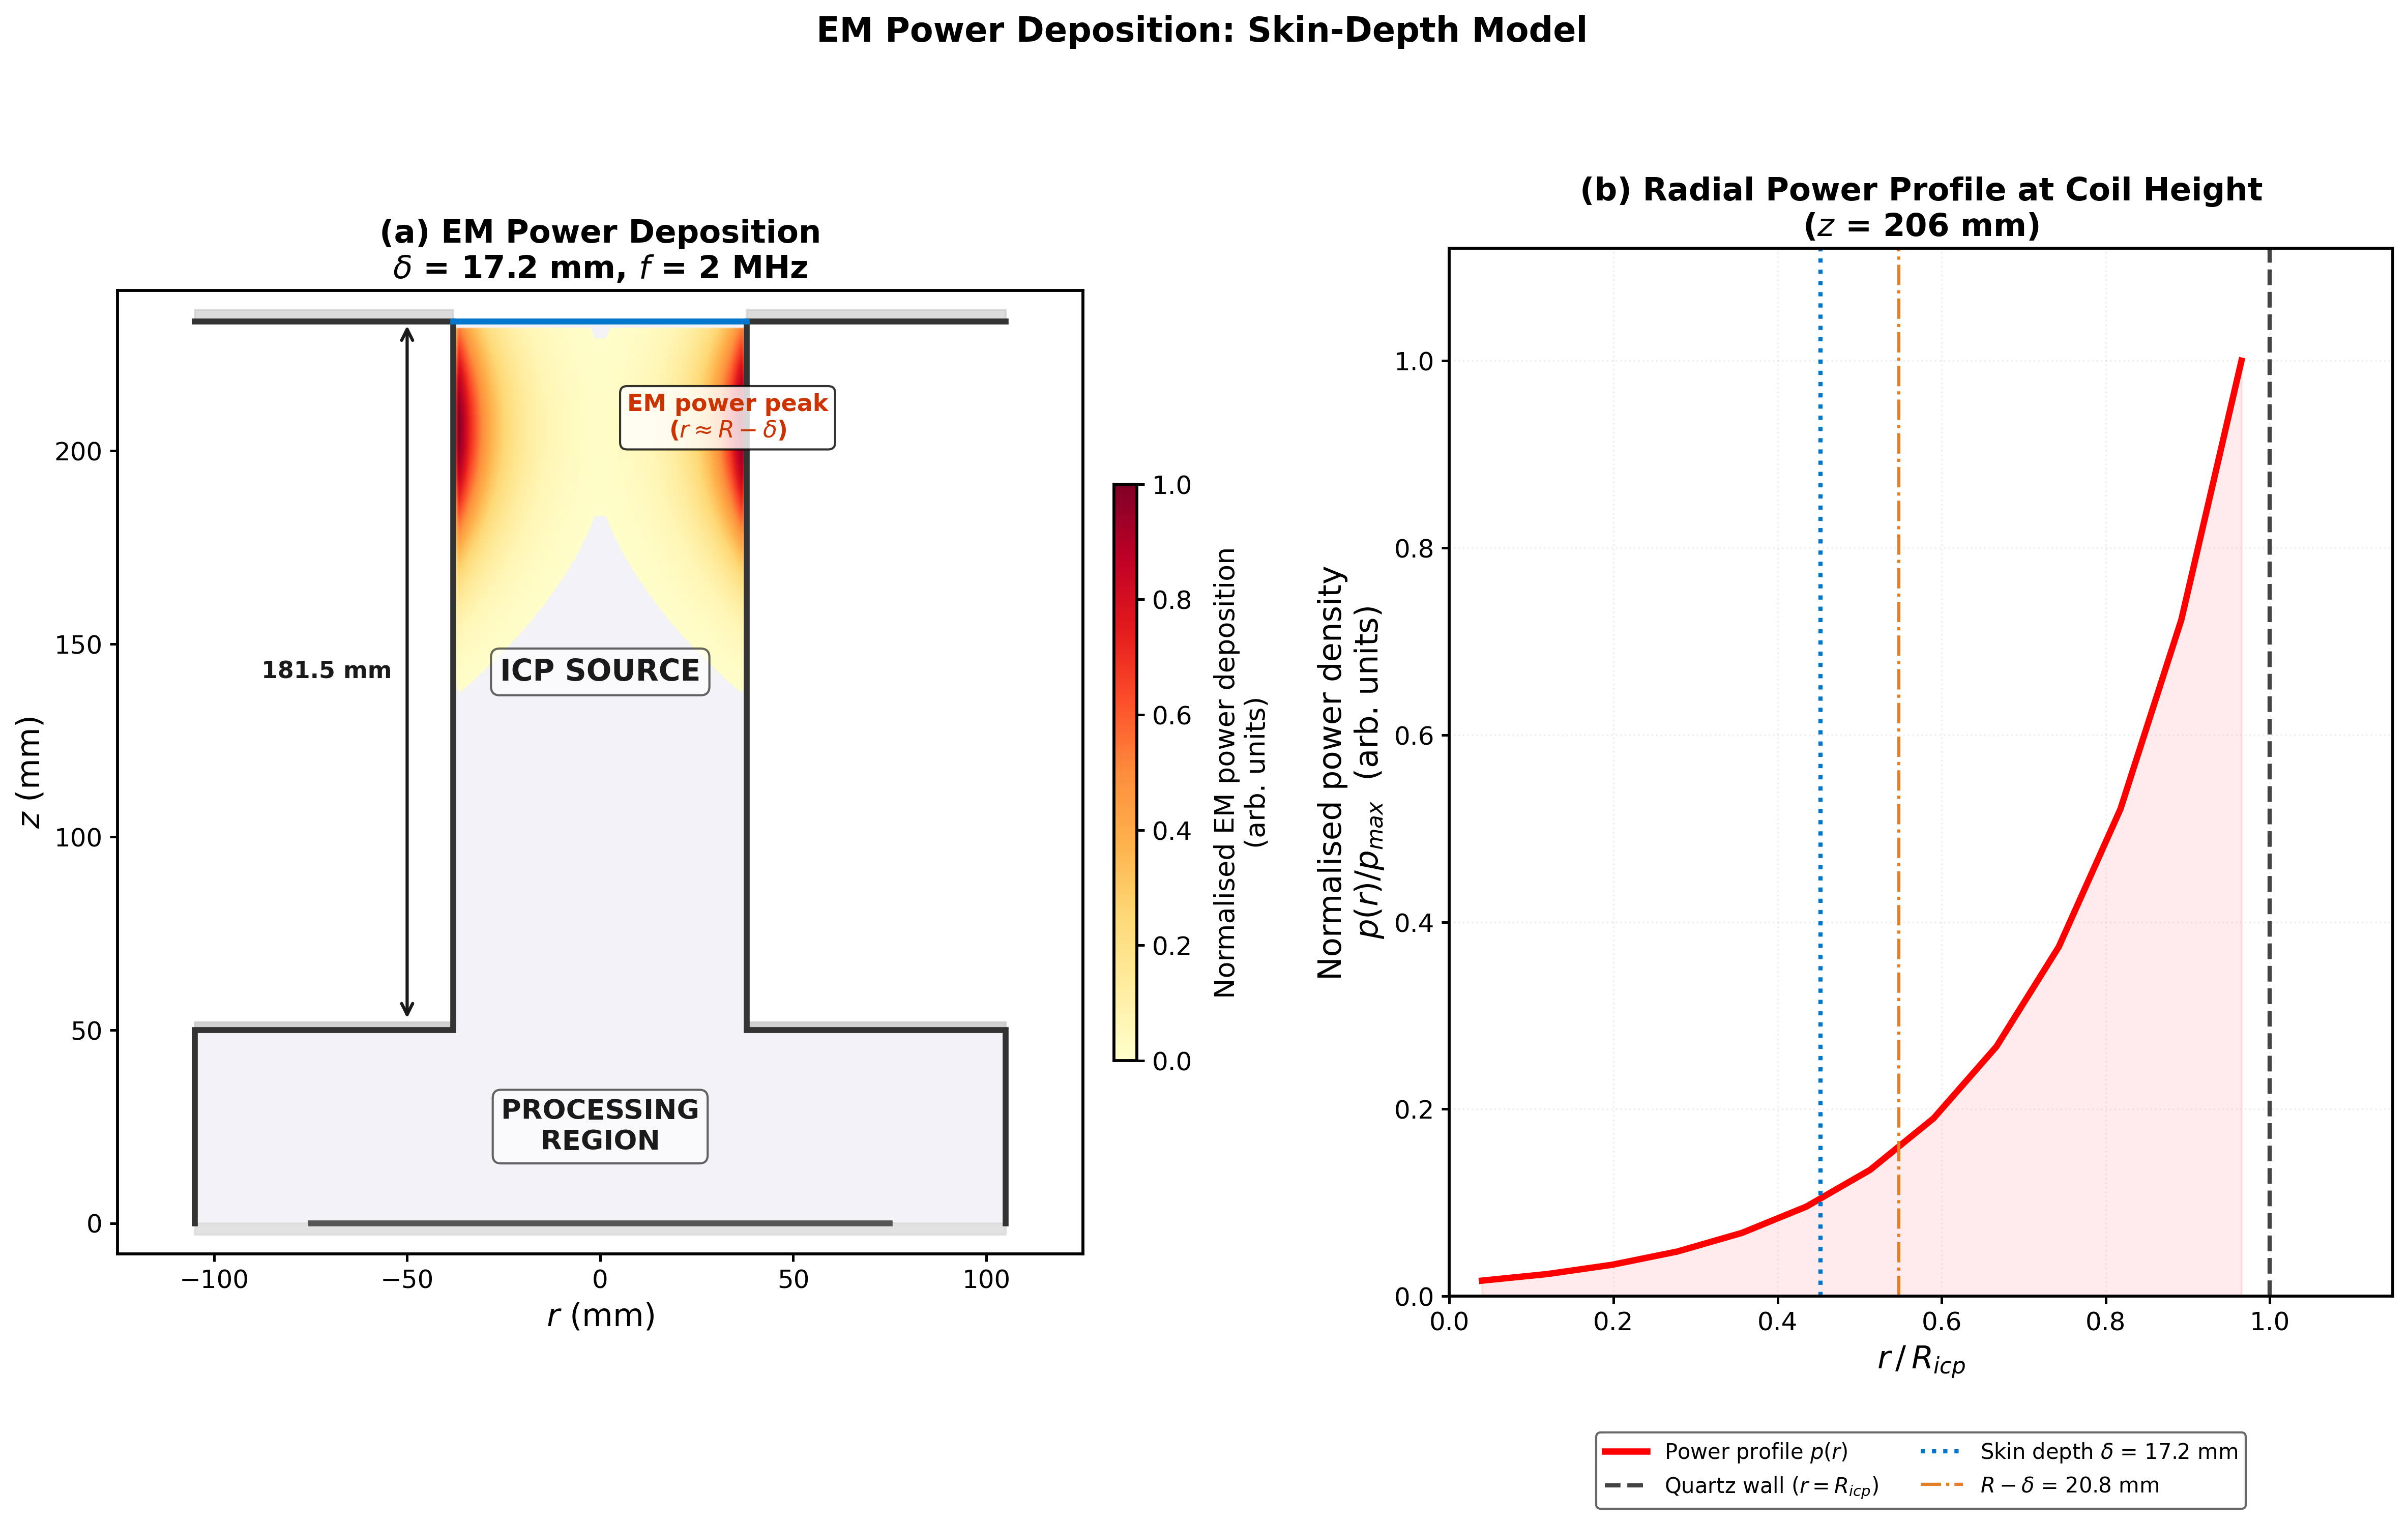
\includegraphics[width=\linewidth]{em_power_deposition.png}\\
\small Electromagnetic power deposition map
\end{columns}
\end{frame}

\end{document}
